\documentclass[9pt,mathserif,unknownkeysallowed,xcolor=dvipsnames]{beamer}
%\documentclass[9pt,mathserif,handout]{beamer}



\usetheme{default}
%\usecolortheme{seagull}
%\usecolortheme{rose}
%\usecolortheme{beaver}
%\usecolortheme{orchid}
%\usecolortheme{sidebartab}
\usefonttheme[onlylarge]{structurebold}
\setbeamerfont*{frametitle}{size=\normalsize,series=\bfseries}
\setbeamertemplate{navigation symbols}{}%remove navigation symbols 
%\setbeamertemplate{section in head/foot shaded}[default][30]
%\setbeamertemplate{subsection in head/foot shaded}[default][20]  
\setbeamertemplate{headline}[text line]%
{\parbox{1.063\textwidth}{\ \hfill \raisebox{-1.2\height}[0pt][0pt]{{
\includegraphics[width=2.2cm]{Images/FULogo-RGB}}}}}
% {\parbox{1.063\textwidth}{\flushright 
% \raisebox{-1.2\height}{
\includegraphics[width=2.5cm]{/Users/christophbenzmuellerimac/chris/trunk/tex/sty/FU/FULogo-RGB}}\\  
% \raisebox{-1.2\height}[0pt][0pt]{\includegraphics[width=.7cm]{logoPotsdam}}}}
\setbeamertemplate{footline}
{
\begin{beamercolorbox}[wd=\textwidth,ht=3ex,dp=1.5ex,center,leftskip=2em,rightskip=2em]%
{title in head/foot} 
C. Benzm\"uller, 2015\,-----\,\insertshorttitle \hfill \insertframenumber
\end{beamercolorbox}
}
\setbeamercovered{transparent}


%\usepackage{etex}
\usepackage[english]{babel}
\usepackage[latin1]{inputenc}
\usepackage{times}
\usepackage[T1]{fontenc}
%\usepackage{verbatim}
\usepackage{colortbl}
%\usepackage{array}

%\usepackage{amsmath}
%\usepackage{amssymb}
\usepackage{amsfonts}
\usepackage{pxfonts}
\usepackage{amsthm}
\usepackage{graphicx}
\usepackage{stmaryrd}
%\usepackage{latexsym}
\usepackage[makeroom]{cancel}

\usepackage{bussproofs}
\usepackage{proof}

\usepackage{fancybox}
\usepackage{fancyvrb}

%\usepackage{pstricks,vscolors}
\usepackage{etex}

\usepackage{pgf,pgfarrows,pgfnodes}

%\usepackage[final]{movie15}
\usepackage{multimedia}

% \usepackage{tikz}
% \usepackage{pgfgantt}
% \usepackage{chronology}


%\usepackage{rotating}

% Sequent Calculus Proof Settings
\EnableBpAbbreviations
\def\fCenter{\mbox{\ $\vdash$\ }}

\usepackage{calculi}


\usepackage{tikz}
\usetikzlibrary{positioning}
\usetikzlibrary{arrows}
\usetikzlibrary{automata,positioning}

\newcommand{\imp}{\rightarrow}
\newcommand{\biimp}{\leftrightarrow}
\newcommand{\all}{\forall}
\newcommand{\allq}{\forall}
\newcommand{\ex}{\exists}
\newcommand{\exq}{\exists}
\newcommand{\seq}{\vdash}
\newcommand{\nec}{\Box} % necessarily
\newcommand{\pos}{\Diamond} % possibly
\newcommand{\ess}[2]{#1 \ \mathit{ess.} \ #2}
\newcommand{\NE}{\mathit{NE}}
\newcommand{\sep}{\;|\;}

\newcommand{\fns}{\!\rightarrow\!}
\newcommand{\hs}{\! :: \!}
\newcommand{\br}{\rightarrow_\beta}


\newcommand{\s}{\qquad}


  \newcommand{\chriscite}[1]{{\small \textcolor{gray}{[#1]}}}

\def\modal#1{\boldsymbol{#1}}
\def\mfalse{\modal\bot}
\def\mtrue{\modal\top}
\def\mnot{\modal\neg\,}
\def\mor{\,\modal\vee\,}
\def\mand{\,\modal\wedge\,}
\def\mimpl{\,\modal\supset\,}
\def\miff{\,\modal\Leftrightarrow\,}
\def\mball#1{\modal\Box_{#1}\,}
\def\mdexi#1{\modal\Diamond_{#1}\,}
\def\mall#1{\modal{\forall}{#1}\lambdot\,}
\def\mallprop#1{\modal{\forall^{p}}{#1}\lambdot\,}
\def\mallind#1{\modal{\forall^{\mu}}{#1}\lambdot\,}
\def\mexi#1{\modal{\exists}{#1}\lambdot\,}
\def\mpi{\modal{\Pi}\,}
\def\mvalid{\modal{\texttt{valid}}} 

\def\typearrow{\shortrightarrow}
\def\worldtype{\iota}
\def\indtype{\mu}


\def\lambdot{\rule{0.6mm}{0.6mm}\hspace{0.4ex}} 
%\def\all#1{\forall #1\lambdot}
%\def\exi#1{\exists #1\lambdot}
%\def\lam#1{\lambda #1\lambdot}


\newcommand\entity[1]{\text{\textrm{#1}}}
\def\QHL{\entity{QHL}}
\def\QML{\entity{HOML}}
\def\NOM{\entity{NOM}}
\def\SVAR{\entity{SVAR}}
\def\CON{\entity{CON}}
\def\FVAR{\entity{FVAR}}
%\def\IC{\entity{IC}}
\def\FSYM{\entity{FSYM}}
\def\RSYM{\entity{RSYM}}
\def\QHLSTT{\entity{QHLSTT}}
\def\QMLSTT{\entity{QMLSTT}}
\def\IV{\entity{IV}}
\def\PV{\entity{PV}}
\def\SYM{\entity{SYM}}
\def\IVSTT{\entity{IVSTT}}
\def\PVSTT{\entity{PVSTT}}
\def\SYMSTT{\entity{SYMSTT}}
\def\SSTT{\entity{SSTT}}
\def\AR{\entity{AR}}
\def\STT{\entity{STT}\xspace}

\def\QKPIm{\entity{QK}\pi^-\xspace}
\def\QKPI{\entity{QK}\pi\xspace}
\def\QKPIp{\entity{QK}\pi^+\xspace}
\def\QSFPIm{\entity{QS5}\pi^-\xspace}
\def\QSFPI{\entity{QS5}\pi\xspace}
\def\QSFPIp{\entity{QS5}\pi^+\xspace}

\def\stt{\entity{STT}\xspace}
\def\tt{\entity{STT}}
\def\lm{\entity{MM}\xspace}
\def\ipl{\entity{IPL}\xspace}
\def\HOML{\entity{HOML}\xspace}
\def\HOL{\entity{HOL}\xspace}

\def\worldtype{\mu}
\def\indtype{\iota}
\def\mutype{\mu}
\def\boola{\omicron}
\def\boolb{\hat{\omicron}}

\def\ar{\shortrightarrow}

\newcommand\hol[1]{\boldsymbol{#1}}
\newcommand\lift[1]{\lceil #1 \rceil}
\newcommand\llift[1]{\dot{#1}}

\usepackage{xparse}

\NewDocumentCommand{\framecolorbox}{oommm}
 {% #1 = width (optional)
  % #2 = inner alignment (optional)
  % #3 = frame color
  % #4 = background color
  % #5 = text
  \IfValueTF{#1}
   {%
    \IfValueTF{#2}
     {\fcolorbox{#3}{#4}{\makebox[#1][#2]{#5}}}
     {\fcolorbox{#3}{#4}{\makebox[#1]{#5}}}%
   }
   {\fcolorbox{#3}{#4}{#5}}%
 }

\newenvironment{transitionframe}[2]
{
\begin{frame}{} \Large
\centering
\colorbox{#2}{\includegraphics[height=.6\textheight]{#1}}
\vfill
}
{

\end{frame}
}

\newenvironment{changemargin}[2]{% 
  \begin{list}{}{% 
    \setlength{\topsep}{0pt}% 
    \setlength{\leftmargin}{#1}% 
    \setlength{\rightmargin}{#2}% 
    \setlength{\listparindent}{\parindent}% 
    \setlength{\itemindent}{\parindent}% 
    \setlength{\parsep}{\parskip}% 
  }% 
\item[]
}{\end{list}} 


\setlength{\fboxsep}{3pt}%
\setlength{\fboxrule}{2pt}%


\title{On a (Quite) Universal Theorem Proving Approach and its Application to Metaphycis}

\author{\vskip-2em \textbf{Christoph Benzm\"{u}ller}\thanks{
   Supported by DFG Heisenberg Fellowship  BE 2501/9-1/2}, FU Berlin
 \\[.5em]
{\small jww: \textbf{B. Woltzenlogel-Paleo}, L. Paulson , C. Brown,
  G. Sutcliffe 
  and  many others! \\[.5em]Tableaux 2015 \\[-1.2em]
}
}


%\institute{Dagstuhl Seminar 15381 - Information from Deduction: Models and Proofs} 
%\institute{jww Bruno Woltzenlogel-Paleo}

%\date[10.02.2015]{February 10, 2015}
\date{\today}

\begin{document}


% \begin{frame}{Towards Computational Metaphysics}{Techniques and Tools for
% Knowledge Representation and Reasoning in Expressive Ontologies \\ Christoph Benzm\"{u}ller, Freie Universität Berlin}
% \includemovie[autopause,autoplay,autoresume,poster=/Users/cbenzmueller/chris/trunk/tex/talks/2015-TV/Movie1.pdf]{9cm}{6cm}{/Users/cbenzmueller/chris/trunk/tex/talks/2015-TV/Movie1.mov}
% \end{frame}

\begin{frame}\centering
  \titlepage 
\vskip-1.5cm
\colorbox{black!50}{
\movie[height=5cm,width=8cm,loop]{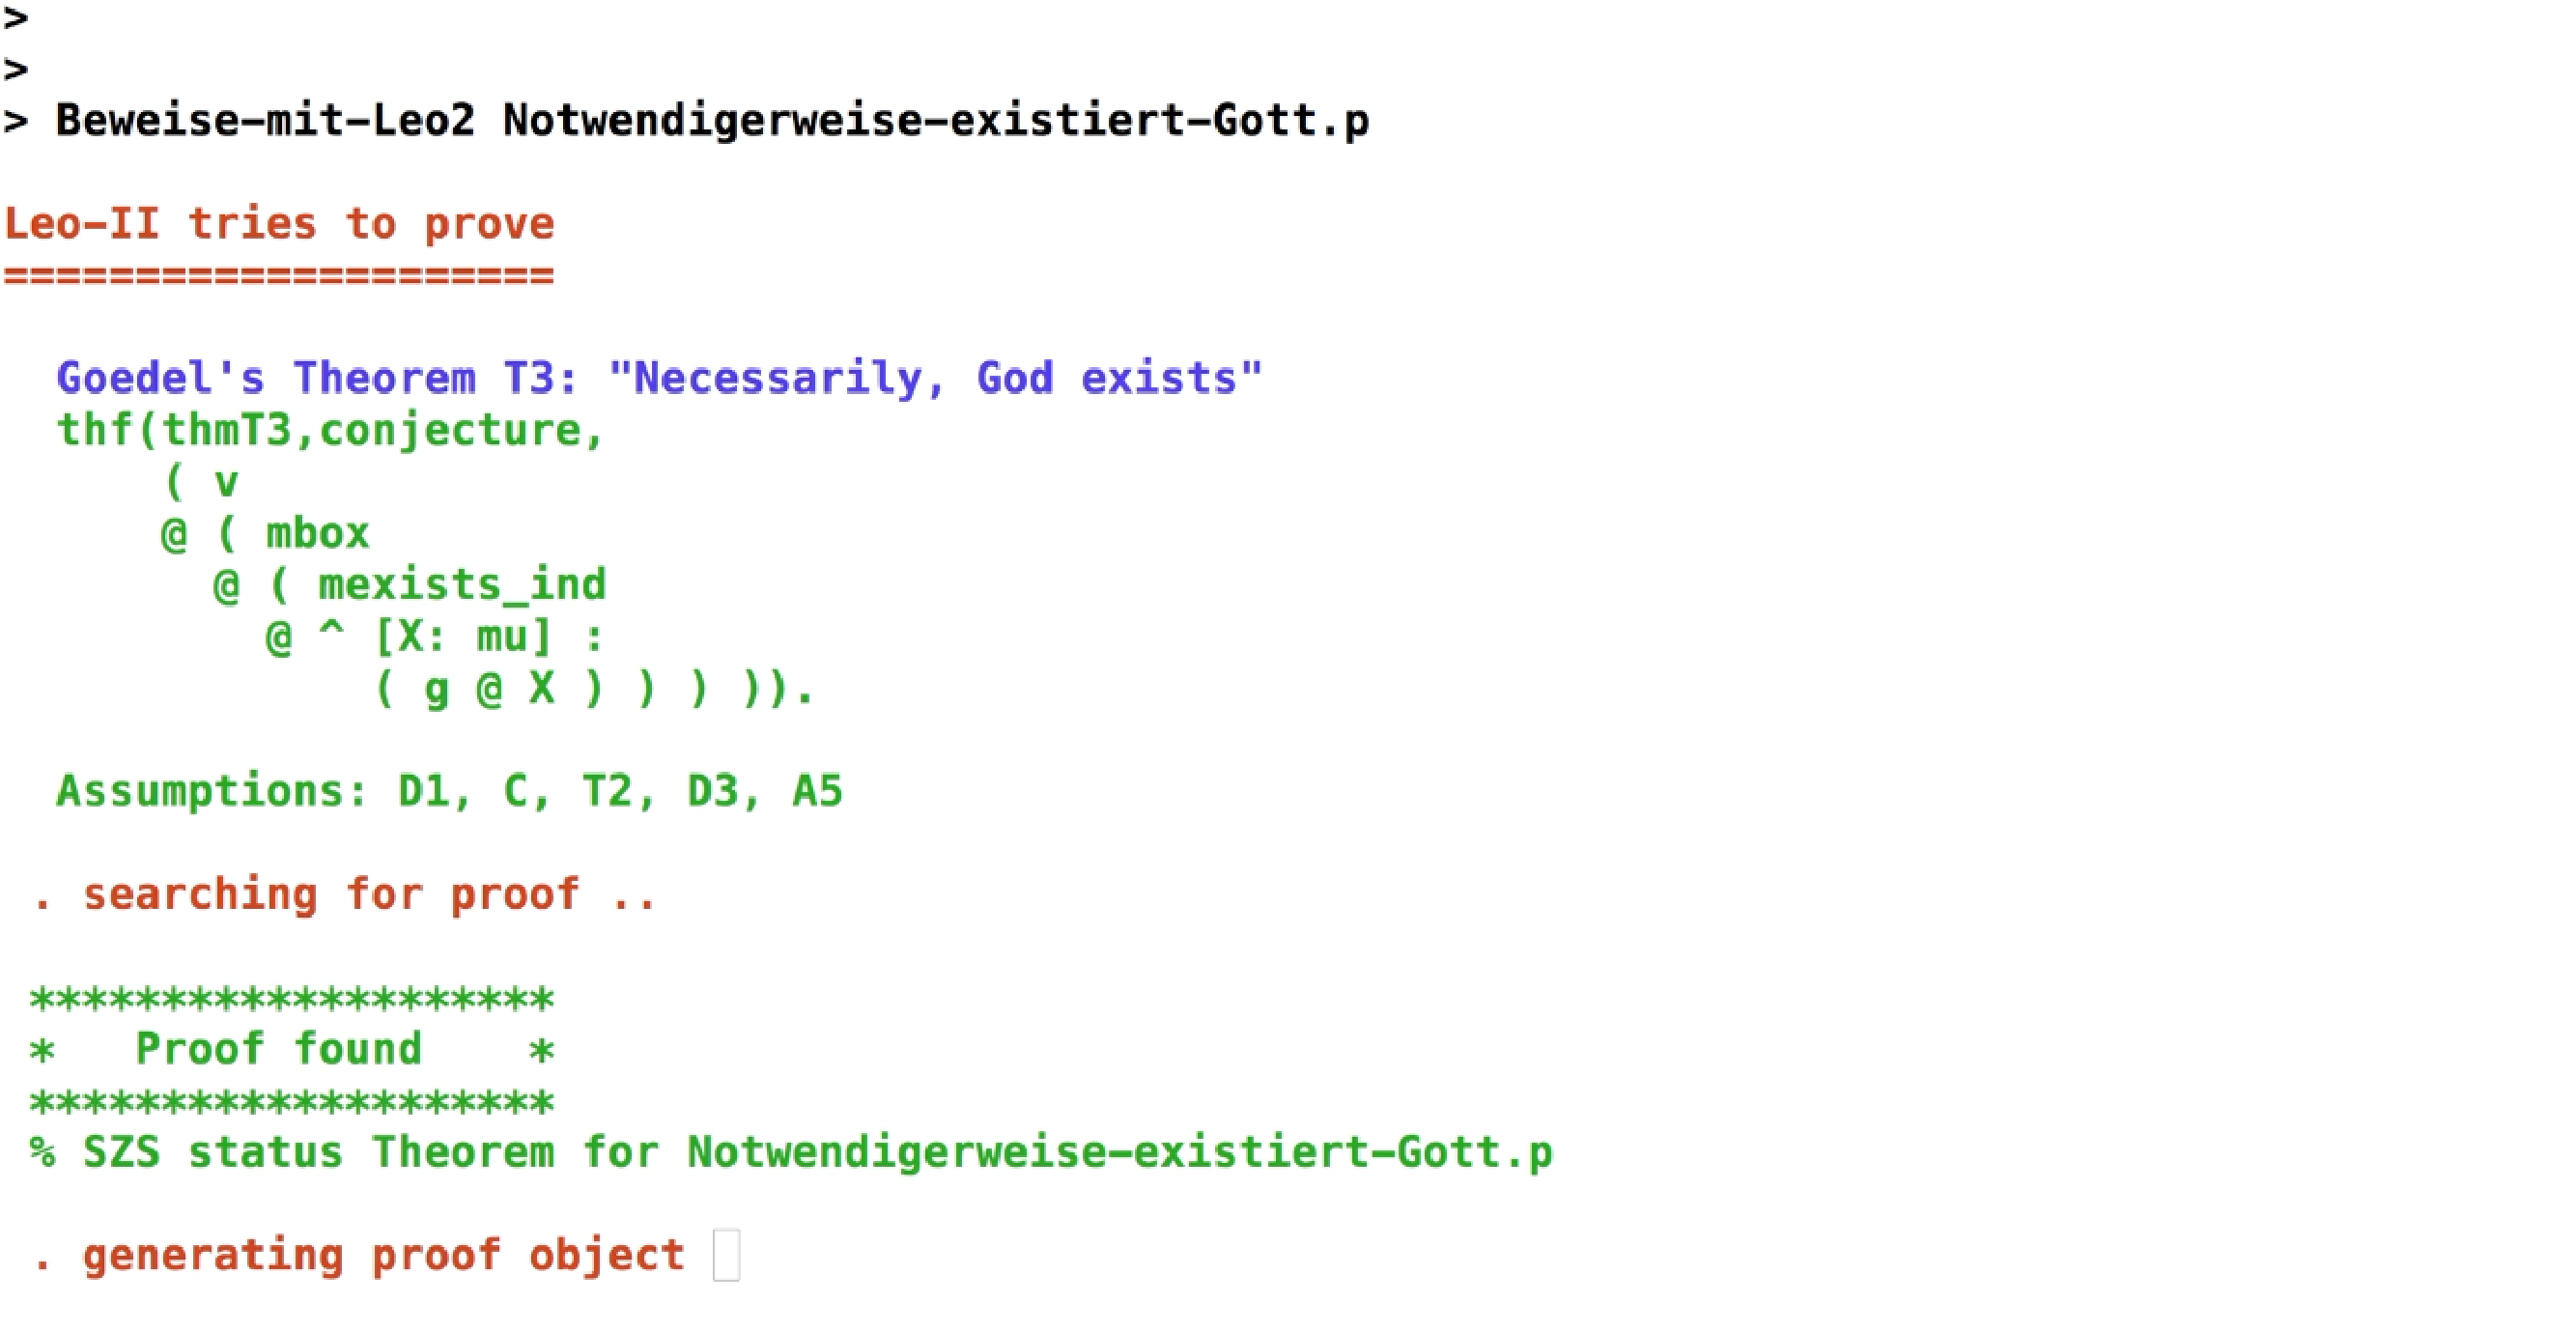
\includegraphics[height=5cm,width=8cm]{./Images/Movie1.pdf}}{./Images/Movie1.mov}
%\includemovie[autopause,autoplay,autoresume,poster=/Users/cbenzmueller/chris/trunk/tex/talks/2015-TV/Movie1.pdf]{8cm}{4cm}{/Users/cbenzmueller/chris/trunk/tex/talks/2015-TV/Movie1.mov}
}

%{\small \, \hfill jww Bruno Woltzenlogel-Paleo \hfill}
%\colorbox{gray}{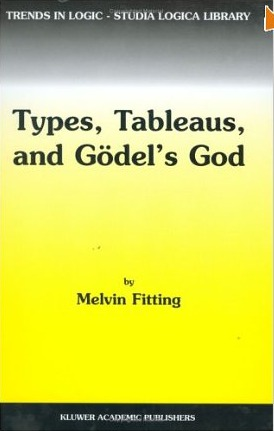
\includegraphics[height=2.5cm]{Images/Books/buch7.jpg} }
%\hfill
%\colorbox{gray}{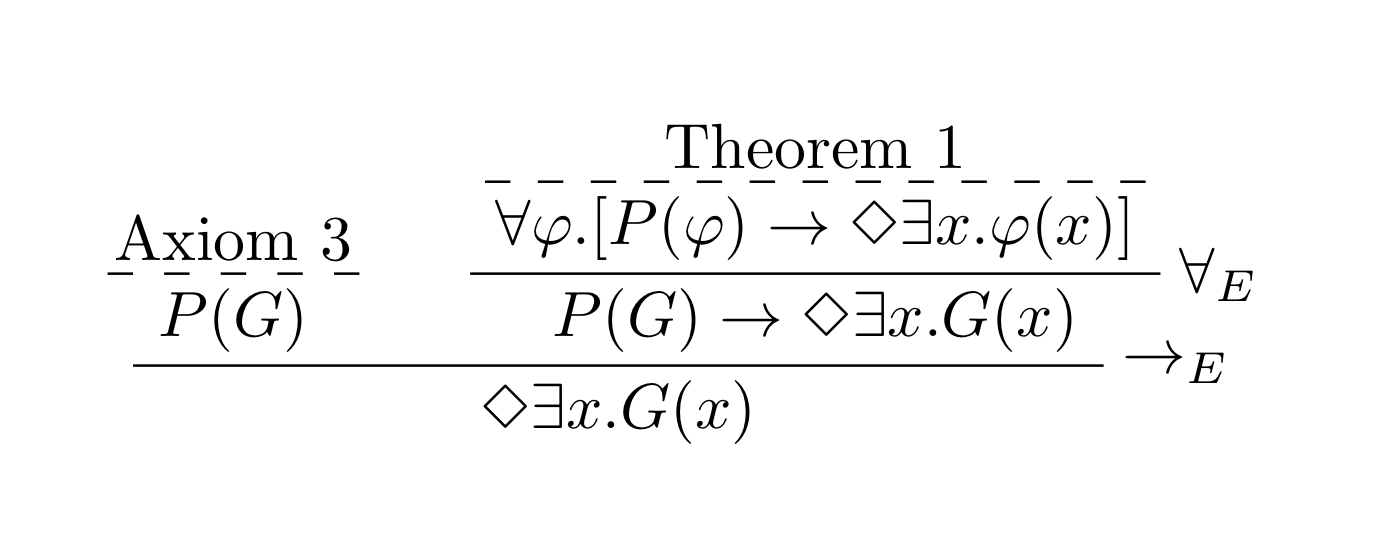
\includegraphics[height=2.5cm]{Images/ND.png}}
%\hfill \begin{footnotesize}A gift to \textbf{Priest Edvaldo} and his church in Piracicaba, Brazil\end{footnotesize}
\end{frame}




\begin{frame}{Talk Outline}
  % \begin{itemize}
  % \item 
    \textbf{A: HOL as a Universal (Meta-)Logic via Semantic Embeddings}
\vfill


%   % \item 
%     \textbf{Utilizing Countermodels from Nitpick in Meta-Logical Reasoning}
%     \begin{itemize}
%     \item Verification of the modal logic cube
%     \item Countermodels for false conjectures exploited for finding/formulating
%        appropriate lemmata
%     \item Schematic process can in principle be fully automated (no
%       brainer)
%     \item Applicable for the exploration of other metalogical relationships
%     \end{itemize}
% \vfill

  % \item
    \textbf{B: HOL ATPs contributed New Knowledge in Metaphysics}

\vfill
\begin{center}
{\colorbox{gray}{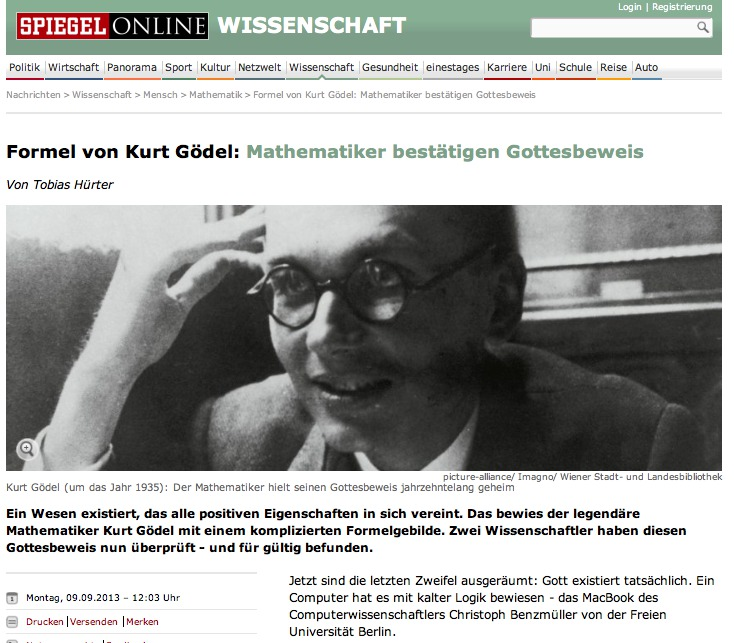
\includegraphics[width=.6\textwidth]{./Images/News/spiegel1}}}
\end{center}
 %    \begin{itemize}
%     \item Detection of inconsistency in G\"odel's variant of the ontological argument
%     \item LEO-II proof contains the intuitive proof idea --- but it is hard too grasp
%     \item Reconstruction of proof in Isabelle/HOL
%     \end{itemize}
% %  \end{itemize}
\end{frame}

\begin{frame}{} \small
\vskip1em
\begin{minipage}{.56\textwidth} 
\onslide*<0-1>{
\onslide*<0>{\colorbox{gray}{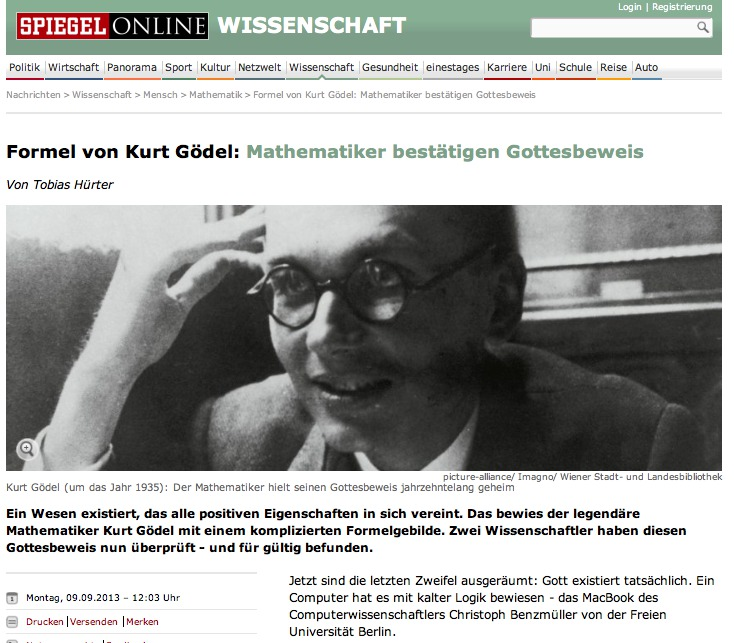
\includegraphics[width=\textwidth]{./Images/News/spiegel1}}}
\onslide*<1>{\colorbox{gray}{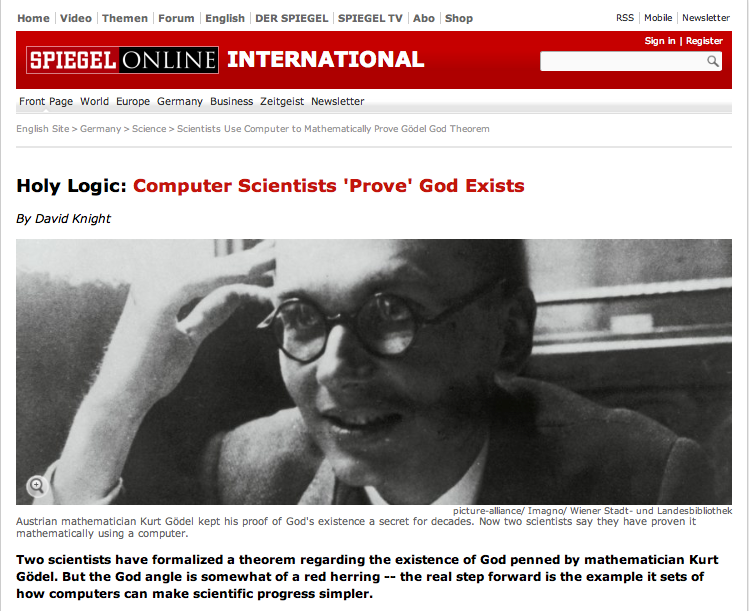
\includegraphics[width=\textwidth]{./Images/News/spiegel2}}}
\vskip1em
Germany \\
- Telepolis \& Heise \\
- Spiegel Online \\
- FAZ \\
- Die Welt \\
- Berliner Morgenpost \\
- Hamburger Abendpost \\
- \ldots \\
}
\onslide*<2>{\colorbox{gray}{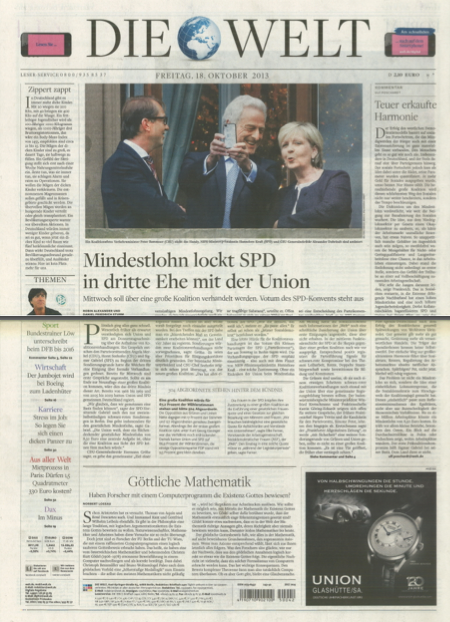
\includegraphics[width=\textwidth]{./Images/News/welt}}}
\end{minipage} \hfill
%
\begin{minipage}{.3\textwidth}
Austria \\
- Die Presse \\
- Wiener Zeitung \\
- ORF \\
- \ldots \\

Italy \\
- Repubblica \\
- Ilsussidario \\
- \ldots \\

% Russia \\
% - \ldots \\

India \\
- DNA India \\
- Delhi Daily News \\
- India Today \\
- \ldots \\

US \\
- ABC News \\
- \ldots \\

International \\
- Spiegel International \\
- Yahoo Finance \\
% - CNET \\
- United Press Intl. \\
- \ldots \\
\end{minipage}
\end{frame}

\begin{frame} \large
\colorbox{gray}{
\includegraphics[width=\textwidth]{./Images/News/MacBookGrab}} 
% \pause
% \vfill
% Are we in contact with Steve Jobs? \hfill No \\[2em]
% Do you really need a MacBook to obtain the results? \hfill No \\[2em]
% Did Apple send us some money? \hfill No \\
% \, \hfill (but maybe they should)
\vfill
%\pause
\normalsize
See more serious and funny news links at \\ 
\textbf{\url{https://github.com/FormalTheology/GoedelGod/tree/master/Press}}
\end{frame}



\begin{transitionframe}{./Images/open-brain}{black}%$
  \centering
 \textbf{Part A: \\ HOL as a Universal (Meta-)Logic via Semantic Embeddings}
 %\\ into Higher-Order Logic}
 %\textbf{Embedding Higher-Order Modal Logic \\ into Higher-Order
 %Logic}
\end{transitionframe}


\begin{frame}{HOL as a Universal (Meta-)Logic via Semantic Embeddings}
\scalebox{1.7}{
\begin{tikzpicture}[->,>=stealth',shorten >=1pt,auto,node distance=2cm,
                    semithick]
  \tikzstyle{every state}=[fill=none,draw=none,text=black]

  \node[state]         (Z1)                      {};
  \node[state]         (Z2) [right of=Z1] {\textcolor{Blue}{HOL}};
  \node[state]         (Z3) [right of=Z2] {};
 \node[state]         (A1)     [below of=Z1]
 {\begin{minipage}{1.5cm}{\begin{center} Logic \textcolor{red}{L} \\ Syntax \end{center}}\end{minipage}};
 \node[state]         (A2)     [below of=Z2] {};
 \node[state]         (A3)     [below of=Z3]
 {\begin{minipage}{1.5cm}{\begin{center}  Logic \textcolor{red}{L} \\ Semantics  \end{center}}\end{minipage}};

 

  \path
        (Z2) edge             node {} (A1)
        (Z2) edge             node {} (A2)
        (Z2) edge             node {} (A3)
        (A1) edge             node {} (A3)
        (A3) edge             node {} (A1);
\end{tikzpicture}
}

\pause

\textbf{Examples for \textcolor{red}{L} we have already studied}:

\textcolor{red}{\small Modal Logics, Conditional Logics, Intuitionistic Logics, Access
Control Logics, Nominal Logics, Multivalued Logics (SIXTEEN), Logics
based on Neighborhood Semantics, (Mathematical) Fuzzy Logics,
Paraconsistent Logics, \ldots}

\vskip.5em
\textbf{Works also for (first-order \& higher-order) quantifiers}
\end{frame}

\begin{frame}{Embedding Approach --- Idea}
\textcolor{Blue}{HOL (meta-logic)}\hfill \textcolor{Blue}{$\varphi$}
::= \textcolor{Blue!60}{\rule{6cm}{3mm}}\\[.5em]

\textcolor{red}{Your-logic (object-logic)}\hfill \textcolor{red!60}{$\psi$} ::=
  \textcolor{red!60}{\rule{6cm}{3mm}}\\[1em]

Embedding of \textcolor{red!60}{\rule{.5cm}{3mm}} in\ \textcolor{Blue!60}{\rule{.5cm}{3mm}}
\begin{align*}
\textcolor{red!60}{\rule{1cm}{3mm}} & = \textcolor{Blue!60}{\rule{5cm}{3mm}}\\
\textcolor{red!60}{\rule{1cm}{3mm}} & = \textcolor{Blue!60}{\rule{5cm}{3mm}}\\
\textcolor{red!60}{\rule{1cm}{3mm}} & = \textcolor{Blue!60}{\rule{5cm}{3mm}}\\
\textcolor{red!60}{\rule{1cm}{3mm}} & = \textcolor{Blue!60}{\rule{5cm}{3mm}}
\end{align*}

Embedding of meta-logical notions on
\textcolor{red!60}{\rule{.5cm}{3mm}} in\
\textcolor{Blue!60}{\rule{.5cm}{3mm}}
\begin{align*}
\textcolor{brown}{valid} & = \textcolor{Blue!60}{\rule{5cm}{3mm}}\\
\textcolor{brown}{satisfiable} & = \textcolor{Blue!60}{\rule{5cm}{3mm}}\\
\textcolor{red}{...} & = \textcolor{Blue!60}{\rule{5cm}{3mm}}
\end{align*}

Pass this set of equations to a higher-order automated theorem prover
\end{frame}



\begin{frame}{Embedding Approach --- HOML in HOL}\large
\begin{changemargin}{-.5cm}{0cm}

\textcolor{Blue}{HOL}\hfill 
$\begin{array}{lll}
\textcolor{Blue}{s,t} & ::= & \textcolor{Blue}{C_\alpha}  \mid
\textcolor{Blue}{x_\alpha \mid (\lambda{x_\alpha} s_\beta)_{\alpha\typearrow\beta}} \mid \textcolor{Blue}{(s_{\alpha\typearrow\beta}\, t_\alpha)_\beta}
\mid \textcolor{Blue}{\neg s_o} \mid \textcolor{Blue}{s_o \vee t_o} \mid
\textcolor{Blue}{\forall {x_\alpha}\, t_o} 
\end{array}$ \\[.5em]
\textcolor{red}{HOML} \hfill
$\begin{array}{lll}\textcolor{red}{\varphi,\psi} & ::= &
  \textcolor{red}{\ldots}  \mid \textcolor{red}{\neg
    \varphi} \mid \textcolor{red}{\varphi \wedge \psi} \mid
  \textcolor{red}{\varphi \imp \psi}  \mid \textcolor{red}{\Box
    \varphi} \mid \textcolor{red}{\Diamond \varphi}  \mid
 \textcolor{red}{\forall {x_\gamma}\, \varphi} \mid
  \textcolor{red}{\exists {x_\gamma}\, \varphi} 
%\mid \textcolor{red}{\forall {P}\, \varphi} 
\end{array}$ \\[1em]

%\pause

\textcolor{red}{HOML} in \textcolor{Blue}{HOL}: \quad \textcolor{red}{HOML}
formulas $\textcolor{red}{\varphi}$ are mapped to
\textcolor{Blue}{HOL} predicates
$\textcolor{red}{\varphi_{\worldtype\typearrow o}}$\\
\qquad \qquad \qquad \qquad (explicit representation of labelled
formulas) \\[1em]

\pause

\begin{center}
\fcolorbox{Blue}{white}{
$\begin{array}{lcl} 
    \textcolor{red}{\mnot} & = & \textcolor{Blue}{
      \lambda{\varphi_{\worldtype\typearrow o}}\lambda{w_\worldtype}\neg \varphi w} \\ 
    \textcolor{red}{\mand} & = & \textcolor{Blue}{ 
      \lambda{\varphi_{\worldtype\typearrow o}}
      \lambda{\psi_{\worldtype\typearrow o}} \lambda{w_\worldtype}
      (\varphi w \wedge \psi w)} \\ 
    \textcolor{red}{\imp} & = & \textcolor{Blue}{ 
      \lambda{\varphi_{\worldtype\typearrow o}}
      \lambda{\psi_{\worldtype\typearrow o}} \lambda{w_\worldtype}
      (\neg \varphi w \vee \psi w)} \\[.5em] 
    \textcolor{red}{\forall} & = & \textcolor{Blue}{ 
      \lambda{h_{\gamma\typearrow(\worldtype \typearrow o)}}
      \lambda{w_\worldtype} \forall {d_\gamma} \, h d w} \\
    \textcolor{red}{\exists} & = & \textcolor{Blue}{ 
      \lambda{h_{\gamma\typearrow(\worldtype \typearrow o)}}
      \lambda{w_\worldtype} \exists {d_\gamma} \, h d w} \\[.5em]
    \alt<0>{\textcolor{Blue}{ 
      \forall {\varphi_{\worldtype\typearrow o}} \forall
      {w_\worldtype} [\ \ (\textcolor{red}{\Box} \varphi) w}& \equiv & \textcolor{Blue}{ 
      \forall {u_\worldtype}\, (\neg r w u \vee
      \varphi u)\ \ ]}}{\textcolor{red}{\Box} & = & \textcolor{Blue}{ 
      \lambda{\varphi_{\worldtype\typearrow o}} \lambda{w_\worldtype}
      \forall {u_\worldtype}\, (\neg r w u \vee
      \varphi u)}} \\ 
    \textcolor{red}{\Diamond} & = & \textcolor{Blue}{ 
      \lambda{\varphi_{\worldtype\typearrow o}} \lambda{w_\worldtype}
      \exists {u_\worldtype}\, (r w u \wedge
      \varphi u)} \\[.5em] 
    \text{\textcolor{brown}{valid}} & = & \textcolor{Blue}{
        \lambda{\varphi_{\worldtype\typearrow o}} \all{w_\worldtype}
        \varphi w}
\end{array}$
}  \quad \textcolor{Blue}{Ax} \alt<0>{}{{\footnotesize (polymorphic over $\gamma$)}}
\vskip1em
\end{center}

%\pause

\quad The equations in \textcolor{Blue}{Ax} are given as axioms to the \textcolor{Blue}{HOL} provers! \\

\end{changemargin}
\end{frame}


\begin{frame}{Embedding HOML in HOL} \large

\hskip-1em Example \\[.5em]

 \textcolor{red}{HOML} formula  \hfill \textcolor{red}{$\Diamond \exists x G(x)$}

\pause 

 \textcolor{red}{HOML} formula in \textcolor{Blue}{HOL}  \hfill
 $\text{\textcolor{brown}{valid}}\, \textcolor{red}{(\Diamond \exists
   x G(x))_{\worldtype\typearrow o}}$

\pause

expansion \hfill $\textcolor{Blue}{(\lambda \varphi \forall
  w_\worldtype \varphi\, w) \textcolor{red}{(\Diamond \exists x
    G(x))_{\worldtype\typearrow o}}}$ 

\pause

$\beta\eta$-normalisation \hfill $\textcolor{Blue}{\forall
  w_\worldtype (\textcolor{red}{(\Diamond \exists x
    G(x))_{\worldtype\typearrow o}}\, w)}$ 

\pause

expansion \hfill $\textcolor{Blue}{\forall
  w_\worldtype (\textcolor{red}{(\textcolor{Blue}{ 
      (\lambda{\varphi_{\worldtype\typearrow o}} \lambda{w_\worldtype}
      \exists {u_\worldtype}\, (r w u \wedge
      \varphi u))} \exists x
    G(x))_{\worldtype\typearrow o}}\, w)}$ 

\pause

$\beta\eta$-normalisation \hfill $\textcolor{Blue}{\forall
  w_\worldtype \exists {u_\worldtype} (r w u \wedge
      \textcolor{red}{(\exists x G(x))_{\worldtype\typearrow o}} u)}$ 

\pause

syntactic sugar \hfill $\textcolor{Blue}{\forall
  w_\worldtype \exists {u_\worldtype} (r w u \wedge
      \textcolor{red}{(\exists (\lambda x G(x)))_{\worldtype\typearrow
          o}} u)}$ 

\pause

expansion \hfill $\textcolor{Blue}{\forall
  w_\worldtype \exists {u_\worldtype} (r w u \wedge
      \textcolor{red}{(\textcolor{Blue}{( 
      \lambda{h_{\gamma\typearrow(\worldtype \typearrow o)}}
      \lambda{w_\worldtype} \exists {d_\gamma} \, h d w)} (\lambda x G(x)))_{\worldtype\typearrow o}} u)}$ 

% expansion, $\beta\eta$-normalisation \hfill $\textcolor{Blue}{\forall
%   w_\worldtype \exists {u_\worldtype} (r w u \wedge
%       \exists x \textcolor{red}{G(x)_{\worldtype\typearrow o}} u)}$ 

\pause

$\beta\eta$-normalisation \hfill $\textcolor{Blue}{\forall
  w_\worldtype \exists {u_\worldtype} (r w u \wedge
      \exists x G x u)}$ \\[1em]

\pause
\hskip-1em Expansion: \hfill user or prover may flexibly choose
expansion depth 

\pause
\vfill
\begin{block}{What are we doing?}
\vskip.5em
In order to prove that $\textcolor{red}{\varphi}$ is valid in \textcolor{red}{HOML}, \\
--> we instead prove that 
$\text{\textcolor{brown}{valid}}\,
\textcolor{red}{\varphi_{\worldtype\typearrow o}}$ can be derived
from \textcolor{Blue}{Ax} in \textcolor{Blue}{HOL}. \\[1em]

This can be done with interactive or automated \textcolor{Blue}{HOL} theorem provers.
\end{block}
%\pause
%\vfill
% \pause
% \hskip-1em For the experts: \hfill soundness and completeness wrt Henkin semantics
\end{frame}

\begin{frame}{Advantages of the Embedding Approach}
% \ \hfill \chriscite{Benzm\"ullerWoltzenlogelP., RW'2015, CSR'2015,
%   ECAI'2014, WADT'2014, AFP'2013} \\
% \ \hfill \chriscite{Benzm\"ullerPaulson, Logica Universalis, 2013} \\
% \ \hfill \chriscite{Benzm\"uller, IJCAI'2013} \\[2em]

\begin{enumerate}
\item \textcolor{red}{Pragmatics and convenience}:
  \begin{itemize}
  \item  implementing new provers made simple (even for not yet
    automated logics)
  \end{itemize}
\item \textcolor{red}{Availability}:
\begin{itemize}
  \item  simply  reuse and adapt our existing encodings (THF, Isabelle/HOL, Coq)
  \end{itemize}
\item \textcolor{red}{Flexibility}:
\begin{itemize}
  \item  rapid experimentation with logic variations and logic combinations 
  \end{itemize}
\item \textcolor{red}{Relation to labelled deductive systems}:
\begin{itemize}
  \item   extra-logical labels vs. intra-logical labels (here)
  \end{itemize} 
\item \textcolor{red}{Relation to standard translation}:
\begin{itemize}
  \item   extra-logical  translation vs. extended intra-logical translation (here)
  \end{itemize}
\item \textcolor{red}{Meta-logical reasoning}: 
\begin{itemize}
  \item  various examples already exist, e.g. verification of modal
  logic cube
  \end{itemize}
\item \textcolor{red}{Direct calculi and user intuition}: 
  \begin{itemize}
  \item  possible: tactics on top of embedding, hiding of embedding
  \end{itemize}
\item \textcolor{red}{Soundness and completeness}: 
  \begin{itemize}
  \item  already proven for many non-classical logics (wrt Henkin semantics)
  \end{itemize} 
\item \textcolor{red}{Cut-elimination}:
  \begin{itemize}
  \item  generic indirect result,  since HOL enjoys cut-elimination (Henkin semantics)
  \end{itemize}
\end{enumerate}
\end{frame}


\begin{frame}[t]{Advantage: \textcolor{red}{1. Pragmatics and
      convenience}}{implementing new provers made simple (even for not yet
    automated logics)}

\onslide*<1>{
\begin{block}{A very ``Lean'' Prover for HOML KB}
%\vskip1em
\scalebox{0.9}{
\colorbox{yellow!20}{
\begin{minipage}{\linewidth}
               \VerbatimInput[frame=single,%
               commandchars=\\\{\},%
               fontfamily=courier,fontseries=b,%
               fontsize=\tiny,%
               rulecolor=\color{green},%
               fillcolor=\color{yellow},%
               formatcom=\color{Blue},%
               framerule=0pt,%
               framesep=0pt,numbers=left]%
               {./DemoMaterial/DEMO-THF/Quantified_KB.ax}
%               {Axioms_annotated.ax}
\end{minipage}

}}

% Reading on Embedding: \hfill \chriscite{Benzm\"ullerPaulson, Logica
%   Universalis, 2013}
\vskip.5em
TPTP THF0 syntax: \hfill \chriscite{SutcliffeBenzm\"uller,   J.Formalized Reasoning, 2010}
\end{block}
}

\onslide*<2>{
\begin{block}{Approach is competitive}
\begin{itemize}
\item First-order modal logic: see experiments in \\ 
\ \hfill \chriscite{Benzm\"ullerOttenRaths, ECAI, 2012} \\
\ \hfill \chriscite{Benzm\"ullerRaths, LPAR, 2013} \\
\ \hfill \chriscite{Benzm\"uller, ARQNL, 2014}  \\
\item Higher-order modal logics:
\begin{center}
\textcolor{red}{There are no other systems yet!}
\end{center}
\end{itemize}
\end{block}
}
\end{frame}

\begin{frame}{Advantage: \textcolor{red}{2. Availability}}
{simply reuse and adapt our existing encodings (THF, Isabelle/HOL,
  Coq)}
\onslide*<1>{
\begin{block}{HOML in Isabelle/HOL}
\vskip1em
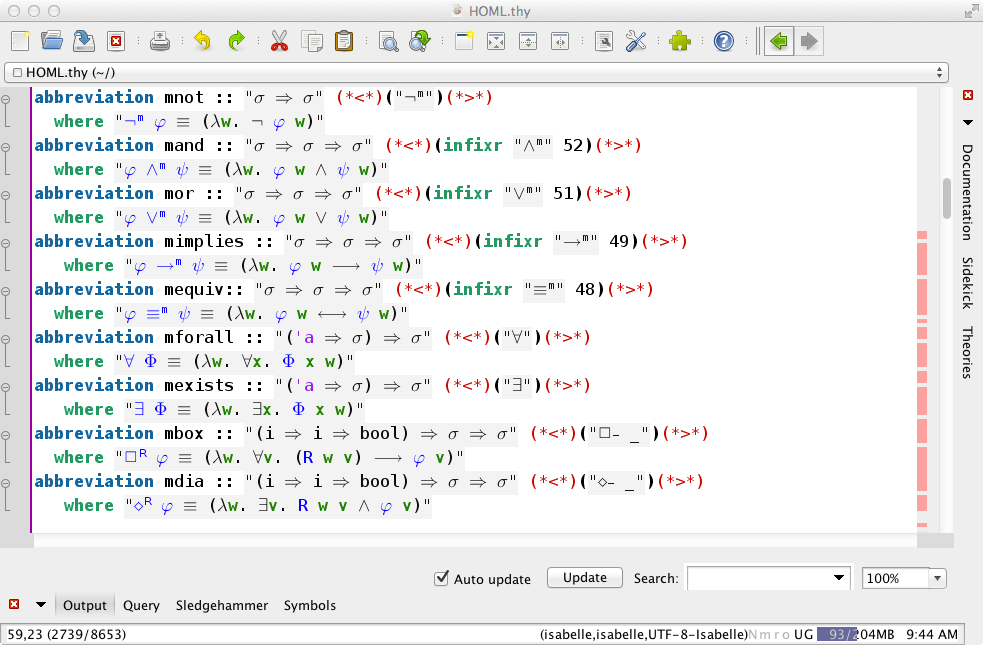
\includegraphics[height=7cm,width=10.5cm]{./Images/Isabelle-HOML}
\end{block}
}
\end{frame}


\begin{frame}[t]{Advantage: \textcolor{red}{3. Flexibility}}
{rapid experimentation with logic variations and logic combinations}

\large
\onslide*<2>{
\begin{block}{Possibilist vs. Actualist Quantification }
%\textbf{Modified Quantifiers:}
\vskip1em
$\textcolor{red}{\forall^{\phantom{va}}}  = \textcolor{Blue}{ 
      \lambda{h_{\gamma\typearrow(\worldtype \typearrow o)}}
      \lambda{w_\worldtype} \forall {d_\gamma} \, h d w}$ \hfill
    (constant domains)\\
\quad becomes \\
$\textcolor{red}{\forall^{va}}  = \textcolor{Blue}{ 
      \lambda{h_{\gamma\typearrow(\worldtype \typearrow o)}}
      \lambda{w_\worldtype} \forall {d_\gamma} \, (\textbf{ExInW}\, d w \imp
      h d w)}$ \hfill (varying domains)
\vskip1em
where \textbf{\textcolor{Blue}{ExInW}} is an existence predicate \\
\textcolor{gray}{\small (additional axioms: non-empty domains, denotation of constants \& functions)}
% \vskip1em
% \begin{itemize}
% \item domains are non-empty \hfill \textcolor{Blue}{$\forall{w_\worldtype}\exists{x_\mu}
% \textbf{exInW} x w$}\\[1em]

% \item denotation (constants \& functions) \hfill \textcolor{Blue}{$\forall{w_\worldtype}\textbf{exInW} c w$} \\
% \, \hfill  \textcolor{Blue}{$\forall{w_\worldtype} (\textbf{exInW} {t^1} w
% \wedge \ldots \wedge  \textbf{exInW} {t^n} w \supset
% \textbf{exInW}{(f\,t^1\ldots t^n)} w)$} \\[2em]
% \end{itemize}

% \textbf{Cumulative domains:}  \hfill
% \textcolor{Blue}{$\forall{x}\forall{v}\forall{w}  (\textbf{exInW} x
% v \wedge r v w \supset \textbf{exInW} x w)$}
\end{block}
}


\onslide*<1>{
\begin{block}{Postulating modal axioms or semantical constraints}
%\small
\hskip3em
\scalebox{1.5}{
\begin{tikzpicture}[->,>=stealth',shorten >=1pt,auto,node distance=2cm,
                    semithick]
  \tikzstyle{every state}=[fill=none,draw=none,text=black]

  \node[state]         (Z1)                      {};
  \node[state]         (Z2) [right of=Z1] {\textcolor{Blue}{HOL}};
  \node[state]         (Z3) [right of=Z2] {};
 \node[state]         (A1)     [below of=Z1] {};
 \node[state]         (A2)     [below of=Z2] {};
 \node[state]         (A3)     [below of=Z3] {};
  \path
        (Z2) edge             node {} (A1)
        (Z2) edge             node {} (A2)
        (Z2) edge             node {} (A3);
\end{tikzpicture}
}

\vskip-3em
\normalsize
\textbf{Sahlqvist axioms} \hfill \textbf{Semantical constraints}\\[.1cm]

\begin{tabular}{lllll}

M: &  $\textcolor{red}{\text{\textcolor{brown}{valid}}\ \forall
  \varphi (\Box^{\textcolor{black}{r}} \varphi \imp \varphi)}$ & $\leftrightarrow$
&
$\textcolor{Blue}{\forall x ({\textcolor{black}{r}} x x)}$ & (reflexivity) \\

B: & $\textcolor{red}{\text{\textcolor{brown}{valid}}\ \forall
  \varphi (\varphi \imp \Box^{\textcolor{black}{r}} \Diamond^{\textcolor{black}{r}} \varphi)}$ & $\leftrightarrow$
&
$\textcolor{Blue}{\forall x \forall y ({\textcolor{black}{r}} x y \imp {\textcolor{black}{r}} y x)}$  &
                                                              (symmetry) \\

D: & $\textcolor{red}{\text{\textcolor{brown}{valid}}\ \forall
  \varphi (\Box^{\textcolor{black}{r}} \varphi \imp \Diamond^{\textcolor{black}{r}} \varphi)}$ & $\leftrightarrow$
& 
$\textcolor{Blue}{\forall{x} \exists{y} ({\textcolor{black}{r}} x y)}$ & (serial) \\

4: & $\textcolor{red}{\text{\textcolor{brown}{valid}}\ \forall
  \varphi (\Box^{\textcolor{black}{r}}\varphi \imp \Box^{\textcolor{black}{r}} \Box^{\textcolor{black}{r}} \varphi)}$ & $\leftrightarrow$
&
$\textcolor{Blue}{\forall x \forall y \forall z ({\textcolor{black}{r}} x y \wedge {\textcolor{black}{r}} y z
  \imp {\textcolor{black}{r}} x z)}$ & (transitivity) \\

5: & $\textcolor{red}{\text{\textcolor{brown}{valid}}\ \forall
  \varphi (\Diamond^{\textcolor{black}{r}}\varphi \imp \Box^{\textcolor{black}{r}} \Diamond^{\textcolor{black}{r}} \varphi)}$ & $\leftrightarrow$
&
$\textcolor{Blue}{\forall x \forall y \forall z ({\textcolor{black}{r}} x y \wedge {\textcolor{black}{r}} x z
  \imp {\textcolor{black}{r}} y   z)}$&  (euclidean) \\

\end{tabular}
\end{block}
}
\normalsize

% \textbf{Non-Sahlqvist}:

% L\"ob: \quad $\textcolor{red}{\text{\textcolor{brown}{valid}}\ \forall
%   \varphi (\Box^{\textcolor{black}{r}}(\Box^{\textcolor{black}{r}}
% \varphi \imp \varphi) \imp \Box^{\textcolor{black}{r}} \varphi)}$ \quad
% $\leftrightarrow$ \quad $\textcolor{Blue}{\text{transitive}({\textcolor{black}{r}})
% \wedge \text{upwardsWF}({\textcolor{black}{r}})}$ \\[.5em]

% \ \hfill \small where $\textcolor{Blue}{\text{upwardsWF({\textcolor{black}{r}})}} := \textcolor{Blue}{\forall X \forall z
% (X z \imp \exists y (X y \wedge \forall w ({\textcolor{black}{r}} y
% y \imp \neg X w)))}$
\end{frame}



\begin{frame}{Advantage: \textcolor{red}{4. Relation to labelled deductive systems}}
{extra-logical labels vs. intra-logical labels (here)}
\vskip-1em
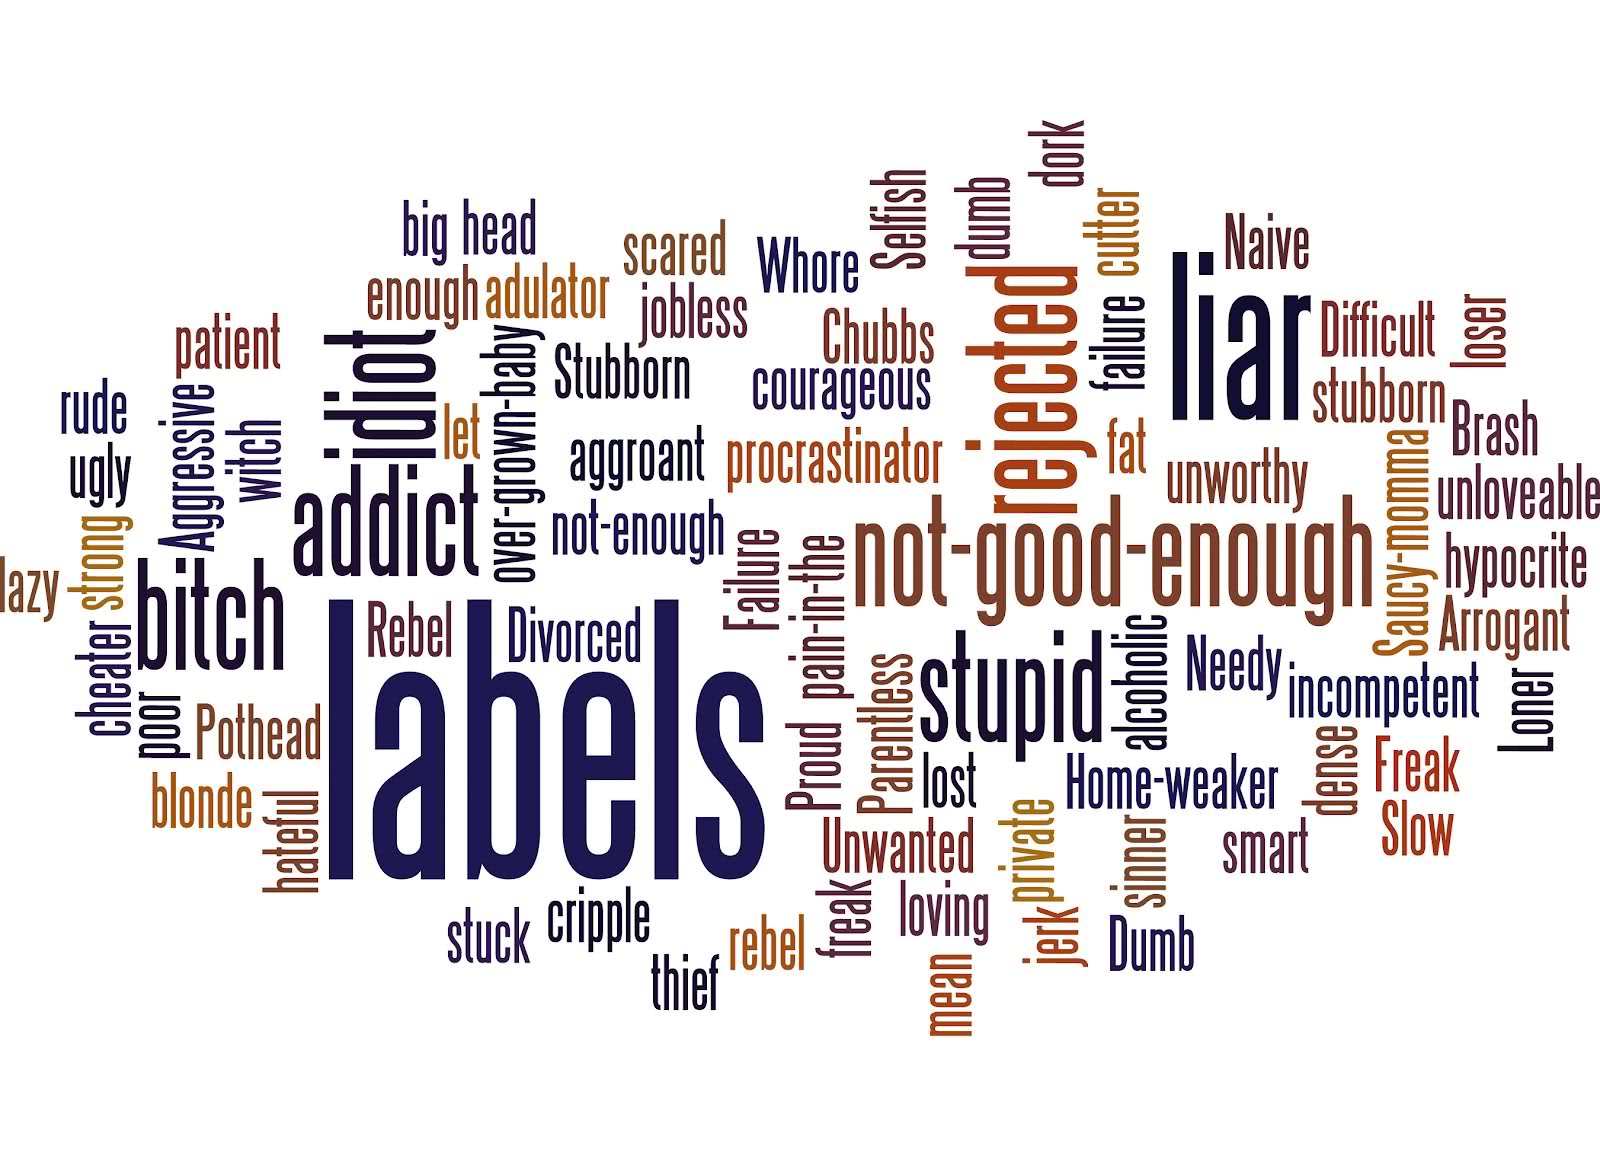
\includegraphics[height=6.5cm,width=9cm]{./Images/labels}

\huge

\pause
$\textcolor{red}{\Diamond \exists x G(x)^{\textcolor{Blue}{\text{\colorbox{yellow!50}{worldlabel}}}}}$
\hfill $\longrightarrow$ \hfill
$\textcolor{Blue}{(\textcolor{red}{(\Diamond \exists x G(x))_{\worldtype \typearrow o}
  \, {\textcolor{Blue}{\text{worldlabel}_\mu}}})}$
\end{frame}

\begin{frame}[t]{Advantage: \textcolor{red}{5. Relation to standard
      translation}}
{extra-logical translation vs. extended intra-logical translation
  (here)}  

\ \hfill  \chriscite{Benzm{\"u}llerPaulson, LogicaUniversalis, 2013}

\ \hfill  \chriscite{Benzm{\"u}llerWoltezenlogelPaleo, ECAI, 2014}

\vskip1em

\begin{block}{Intra-logical realisation of the standard translation}
\Large
$\phantom{\longrightarrow \qquad} \textcolor{red}{(\Box \phi)^{\textcolor{Blue}{\text{\colorbox{yellow!50}{a}}}}}$ 

\pause
$\longrightarrow \qquad \textcolor{Blue}{(\textcolor{red}{(\Box \phi)
    _{\worldtype \typearrow o}}\, a)}$ 

\pause
$\longrightarrow \qquad \textcolor{Blue}{(\textcolor{red}{(\textcolor{Blue}{ 
      (\lambda{\varphi_{\worldtype\typearrow o}} \lambda{w_\worldtype}
      \forall {u_\worldtype}\, (\neg r w u \vee
      \varphi u))}\, \phi)_{\worldtype \typearrow o}}\, a)}$ 

\pause
$\longrightarrow \qquad \textcolor{Blue}{(\textcolor{Blue}{ 
      \forall {u_\worldtype}\, (\neg r a u \vee
      \textcolor{red}{\phi_{\worldtype \typearrow o}}\, u)}}$ 
\end{block}

\vskip2em \pause
\begin{block}{We have extended this also for first-order and
    higher-order quantifiers!} \Large
$\phantom{\longrightarrow \qquad} \textcolor{red}{(\forall x\,
  \phi(x))^{\textcolor{Blue}{\text{\colorbox{yellow!50}{a}}}}}$ 

\pause
$\longrightarrow \qquad \textcolor{Blue}{(\textcolor{red}{(\forall x\,
    \phi(x))
    _{\worldtype \typearrow o}}\, a)}$ 

\pause
$\longrightarrow \qquad \textcolor{Blue}{(\textcolor{red}{(\forall (\lambda x\,
    \phi(x)))_{\worldtype \typearrow o}}\, a)}$ 

\pause
$\longrightarrow \qquad \textcolor{Blue}{(\textcolor{red}{(\textcolor{Blue}{ 
      (\lambda{h_{\gamma\typearrow(\worldtype \typearrow o)}}
      \lambda{w_\worldtype} \forall {d_\gamma} \, h d w)} (\lambda x\,
    \phi(x)))_{\worldtype \typearrow o}}\, a)}$ 

\pause
$\longrightarrow \qquad \textcolor{Blue}{\forall {d} \, (\textcolor{red}{\phi(d) _{\worldtype \typearrow o}}\, a)}$
\end{block}


\end{frame}


\begin{frame}{Advantage: \textcolor{red}{6. Meta-logical reasoning}}
{various examples already exist, e.g. verification of modal logic
  cube}
\ \hfill \chriscite{Benzm\"uller, FestschriftWalther, 2010} \\
\ \hfill \chriscite{Benzm{\"u}llerClausSultana, PxTP, 2015}
\vskip1em

		\scalebox{0.6}{
		\begin{tikzpicture}[thick,node/.style={rectangle,draw,font=\Large\bfseries}]

		  % 1. Ebene
		  \node[node] (K)   {K};
		  \node[node] (K4)  [above right=2cm and 2cm of K.center,anchor=center] {K4};
		  \node[node] (K5)  [below right=0.9cm and 1.6cm of K4.center,anchor=center] {K5};
		  \node[node] (KB)  [right=8cm of K.center,anchor=center] {KB};
		  \node[node] (K45) [right=5cm of K4.center,anchor=center] {K45};
		  \node[node] (KB5) [above right=2cm and 2cm of KB.center,anchor=center] {KB5};

		  % 2. Ebene
		  \node[node] (D)  [above=4cm of K.center,anchor=center] {D};
		  \node[node] (D4) [above right=2cm and 2cm of D.center,anchor=center] {D4};
		  \node[node] (D5) [below right=0.9cm and 1.6cm of D4.center,anchor=center] {D5};
		  \node[node] (DB) [right=8cm of D.center,anchor=center] {DB};
		  \node[node] (D45)[right=5cm of D4.center,anchor=center] {D45};

		  % 3. Ebene
		  \node[node] (M)  [above=4cm of D.center,anchor=center] {M};
		  \node[node] (S4) [above right=2cm and 2cm of M.center,anchor=center] {S4};
		  \node[node] (B)  [right=8cm of M.center,anchor=center] {B};
		  \node[node] (B)  [right=8cm of M.center,anchor=center] {B};
		  \node[node] (S5) [above right=2cm and 2cm of B.center,anchor=center] {S5};

		  \node[align=center,font=\Large\bfseries] [right=0.1cm of S5.north east,anchor=north west]
		   {\begin{tabular}{ l }
			 $\equiv$ M5 $\equiv$ MB5 $\equiv$ M4B5\\
			 $\equiv$ M45 $\equiv$ M4B $\equiv$ D4B\\
			 $\equiv$ D4B5 $\equiv$ DB5
			\end{tabular}
			};
		  \node[align=left,font=\large\bfseries] [above right=1.75cm and 3cm of D45.north east,anchor=north west]
		   {
		   \begin{tabular}{ l l }
			  M: & $\nec P \rightarrow P$ \\
			  B: & $P \rightarrow \nec\pos P$ \\
			  D: & $\nec P \rightarrow \pos P$ \\
			  4: & $\nec P \rightarrow \nec\nec P$ \\
			  5: & $\pos P \rightarrow \nec\pos P$
		   \end{tabular}
		   };

		  \node[draw=none,fill=none,font=\large\bfseries] (K1) [below right=2.5cm and 3.25cm of D45.south east,anchor=north west] {K};
		  \node[draw=none,fill=none,font=\large\bfseries] (M1) [above=2cm of K1.center,anchor=center] {M};
		  \node[draw=none,fill=none,font=\large\bfseries] (41) [above right=1.25cm and 1.25cm of K1.center,anchor=center] {4};
		  \node[draw=none,fill=none,font=\large\bfseries] (51) [above right=0.75cm and 1.75cm of K1.center,anchor=center] {5};
		  \node[draw=none,fill=none,font=\large\bfseries] (B1) [right=2cm of K1.center,anchor=center] {B};
		   
		  \node[align=center,font=\Large\bfseries] [right=0.1cm of KB5.north east,anchor=north west]
		   {$\equiv$ K4B5 $\equiv$ K4B};
		  \path[->,>=stealth',thick,every node/.style={font=\large}]
			(K1)  edge (M1)
				  edge (41)
				  edge (51)
				  edge (B1);

		  \path[->,>=stealth',thick,every node/.style={font=\large}]
			(K)   edge (K4)
				  edge (K5)
				  edge (KB)
				  edge (D)
			(K4)  edge (K45)
				  edge (D4)
			(K5)  edge (K45)
				  edge (D5)
			(KB)  edge (KB5)
				  edge (DB)
			(K45) edge (KB5)
				  edge (D45)
			(KB5) edge (S5)

			(D)   edge (D4)
				  edge (D5)
				  edge (DB)
				  edge (M)
			(D4)  edge (D45)
				  edge (S4)
			(D5)  edge (D45)
			(DB)  edge (B)
			(D45) edge (S5)

			(M)  edge (S4)
				 edge (B)
			(S4) edge (S5)
			(B)  edge (S5);
			
		\end{tikzpicture}
		}

\ \hfill \textcolor{red}{Verification of cube in less than 1 minute in Isabelle/HOL}
\end{frame}

\begin{frame}{Advantage: \textcolor{red}{7. Direct calculi and user intuition}}
{abstract level tactics (here in Coq) on top of embedding, hiding of embedding}
\ \hfill \chriscite{Benzm\"ullerWoltzenlogelPaleo, CSR'2015}

\fbox{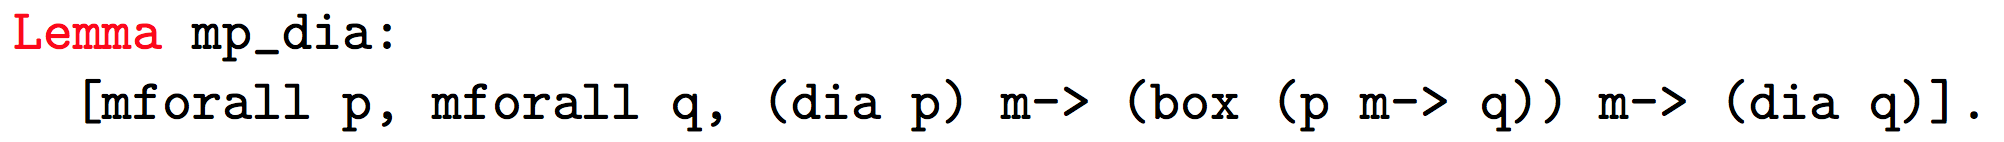
\includegraphics[width=\textwidth]{Images/CoqCode/10.png}}\\[.5em]
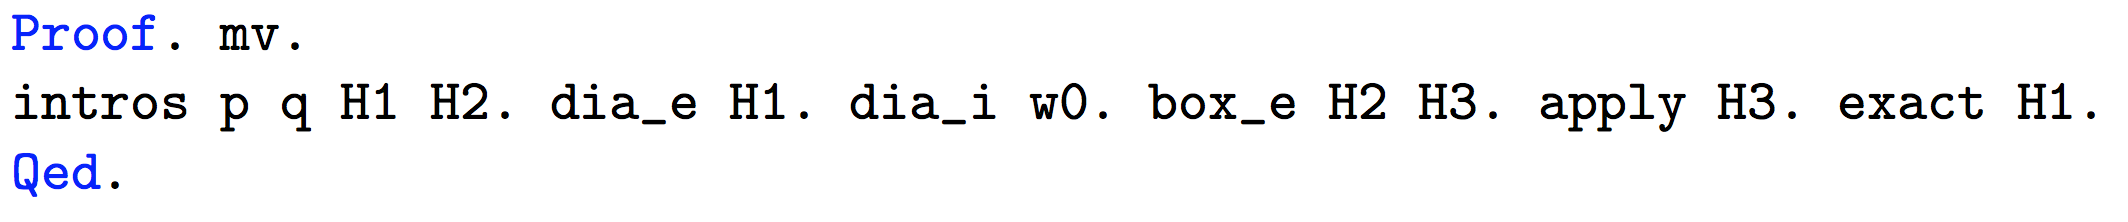
\includegraphics[width=\textwidth]{Images/CoqCode/13.png}

\begin{center}
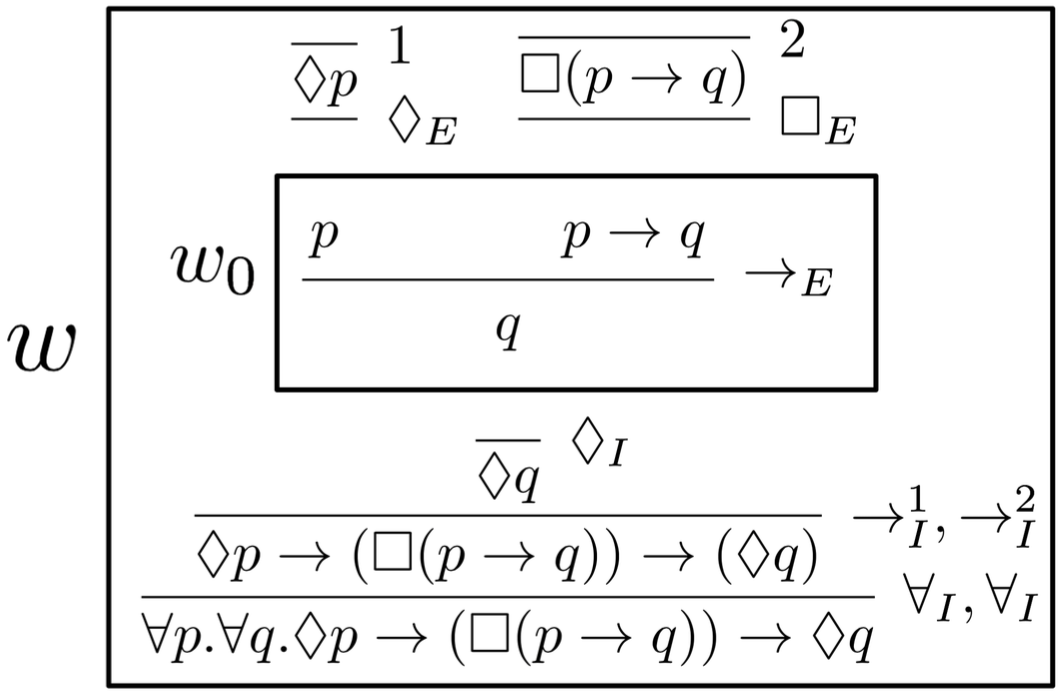
\includegraphics[width=0.65\textwidth]{Images/CoqCode/MP_Dia.png}
\end{center}
\end{frame}

\begin{frame}[t]{Advantage: \textcolor{red}{8. Soundness and completeness}}
{already proven for many non-classical logics (wrt Henkin semantics)}
\begin{block}{Soundness and Completeness \onslide*<0>{(and Cut-elimination)}}
\qquad
  $\models^{\textcolor{red}{L}} {\textcolor{red}{\varphi}} \quad
  \text{iff}\quad \text{\textcolor{Blue}{Ax}} \models^{{\textcolor{Blue}{HOL}}}_{{\text{\tiny \textcolor{Blue}{Henkin}}}}
  \textcolor{brown}{valid}\, {\textcolor{red}{\varphi_{\worldtype\typearrow o}}} \quad
  {\onslide*<0>{ ( \text{iff} \quad  \text{\textcolor{Blue}{Ax}} \vdash^{\text{{\textcolor{Blue}{HOL}}}}_{{\textcolor{Blue}{\text{cut-free}}}}
      \textcolor{brown}{valid}\, {\textcolor{red}{\varphi_{\worldtype\typearrow o}}} ) }}$
\end{block}
%\small
\vskip1em
Logic {\textcolor{red}{L}}:
\begin{itemize}
\item {\textcolor{red}{Higher-order  Modal Logics}} \hfill
  \chriscite{Benzm{\"u}llerWoltezenlogelPaleo, ECAI, 2014}\\

\item {\textcolor{red}{First-order  Multimodal Logics}} \hfill
  \chriscite{Benzm{\"u}llerPaulson, LogicaUniversalis, 2013}\\
\item {\textcolor{red}{Propositional Multimodal Logics} \hfill \chriscite{Benzm{\"u}llerPaulson, Log.J.IGPL, 2010}}\\

\item {\textcolor{red}{Quantified Conditional Logics} \hfill
  \chriscite{Benzm{\"u}ller, IJCAI, 2013}}  \\
\item {\textcolor{red}{Propositional Conditional Logics} \hfill
  \chriscite{Benzm{\"u}llerEtAl., AMAI, 2012}} \\

\item {\textcolor{red}{Intuitionistic Logics}  \hfill \chriscite{Benzm{\"u}llerPaulson, Log.J.IGPL, 2010}} \\

\item {\textcolor{red}{Access Control Logics}  \hfill \chriscite{Benzm{\"u}ller, IFIP SEC, 2009}} \\

\item {\textcolor{red}{Logic Combinations}  \hfill \chriscite{Benzm{\"u}ller, AMAI, 2011}} \\

%\item {\textcolor{red}{Ontologies: SUMO, DOLCE, OWL-full}}

\item \ldots more is on the way \ldots\ including: 
\begin{itemize}
   \item \textcolor{red}{Description Logics}
   \item \textcolor{red}{Nominal Logics}
   \item \textcolor{red}{Multivalued Logics (SIXTEEN)}
   \item \textcolor{red}{Logics based on Neighborhood Semantics}
   \item \textcolor{red}{(Mathematical) Fuzzy Logics}
   \item \textcolor{red}{Paraconsistent Logics}
\end{itemize}
\end{itemize}
\end{frame}

\begin{frame}[t]{Advantage: \textcolor{red}{9. Cut-elimination}}
{generic indirect result, since HOL enjoys cut-elimination (Henkin
  semantics)}
\begin{block}{Soundness and Completeness \onslide*<2->{and Cut-elimination}}
\qquad
  $\models^{\textcolor{red}{L}} {\textcolor{red}{\varphi}} \quad
  \text{iff}\quad \text{\textcolor{Blue}{Ax}} \models^{{\textcolor{Blue}{HOL}}}_{{\text{\tiny \textcolor{Blue}{Henkin}}}}
  \textcolor{brown}{valid}\, {\textcolor{red}{\varphi_{\worldtype\typearrow o}}} \quad
  {\onslide*<2->{ \text{iff} \quad  \text{\textcolor{Blue}{Ax}} \vdash^{\text{{\textcolor{Blue}{HOL}}}}_{{\textcolor{Blue}{\text{cut-free}}}}
      \textcolor{brown}{valid}\, {\textcolor{red}{\varphi_{\worldtype\typearrow o}}} }}$
\end{block}
%\small
\onslide*<1-2>{
\vskip1em
Logic {\textcolor{red}{L}}:
\begin{itemize}
\item {\textcolor{red}{Higher-order  Modal Logics}} \hfill
  \chriscite{Benzm{\"u}llerWoltezenlogelPaleo, ECAI, 2014}\\

\item {\textcolor{red}{First-order  Multimodal Logics}} \hfill
  \chriscite{Benzm{\"u}llerPaulson, LogicaUniversalis, 2013}\\
\item {\textcolor{red}{Propositional Multimodal Logics} \hfill \chriscite{Benzm{\"u}llerPaulson, Log.J.IGPL, 2010}}\\

\item {\textcolor{red}{Quantified Conditional Logics} \hfill
  \chriscite{Benzm{\"u}ller, IJCAI, 2013}}  \\
\item {\textcolor{red}{Propositional Conditional Logics} \hfill
  \chriscite{Benzm{\"u}llerEtAl., AMAI, 2012}} \\

\item {\textcolor{red}{Intuitionistic Logics}  \hfill \chriscite{Benzm{\"u}llerPaulson, Log.J.IGPL, 2010}} \\

\item {\textcolor{red}{Access Control Logics}  \hfill \chriscite{Benzm{\"u}ller, IFIP SEC, 2009}} \\

\item {\textcolor{red}{Logic Combinations}  \hfill \chriscite{Benzm{\"u}ller, AMAI, 2011}} \\

%\item {\textcolor{red}{Ontologies: SUMO, DOLCE, OWL-full}}

\item \ldots more is on the way \ldots\ including: 
\begin{itemize}
   \item \textcolor{red}{Description Logics}
   \item \textcolor{red}{Nominal Logics}
   \item \textcolor{red}{Multivalued Logics (SIXTEEN)}
   \item \textcolor{red}{Logics based on Neighborhood Semantics}
   \item \textcolor{red}{(Mathematical) Fuzzy Logics}
   \item \textcolor{red}{Paraconsistent Logics}
\end{itemize}
\end{itemize}
}

\onslide*<3>{
\begin{center}
\colorbox{gray!20}{
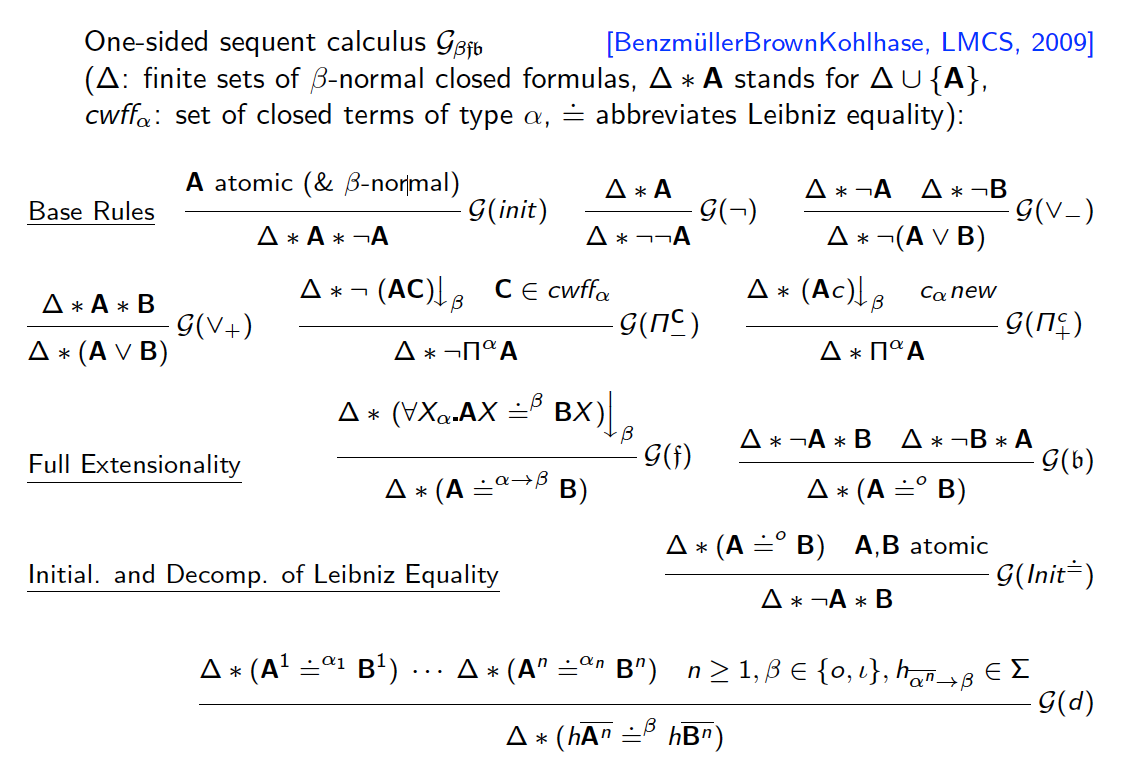
\includegraphics[width=.8\linewidth]{./Images/Varia/HOLCutFreeSequentCalculus.png}
}
\end{center}
}
\end{frame}

% \ \hfill \chriscite{Benzm\"ullerWoltzenlogelP., RW'2015, CSR'2015,
%   ECAI'2014, WADT'2014, AFP'2013} \\
% \ \hfill \chriscite{Benzm\"ullerPaulson, Logica Universalis, 2013} \\
% \ \hfill \chriscite{Benzm\"uller, IJCAI'2013} \\[2em]




\begin{transitionframe}{./Images/Transitions/ComputerCross}{black}%$
  \centering
 \textbf{Part B: \\ HOL ATP's (in particular LEO-II) contributed \\ New Knowledge in Metaphysics}
 %\\ into Higher-Order Logic}
 %\textbf{Embedding Higher-Order Modal Logic \\ into Higher-Order
 %Logic}
\end{transitionframe}



\begin{frame}{Vision of Leibniz (1646--1716): \textit{Calculemus!}}
\begin{changemargin}{-.5cm}{-.5cm}
\begin{minipage}{4cm}
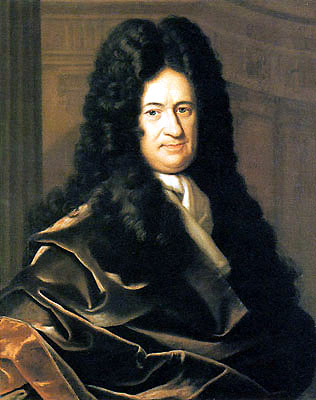
\includegraphics[width=4cm]{./Images/Varia/Leibniz.png} 

\vspace*{1em}
\color{gray}\footnotesize
If controversies were to arise, there would be no more need of
disputation between two philosophers than between two
accountants. For it would suffice to take their pencils in their
hands, to sit down to their slates, and to say to each other \ldots :
Let us calculate. \\ \phantom{bla} \, \hfill (Translation by Russell)
\end{minipage} \hfill
\begin{minipage}{7cm} \small
Quo facto, quando orientur controversiae, non magis disputatione opus erit inter
duos philosophos, quam inter duos Computistas. Sufficiet enim calamos in
manus sumere sedereque ad abacos, et sibi mutuo \ldots dicere: calculemus.
\hfill (Leibniz, 1684)
\vspace*{1em}

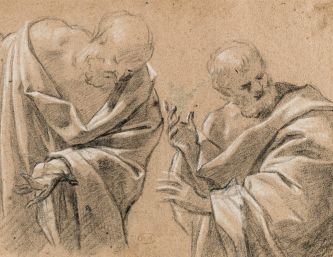
\includegraphics[width=7cm,height=5cm]{./Images/Varia/Dispute1.jpg}

\vspace*{1em}
Required: \\
\, \hfil \textbf{characteristica universalis} and  \textbf{calculus ratiocinator}
\end{minipage}
\end{changemargin}
\end{frame}


\begin{frame}[t]{Our Contribution: Towards Computational Metaphysics}
\large
\vskip2em
\begin{block}{Ontological argument for the existence of God} 
\begin{itemize}
\item {Focus on G\"odel's modern version in higher-order modal logic} \\[.5em]
\item {Experiments with HO provers and embedding approach} \\[.5em]
\end{itemize}
\end{block}
\pause

\vfill

\begin{block}{Different interests in ontological arguments} 
\begin{itemize}
\item \textcolor{Blue}{Philosophical:} Boundaries of metaphysics \& epistemology
 %  \begin{itemize}
 %  \item We specify a metaphysical concept (God), 
 %  \item but we want to draw
 %      a conclusion for the real world. % \\[1em]
 % % \item Necessary Existence: metaphysical NE vs. logical NE  vs. modal NE 
   \\[.5em]
 % \end{itemize} 
\item \textcolor{Blue}{Theistic:} Successful argument could convince
  atheists? \\[.5em]
\item \textcolor{red}{Ours:} Computational metaphysics (Leibniz'
  vision) 
\end{itemize}
\end{block}
% \\[.5cm]
  % %\begin{itemize}
  % %\item 
  %   \ldots to formalize the definitions, axioms and theorems? \\
  % %\item 
  %   \ldots to verify/falsify the arguments step-by-step? \\
  % %\item 
  %   \ldots to automate (sub-)arguments? \\
  % %\item 
  %   \ldots to generate new knowledge?
  %\end{itemize}
  % \textcolor{red}{\emph{``Computer-assisted Theoretical Philosophy''}}\\[1em]
  %                                      remember Leibniz' dictum --- \emph{Calculemus!}
\end{frame}



% % \begin{frame}{Introduction -- Ontological Argument}\large
% % %Ontological argument: Conclude that God exists from premises by pure, a priori reasoning.
% % \begin{block}{Def: Ontological Argument}
% % \begin{itemize}
% % \item deductive argument 
% % \item for the existence of God 
% % \item starting from premises, which are justified by pure reasoning,
% % i.e. they do not depend on observation of the world.
% % \end{itemize}
% % \end{block}

% % \vfill \pause
% % \begin{block}{Existence of God: different types of arguments/proofs}
% % \begin{itemize}
% % \item[---]a posteriori (use experience/observation in the world)
% %   \begin{itemize}
% %   \item[------]teleological
% %   \item[------]cosmological
% %   \item[------]moral
% %   \item[------] \ldots
% %   \end{itemize}  
% % \item[---]a priori (based on pure reasoning, independent)
% %   \begin{itemize}
% %   \item[------]\textcolor{Blue}{ontological argument}
% %     \begin{itemize}
% %     \item[------]definitional 
% %     \item[------]modal 
% %     \item[------] \ldots
% %     \end{itemize}
% %   \item[------]other a priori arguments
% %   \end{itemize}
% % \end{itemize}
% % \end{block}
% % \end{frame}



\begin{frame}{A Long History}{\textcolor{Blue}{pros} and \textcolor{red}{cons}} \Large
\begin{changemargin}{-.2cm}{0cm}
\hskip-.5em
\ldots\rotatebox[origin = bl,width = 0mm]{65}{\textcolor{Blue}{Anselm v. C.}} \hskip-2.3em
          \rotatebox[origin = bl]{65}{\textcolor{red}{Gaunilo}} \hskip-1.3em
\ldots  \rotatebox[origin = bl]{65}{\textcolor{red}{Th. Aquinas}}  \hskip-2.3em
\ldots\ldots   \rotatebox[origin = bl]{65}{\textcolor{Blue}{Descartes}} \hskip-1.7em
               \rotatebox[origin = bl]{65}{\textcolor{Blue}{Spinoza}} \hskip-1.3em
               \rotatebox[origin = bl]{65}{\textcolor{Blue}{Leibniz}}  \hskip-1.2em
\ldots  \rotatebox[origin = bl]{65}{\textcolor{red}{Hume}}  \hskip-1em
          \rotatebox[origin = bl]{65}{\textcolor{red}{Kant}}  \hskip-.8em
\ldots  \rotatebox[origin = bl]{65}{\textcolor{Blue}{Hegel}}  \hskip-1.3em
\ldots  \rotatebox[origin = bl]{65}{\textcolor{red}{Frege}}  \hskip-1.3em
\ldots  \rotatebox[origin = bl]{65}{\textcolor{Blue}{Hartshorne}} \hskip-1.9em
          \rotatebox[origin = bl]{65}{\textcolor{Blue}{Malcolm}}  \hskip-1.4em
          \rotatebox[origin = bl]{65}{\textcolor{red}{Lewis}}  \hskip-1em
          \rotatebox[origin = bl]{65}{\textcolor{Blue}{Plantinga}}  \hskip-1.6em
          \rotatebox[origin = bl]{65}{\textcolor{Blue}{G\"odel}}   \hskip-1.2em
\ldots \\[1em]


\onslide<1->
{
\vfill
Anselm's notion of God (Proslogion, 1078):\\
\,\hfill \textbf{``God is that, than which nothing greater can be
  conceived.''} \\[1em]
}

\onslide<2->
{
G\"odel's notion of God:\\
\,\hfill \textbf{``A God-like being possesses all `positive'
  properties.''} \\[1em]
}

\onslide<1->
{
To show by logical, deductive reasoning: \\
\,\hfill \textbf{``\alt<2>{Necessarily, God exists.}{God exists.}''} \\
\,\hfill \alt<2>{${\nec} \exq x G(x)$}{$\exq x G(x)$}\\[1em]
}
\end{changemargin}
\end{frame}








% % \begin{frame}{The Ontological Proof Today}
% % \vskip1em
% % % \emph{\huge Wohl eine jede Philosophie kreist um den ontologischen
% % %   Gottesbeweis} \\[1.5em]
% % % (Adorno, Negative Dialektik, 1966)
% % % \vfill
% % \begin{center}

% % \hfill
% % 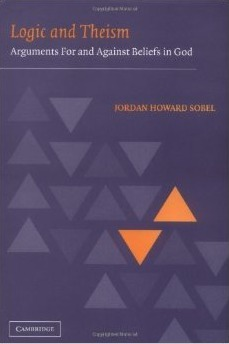
\includegraphics[height=2cm]{./Images/Books/buch3.jpg} \hfill
% % 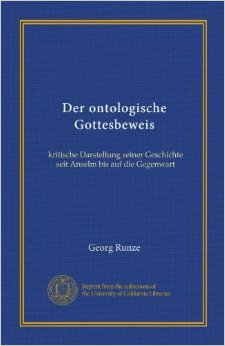
\includegraphics[height=2cm]{./Images/Books/buch2.jpg} \hfill 
% % 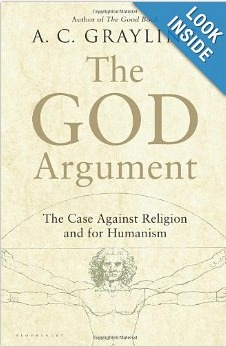
\includegraphics[height=2cm]{./Images/Books/buch4.jpg} \hfill
% % \hfill

% % \vspace{0.5 cm}

% % \hfill
% % 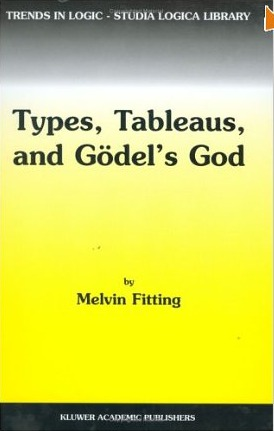
\includegraphics[height=2cm]{./Images/Books/buch7.jpg} \hfill
% % 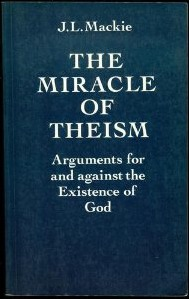
\includegraphics[height=2cm]{./Images/Books/buch5.jpg} \hfill
% % 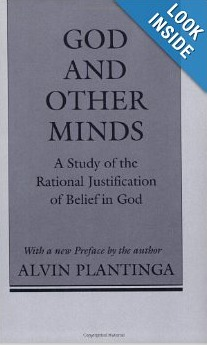
\includegraphics[height=2cm]{./Images/Books/buch6.jpg} \hfill
% % 
\includegraphics[height=2cm]{./Images/Books/buch1.jpg} \hfill
% % \hfill

% % \vspace{0.5 cm}

% % \hfill
% % 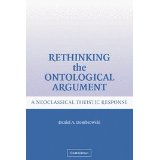
\includegraphics[height=2cm]{./Images/Books/buch8.jpg} \hfill
% % 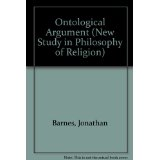
\includegraphics[height=2cm]{./Images/Books/buch9.jpg} \hfill
% % 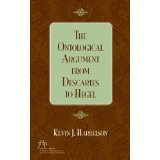
\includegraphics[height=2cm]{./Images/Books/buch10.jpg} \hfill
% % 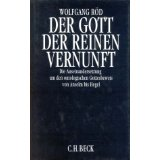
\includegraphics[height=2cm]{./Images/Books/buch11.jpg} \hfill
% % \hfill

% % \end{center}
% % See also our collection of recent papers: \\ {\small \url{https://github.com/FormalTheology/GoedelGod/tree/master/Literature}}
% % \end{frame}



\def\scottproofsimple{
\resizebox{\textwidth}{!}{
\begin{minipage}{12cm}%\small
\begin{itemize}
\item[Axiom A1] Either a property or its negation is positive, but not
  both: \hfill 
  ${\alt<0>{\textcolor{red}{\allq \phi}}{\allq \phi} [P(\neg \phi) \biimp \neg P(\phi)]}$ 
\item[Axiom A2] A property necessarily implied by a
  positive property is positive:  \phantom{bla bla bla bla bla bla bla}  \hfill 
  ${\alt<0>{\textcolor{red}{\allq \phi \allq \psi}}{\allq \phi \allq \psi} [(P(\phi) \wedge \alt<0>{\textcolor{red}{\nec}}{\nec} \allq x [\phi(x)
  \imp \psi(x)]) \imp P(\psi)]}$ 
\item[\textcolor{Green}{Thm. T1}] \textcolor{Green}{Positive properties are possibly exemplified:} \hfill \textcolor{Green}{${\alt<0>{\textcolor{red}{\allq \phi}}{\allq \phi} [P(\phi) \imp \alt<0>{\textcolor{red}{\pos}}{\pos}  \exq x \phi(x)]}$}
\item[Def. D1] A \emph{God-like} being possesses all positive properties: \hfill
  ${G(x) \biimp \alt<0>{\textcolor{red}{\allq \phi}}{\allq \phi} [P(\phi) \imp \phi(x)]}$ 
\item[Axiom A3]  The property of being God-like is positive: \hfill   ${P(G)}$ 
\item[\textcolor{Green}{Cor. C\phantom{1}}] \textcolor{Green}{Possibly, God exists:}\hfill \textcolor{Green}{${\alt<0>{\textcolor{red}{\pos}}{\pos} \exq x G(x)}$}
\item[Axiom A4]  Positive properties are necessarily positive: \hfill 
  ${\alt<0>{\textcolor{red}{\allq \phi}}{\allq \phi} [P(\phi) \imp \alt<0>{\textcolor{red}{\nec}}{\nec} P(\phi)]}$ 
\item[Def. D2] An \emph{essence} of an individual is a property possessed by it and necessarily implying any of its properties: \hfill ${\ess{\phi}{x} \biimp \alt<0>{\textcolor{red}{\phi(x)\,\wedge\,}}{\phi(x)\,\wedge\,}\alt<0>{\textcolor{red}{\allq \psi}}{\allq \psi} (\psi(x) \imp \alt<0>{\textcolor{red}{\nec}}{\nec} \allq y (\phi(y) \imp \psi(y)))}$ 
\item[\textcolor{Green}{Thm. T2}]  \textcolor{Green}{Being God-like is an essence of any
  God-like being:}  \hfill \textcolor{Green}{${\allq x [G(x) \imp \ess{G}{x}]}$}
\item[Def. D3] \emph{Necessary existence} of an individual~is the necessary exemplification of all its essences: 
  \phantom{b} \hfill ${\NE(x) \biimp \alt<0>{\textcolor{red}{\allq \phi}}{\allq \phi} [\ess{\phi}{x} \imp \alt<0>{\textcolor{red}{\nec}}{\nec}  \exq y \phi(y)]}$
\item[Axiom A5] Necessary existence is a positive property: \hfill ${P(\NE)}$ 
\item[\textcolor{Green}{Thm. T3}] \textcolor{Green}{Necessarily, God exists:} \hfill \textcolor{Green}{${\alt<0>{\textcolor{red}{\nec}}{\nec} \exq x G(x)}$}
\end{itemize}
\end{minipage}
}}


\usebackgroundtemplate{
  \vbox to \paperheight{\vfil\hbox to \paperwidth{\hfil
      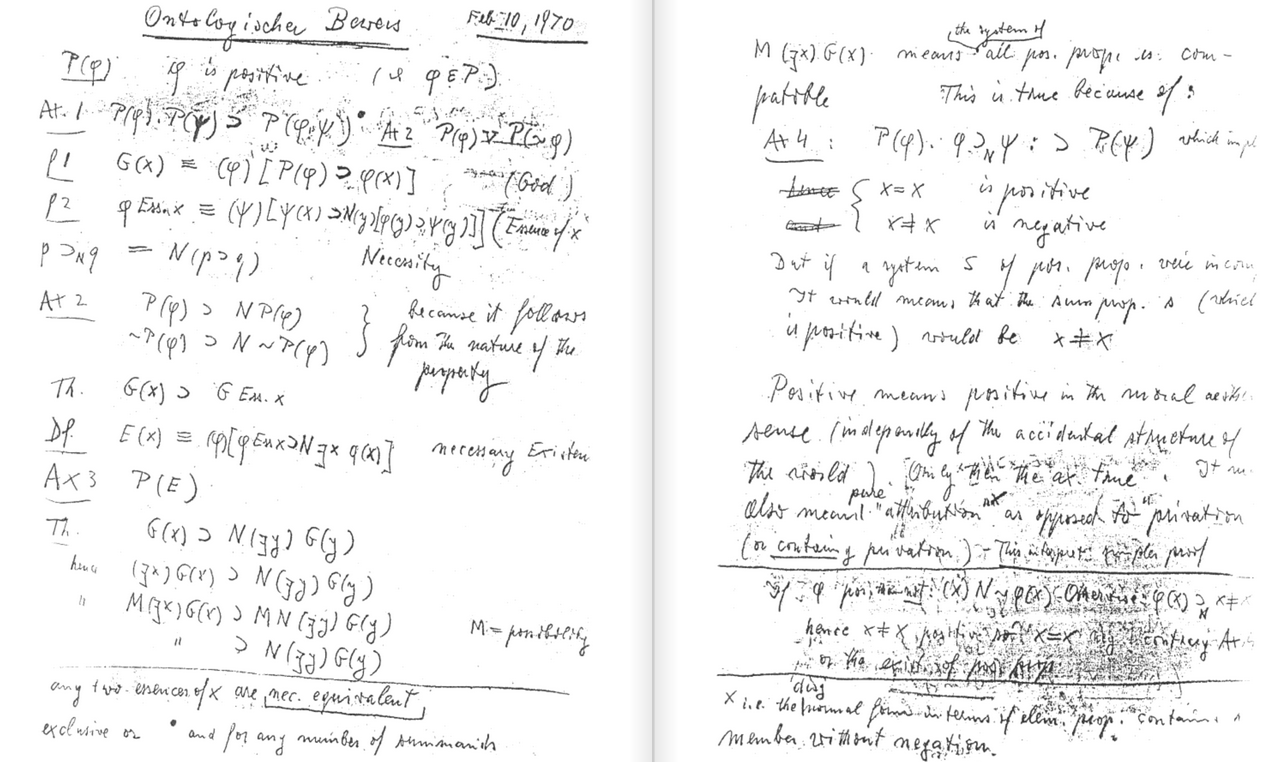
\includegraphics[width=12.5cm]{./Images/Manuscript.png} 
      \hfil}\vfil}
}
\begin{frame}{G\"odel's Manuscript: 1930's, 1941, 1946-1955, 1970}
\end{frame}
\usebackgroundtemplate{}


\begin{frame}{Scott's Version of G\"odel's Axioms, Definitions and
    Theorems}
\begin{changemargin}{-.2cm}{.5cm}
\begin{pgfpicture}{0cm}{0cm}{11cm}{11cm}
\pgfsetlinewidth{5\pgflinewidth} 
%\pgfsetendarrow{\pgfarrowto}
%\pgfsetstartarrow{\pgfarrowto}
%\pgfnodecircle{Node1}[stroke]{\pgfxy(0,9.5)}{0.25cm}
\pgfnodebox{Node0}[virtual]{\pgfxy(6,7.5)}{\begin{minipage}{11.5cm} \scottproofsimple\end{minipage}}{.2cm}{.2cm}
\end{pgfpicture}
\end{changemargin}
\end{frame}

\begin{frame}{Scott's Version of G\"odel's Axioms, Definitions and
    Theorems}
\begin{changemargin}{-.2cm}{-.5cm}
\begin{pgfpicture}{0cm}{0cm}{11cm}{11cm}
\pgfsetlinewidth{4\pgflinewidth} 
%\pgfsetendarrow{\pgfarrowto}
%\pgfsetstartarrow{\pgfarrowto}
%\pgfnodecircle{Node1}[stroke]{\pgfxy(0,9.5)}{0.25cm}
\pgfnodebox{Node0}[virtual]{\pgfxy(6,7.5)}{\begin{minipage}{11.5cm} \scottproofsimple\end{minipage}}{.2cm}{.2cm}
\pgfnodebox{Node1}[stroke]{\pgfxy(7.2,6.6)}{\phantom{B}}{.4cm}{.2cm}
\pgfnodebox{Node2}[virtual]{\pgfxy(7,3.5)}{
\framecolorbox[8.5cm][s]{Blue}{Blue!20}{
\begin{minipage}{8cm}\color{black} 
\vskip1em
\begin{center} Difference to G\"odel (who omits this conjunct) \end{center}
\phantom{bla}
\end{minipage}
}}{0pt}{0pt}
\pgfnodeconncurve{Node1}{Node2}{300}{120}{1cm}{1cm}
\end{pgfpicture}
\end{changemargin}
\end{frame}



\begin{frame}{Scott's Version of G\"odel's Axioms, Definitions and
    Theorems}
\begin{changemargin}{-.2cm}{-.5cm}
\begin{pgfpicture}{0cm}{0cm}{11cm}{11cm}
\pgfsetlinewidth{4\pgflinewidth} 
%\pgfsetendarrow{\pgfarrowto}
%\pgfsetstartarrow{\pgfarrowto}
%\pgfnodecircle{Node1}[stroke]{\pgfxy(0,9.5)}{0.25cm}
\pgfnodebox{Node0}[virtual]{\pgfxy(6,7.5)}{\begin{minipage}{11.5cm} \scottproofsimple\end{minipage}}{.2cm}{.2cm}
\pgfnodebox{Node1}[stroke]{\pgfxy(8.2,9.8)}{\phantom{B}}{.15cm}{.15cm}
\pgfnodebox{Node2}[stroke]{\pgfxy(10.6,7.9)}{\phantom{B}}{.15cm}{.15cm}
\pgfnodebox{NodeX}[virtual]{\pgfxy(7,3.5)}{
\framecolorbox[8.5cm][s]{Blue}{Blue!20}{
\begin{minipage}{8cm}\color{black} 
\vskip1em
\begin{center} Modal operators are used \end{center}
\phantom{bla}
\end{minipage}
}}{0pt}{0pt}
\pgfnodeconncurve{Node1}{NodeX}{270}{120}{1cm}{1cm}
\pgfnodeconncurve{Node2}{NodeX}{270}{110}{1cm}{1cm}
\end{pgfpicture}
\end{changemargin}
\end{frame}




\begin{frame}{Scott's Version of G\"odel's Axioms, Definitions and
    Theorems}
\begin{changemargin}{-.2cm}{-.5cm}
\begin{pgfpicture}{0cm}{0cm}{11cm}{11cm}
\pgfsetlinewidth{4\pgflinewidth} 
%\pgfsetendarrow{\pgfarrowto}
%\pgfsetstartarrow{\pgfarrowto}
%\pgfnodecircle{Node1}[stroke]{\pgfxy(0,9.5)}{0.25cm}
\pgfnodebox{Node0}[virtual]{\pgfxy(6,7.5)}{\begin{minipage}{11.5cm} \scottproofsimple\end{minipage}}{.2cm}{.2cm}
\pgfnodebox{Node1}[stroke]{\pgfxy(6.55,9.8)}{\phantom{B}}{.4cm}{.15cm}
\pgfnodebox{Node2}[stroke]{\pgfxy(9.65,8.8)}{\phantom{B}}{.15cm}{.15cm}
\pgfnodebox{NodeX}[virtual]{\pgfxy(7,3.5)}{
\framecolorbox[8.5cm][s]{Blue}{Blue!20}{
\begin{minipage}{8cm}\color{black} 
\vskip1em
\begin{center} second-order quantifiers \end{center}
\phantom{bla}
\end{minipage}
}}{0pt}{0pt}
\pgfnodeconncurve{Node1}{NodeX}{180}{120}{1cm}{1cm}
\pgfnodeconncurve{Node2}{NodeX}{270}{110}{1cm}{1cm}
\end{pgfpicture}
\end{changemargin}
\end{frame}




% \usebackgroundtemplate{}
% \begin{frame}{Scott's Version of G\"odel's Axioms, Definitions and Theorems}
% \scottproof
% \end{frame}





\newcommand{\phantomCOne}{
\begin{prooftree}
\AXC{$\phantom{\textbf{A3}}$} \noLine
\UIC{$\phantom{P(G)}$}
		\AXC{$\phantom{\textbf{A2}}$} \noLine
		\UIC{$\phantom{\all \varphi. \all \psi.[(P(\varphi) \wedge \nec \all x.[\varphi(x) \imp \psi(x)]) \imp P(\psi)]}$}
					\AXC{$\phantom{\textbf{A1($\supset$)}}$} \noLine
					\UIC{$\phantom{\all \varphi. [P(\neg \varphi) \imp \neg P(\varphi)]}$} \noLine
				\BIC{$\phantom{\textbf{T1: } \all \varphi. [P(\varphi) \imp \pos \ex x.\varphi(x)]}$} \noLine
	\BIC{$\phantom{\textbf{C: } \pos \ex z. G(z)}$}
\end{prooftree}
}

\newcommand{\phantomTTwo}{
\begin{prooftree}
						\AXC{$\phantom{\textbf{A1b}}$} \noLine
						\UIC{$\phantom{\all \varphi. [\neg P(\varphi) \imp P(\neg \varphi)]}$}
								\AXC{$\phantom{\textbf{A4}}$} \noLine
								\UIC{$\phantom{ \all \varphi.[P(\varphi) \to \Box \; P(\varphi)]} $} \noLine
							\BIC{$\phantom{\textbf{T2: } \all y.[G(y) \imp \ess{G}{y}]}$}
									\AXC{$\phantom{\textbf{A5}}$} \noLine
									\UIC{$ \phantom{P(NE)} $} \noLine
								\BIC{$\phantom{\textbf{L1: } \ex z. G(z) \imp \nec \ex x. G(x)}$} \noLine
								\UIC{$\phantom{\pos \ex z. G(z) \imp \pos \nec \ex x. G(x)}$}
										\AXC{$\phantom{\textbf{S5}}$} \noLine
 										\UIC{$\phantom{\all \xi.[\pos \nec \xi \imp \nec \xi]}$} \noLine	
									\BIC{$\phantom{\textbf{L2: } \pos \ex z. G(z) \imp \nec \ex x. G(x)}$}
\end{prooftree}
}

\newcommand{\phantomDOne}{
$$
\phantom{
\textbf{D1: } G(x) \equiv \forall \varphi. [P(\varphi) \to \varphi(x)]}
$$
}

\newcommand{\DOne}{
$$
\textbf{D1: } G(x) \equiv \forall \varphi. [P(\varphi) \to \varphi(x)]
$$
}

\newcommand{\phantomDTwo}{
$$
\phantom{
\textbf{D2: } \ess{\varphi}{x} \equiv \varphi(x) \wedge \all \psi. (\psi(x) \imp \nec \all x. (\varphi(x) \imp \psi(x)))
}
$$
}

\newcommand{\DTwo}{
$$
\textbf{D2: } \ess{\varphi}{x} \equiv \textcolor{Blue}{\varphi(x)} \wedge \all \psi. (\psi(x) \imp \nec \all x. (\varphi(x) \imp \psi(x)))
$$
}


\newcommand{\phantomDThree}{
$$
\phantom{
\textbf{D3: } NE(x) \equiv \all \varphi.[\ess{\varphi}{x} \imp \nec \ex y.\varphi(y)]
}
$$
}

\newcommand{\DThree}{
$$
\textbf{D3: } NE(x) \equiv \all \varphi.[\ess{\varphi}{x} \imp \nec \ex y.\varphi(y)]
$$
}








% \begin{frame}{Proof Overview}
% Side result:
% \begin{itemize}
% \item new natural deduction calculus
% \item for higher-order modal logic
% \end{itemize}
% \end{frame}

% \begin{frame}{Proof Overview}
% Gödel proves God's necessary existence by first 
% proving that, if God's existence is at all possible, 
% then it must be necessary (Lemma L2). This idea is 
% already present in St. Anselm's and Descartes' 
% arguments. \\[1em]

% Leibniz argued that these arguments are 
% incomplete because they assumed the possibility of 
% God's existence (Corollary C1) without any proof. 
% For Leibniz, this should be derivable from the 
% definition of God as a perfect being and from the 
% notion of perfection. This idea can be clearly 
% recognized in Gödel's proof: from axioms A1 and A2, 
% one can derive that, for any positive property, 
% the existence of a being having this property is 
% possible (Theorem T1). \\[1em]

% As God is defined as a being 
% who possesses all positive properties, the property 
% of being God-like must be, by axiom A3, a positive 
% property as well.  C1 then follows trivially from T1.  \\[1em]

% The hardest lemmas in Gödel's
% proof are T2 and L2.  For that, Gödel had to formulate a non-trivial
% definition of "essence", in order not only to derive T2 from A1 and A4
% but also to state an arguably acceptable axiom A5 allowing the
% derivation of L2 from T2 and other axioms from the modal logic S5.
% \end{frame}



% \begin{transitionframe}{./Images/Transitions/ComputerCross}{black}%$
%   \centering
% \textbf{How to automate Higher-Order Modal Logic?}
% %\\ into Higher-Order Logic}
% %\textbf{Embedding Higher-Order Modal Logic \\ into Higher-Order Logic}
% \end{transitionframe}

% \begin{frame}{Embedding HOML in HOL} \large

%   \hskip-1em Challenge: \hfill No provers for \emph{\textcolor{red}{Higher-order Modal
%     Logic}\/} (\textcolor{red}{HOML}) \\[1em]

% \hskip-1em Our solution: \hfill Embedding in \textbf{\textcolor{Blue}{$\stackrel{\text{\normalsize Church's Simple Type Theory}}{\text{Higher-order Classical Logic}}$}} (\textcolor{Blue}{HOL})\\
% %\,\hfill \textbf{Church's Simple Type Theory (\phantom{HOL})} \\
% \, \hfill Then use existing \textcolor{Blue}{HOL} theorem provers for reasoning in \textcolor{red}{HOML} \\
% \,\hfill {\chriscite{Benzm\"ullerPaulson, Logica Universalis, 2013}}
% \\[2em]

% \hskip-1em Assumption:  
% \,\hfill Henkin semantics for both \textcolor{Red}{HOML} and
% \textcolor{Blue}{HOL} \\[2em]

% % \hskip-1em Previous empirical findings:  \\[.5em]
% % \,\hfill Embedding of  \textcolor{red}{\emph{First-order Modal Logic}} in \textcolor{Blue}{HOL} works well 

% % \,\hfill {\small [Benzm\"ullerOttenRaths, ECAI, 2012]} \\
% % \,\hfill {\small [Benzm\"uller, LPAR, 2013]} \\[2em]
% \end{frame}




% % \begin{frame}[t]{Classical Higher-Order Logic  (HOL)} \large

% % Simple Types \hfill $\alpha ::=  {o} \mid {\iota}
% % \mid \textcolor{gray}{\mu} \mid {\alpha_1 \typearrow \alpha_2}$\\[1em]
% % \textcolor{Blue}{\text{HOL}} \\[-3.2em]
% %  \begin{align*}
% %             \textcolor{Blue}{s},\textcolor{Blue}{t} ::=  & \textcolor{Blue}{C_{\alpha}} \mid \textcolor{Blue}{x_{\alpha}} \mid \textcolor{Blue}{(\lambda x_{\alpha}s_{\beta})_{\alpha \typearrow \beta}} \mid 
% %             \textcolor{Blue}{(s_{\alpha \typearrow \beta}\, t_\alpha)_{\beta}} \mid \\
% %             & \textcolor{Blue}{(\neg_{o \typearrow o}\;s_{o})_o} \mid \textcolor{Blue}{(s_o \vee_{o\typearrow o \typearrow o} t_o)_o}
% %             \mid \textcolor{Blue}{(\forall_{(\alpha \typearrow o)\typearrow o}\; s_{\alpha
% %               \typearrow o})_o}  \\[-1em]
% %           \end{align*}
% % \, \hfill \textcolor{gray}{(note:~binder~notation~\textcolor{Blue}{$\forall x_\alpha
% %             t_o$}~as~syntactic~sugar~for~\textcolor{Blue}{$\forall_{(\alpha
% %               \typearrow o)\typearrow o} \lambda x_\alpha t_o$})} \\[2em]

% % \pause

% % HOL with Henkin semantics is (meanwhile) well understood \\

% % \quad Origin, foundation for maths \hfill  \chriscite{Church,JSymbLog,1940} \\
% % \quad Henkin semantics \hfill \chriscite{Henkin,JSymb.Log,1950} \\
% %   \hfill \chriscite{Andrews, JSymbLog,1971,1972} \\
% % \quad Extensionality/Intensionality   \hfill \chriscite{Benzm\"ullerEtAl,JSymbLog,2004} \\
% % \, \hfill \chriscite{Muskens,JSymbLog,2007} \\[.5em]

% % \pause
% % Sound and complete provers do exists \\[.5em]
% %   \quad interactive: \hfill Isabelle/HOL, HOL4, Hol Light, Coq/HOL, PVS,
% %   \ldots \\[.5em]
% %   \quad automated: \hfill TPS, LEO-II, Satallax, Nitpick, Isabelle/HOL, \ldots \\

% % \end{frame}






% % \begin{frame}{Embedding HOML in HOL} \large
% % \begin{changemargin}{-.5cm}{0cm}

% % \textcolor{red}{HOML} \hfill
% % $\begin{array}{lll}\textcolor{red}{\varphi,\psi} & ::= &
% %   \textcolor{red}{\ldots}  \mid \textcolor{red}{\neg
% %     \varphi} \mid \textcolor{red}{\varphi \wedge \psi} \mid
% %   \textcolor{red}{\varphi \imp \psi}  \mid \textcolor{red}{\Box
% %     \varphi} \mid \textcolor{red}{\Diamond \varphi}  \mid
% %   \textcolor{red}{\forall {x_\gamma}\, \varphi} \mid
% %   \textcolor{red}{\exists {x_\gamma}\, \varphi} 
% % %\mid \textcolor{red}{\forall {P}\, \varphi} 
% % \end{array}$ \\[1em]


% % \begin{itemize}
% % \item Kripke style semantics (possible world semantics)\\
% % $\begin{array}{lcl} 
% % \onslide<1->{   \parbox[b]{2.5cm}{$M,g,s  \models  \textcolor{red}{ \neg \textcolor{black}{\varphi}}$}     & \text{ iff } &  \text{not } M,g,s \models {\varphi} \\}
% % \onslide<1->{   M,g,s  \models  \textcolor{red}{
% %     \textcolor{black}{\varphi} \wedge \textcolor{black}{\psi}}    &
% %   \text{ iff } &  M,g,s \models {\varphi} \text{ and } M,g,s \models
% %   {\psi} \\}
% % \ldots \\
% % \onslide<1->{   M,g,s  \models  \textcolor{red}{ \Box} \varphi & \text{ iff } &  M,g,u \models {\varphi} \text{ for all } u \text{ with } {\textcolor{red}{ r}(s,u)} \\}
% % \ldots \\
% % \onslide<1->{ M,g,s  \models  \textcolor{red}{ \forall} {x_\gamma}\,  \varphi
% %   & \text{ iff } &  M,[d/x]g,s \models \varphi \text{ for all } d\in D_\gamma
% %   \\}
% % \ldots \\
% %  \end{array}
% % $
% % \vspace*{1em}
% % \item[] 
% % \, \hfill \chriscite{Benzm{\"u}llerWoltzenlogelPaleo, ECAI, 2014}\\
% % \, \hfill \chriscite{Muskens, HandbookOfModalLogic, 2006}\\
% % \end{itemize}


% % \end{changemargin}
% % \end{frame}


% \begin{frame}{Embedding HOML in HOL}\large
% \begin{changemargin}{-.5cm}{0cm}

% \textcolor{red}{HOML} \hfill
% $\begin{array}{lll}\textcolor{red}{\varphi,\psi} & ::= &
%   \textcolor{red}{\ldots}  \mid \textcolor{red}{\neg
%     \varphi} \mid \textcolor{red}{\varphi \wedge \psi} \mid
%   \textcolor{red}{\varphi \imp \psi}  \mid \textcolor{red}{\Box
%     \varphi} \mid \textcolor{red}{\Diamond \varphi}  \mid
%  \textcolor{red}{\forall {x_\gamma}\, \varphi} \mid
%   \textcolor{red}{\exists {x_\gamma}\, \varphi} 
% %\mid \textcolor{red}{\forall {P}\, \varphi} 
% \end{array}$ \\[1em]
% \textcolor{Blue}{HOL}\hfill 
% $\begin{array}{lll}
% \textcolor{Blue}{s,t} & ::= & \textcolor{Blue}{C_\alpha}  \mid
% \textcolor{Blue}{x_\alpha \mid (\lambda{x_\alpha} s_\beta)_{\alpha\typearrow\beta}} \mid \textcolor{Blue}{(s_{\alpha\typearrow\beta}\, t_\alpha)_\beta}
% \mid \textcolor{Blue}{\neg s_o} \mid \textcolor{Blue}{s_o \vee t_o} \mid
% \textcolor{Blue}{\forall {x_\alpha}\, t_o} 
% \end{array}$ \\[1em]

% \pause

% \textcolor{red}{HOML} in \textcolor{Blue}{HOL}: \quad \textcolor{red}{HOML}
% formulas $\textcolor{red}{\varphi}$ are mapped to
% \textcolor{Blue}{HOL} predicates
% $\textcolor{red}{\varphi_{\worldtype\typearrow o}}$\\
% \qquad \qquad \qquad \qquad (explicit representation of labelled
% formulas) \\[1em]

% \begin{center}
% \fcolorbox{Blue}{white}{
% $\begin{array}{lcl} 
%     \textcolor{red}{\mnot} & = & \textcolor{Blue}{
%       \lambda{\varphi_{\worldtype\typearrow o}}\lambda{w_\worldtype}\neg \varphi w} \\ 
%     \textcolor{red}{\mand} & = & \textcolor{Blue}{ 
%       \lambda{\varphi_{\worldtype\typearrow o}}
%       \lambda{\psi_{\worldtype\typearrow o}} \lambda{w_\worldtype}
%       (\varphi w \wedge \psi w)} \\ 
%     \textcolor{red}{\imp} & = & \textcolor{Blue}{ 
%       \lambda{\varphi_{\worldtype\typearrow o}}
%       \lambda{\psi_{\worldtype\typearrow o}} \lambda{w_\worldtype}
%       (\neg \varphi w \vee \psi w)} \\[.5em] 
%     \textcolor{red}{\forall} & = & \textcolor{Blue}{ 
%       \lambda{h_{\gamma\typearrow(\worldtype \typearrow o)}}
%       \lambda{w_\worldtype} \forall {d_\gamma} \, h d w} \\
%     \textcolor{red}{\exists} & = & \textcolor{Blue}{ 
%       \lambda{h_{\gamma\typearrow(\worldtype \typearrow o)}}
%       \lambda{w_\worldtype} \exists {d_\gamma} \, h d w} \\[.5em]
%     \alt<0>{\textcolor{Blue}{ 
%       \forall {\varphi_{\worldtype\typearrow o}} \forall
%       {w_\worldtype} [\ \ (\textcolor{red}{\Box} \varphi) w}& \equiv & \textcolor{Blue}{ 
%       \forall {u_\worldtype}\, (\neg r w u \vee
%       \varphi u)\ \ ]}}{\textcolor{red}{\Box} & = & \textcolor{Blue}{ 
%       \lambda{\varphi_{\worldtype\typearrow o}} \lambda{w_\worldtype}
%       \forall {u_\worldtype}\, (\neg r w u \vee
%       \varphi u)}} \\ 
%     \textcolor{red}{\Diamond} & = & \textcolor{Blue}{ 
%       \lambda{\varphi_{\worldtype\typearrow o}} \lambda{w_\worldtype}
%       \exists {u_\worldtype}\, (r w u \wedge
%       \varphi u)} \\[.5em] 
%     \text{\textcolor{brown}{valid}} & = & \textcolor{Blue}{
%         \lambda{\varphi_{\worldtype\typearrow o}} \all{w_\worldtype}
%         \varphi w}
% \end{array}$
% }  \quad \textcolor{Blue}{Ax} \alt<0>{}{{\footnotesize (polymorphic over $\gamma$)}}
% \vskip1em
% \end{center}

% \pause

% \quad The equations in \textcolor{Blue}{Ax} are given as axioms to the \textcolor{Blue}{HOL} provers! \\

% \end{changemargin}
% \end{frame}


% \begin{frame}{Embedding HOML in HOL} \large

% \hskip-1em Example \\[.5em]

%  \textcolor{red}{HOML} formula  \hfill \textcolor{red}{$\Diamond \exists x G(x)$}

% \pause 

%  \textcolor{red}{HOML} formula in \textcolor{Blue}{HOL}  \hfill $\text{\textcolor{brown}{valid}}\, \textcolor{red}{(\Diamond \exists x G(x))_{\worldtype\typearrow o}}$

% \pause

% expansion, $\beta\eta$-normalisation \hfill $\textcolor{Blue}{\forall
%   w_\worldtype\textcolor{red}{(\Diamond \exists x
%     G(x))_{\worldtype\typearrow o}}\, w}$ 

% \pause

% expansion, $\beta\eta$-normalisation \hfill $\textcolor{Blue}{\forall
%   w_\worldtype \exists {u_\worldtype} (r w u \wedge
%       \textcolor{red}{(\exists x G(x))_{\worldtype\typearrow o}} u)}$ 

% % expansion, $\beta\eta$-normalisation \hfill $\textcolor{Blue}{\forall
% %   w_\worldtype \exists {u_\worldtype} (r w u \wedge
% %       \exists x \textcolor{red}{G(x)_{\worldtype\typearrow o}} u)}$ 

% \pause

% expansion, $\beta\eta$-normalisation \hfill $\textcolor{Blue}{\forall
%   w_\worldtype \exists {u_\worldtype} (r w u \wedge
%       \exists x G x u)}$ \\[1em]

% %\pause
% \hskip-1em Expansion: \hfill user or prover may flexibly choose
% expansion depth 

% \pause
% \vfill
% \begin{block}{What are we doing?}
% \vskip.5em
% In order to prove that $\textcolor{red}{\varphi}$ is valid in \textcolor{red}{HOML}, \\
% --> we instead prove that 
% $\text{\textcolor{brown}{valid}}\,
% \textcolor{red}{\varphi_{\worldtype\typearrow o}}$ can be derived
% from \textcolor{Blue}{Ax} in \textcolor{Blue}{HOL}. \\[1em]

% This can be done with interactive or automated \textcolor{Blue}{HOL} theorem provers.
% \end{block}
% \pause
% \vfill
% % \pause
% % \hskip-1em For the experts: \hfill soundness and completeness wrt Henkin semantics
% \end{frame}



% \begin{frame}[t]{Modal Logics beyond K}\large
% % Propositional Quantification \chriscite{Fitting, J.Symb.Log., 2002}

% % \quad \ldots

% % \quad $ M,g,s  \models  \textcolor{red}{\forall} {p}\,  \varphi  \quad \text{ iff } \quad  M,[v/p]g,s \models \varphi \text{ for all } v\in P $\\
% % %\qquad {\small \textcolor{gray}{($P$ is a non-empty collection of sets of worlds, it includes atom sets)}}

% % \vspace*{1em}
% % %\pause

% % Embedding in HOL %\chriscite{Benzm\"ullerPaulson'13}

% % \quad \ldots 

% % \quad $\textcolor{red}{\forall\quad}  = \quad
% % \textcolor{Blue}{\lam{h_{{(\worldtype \typearrow
% %         o)}\typearrow(\worldtype \typearrow o)}} \lam{s_\worldtype}
% %   \forall {v_{(\worldtype \typearrow o)}} \, h v s}$ % \hfill $\textcolor{gray}{(\forall{\varphi} \psi \text{ stands for } \forall \lambda{\varphi} \psi)}$

% % \vspace*{1em}
% % \pause

% \vfill
% Modal logic axioms \hfill Semantical conditions \\[.5cm]

% M:\quad $\textcolor{red}{\text{\textcolor{brown}{valid}}\ \forall
%   \varphi (\Box \varphi \imp \varphi)}$ \hfill
% $\textcolor{Blue}{\forall x (r x y)}$

% B:\quad $\textcolor{red}{\text{\textcolor{brown}{valid}}\ \forall
%   \varphi (\varphi \imp \Box \Diamond \varphi)}$ \hfill
% $\textcolor{Blue}{\forall x \forall y (r x y \imp r y x)}$

% D:\quad $\textcolor{red}{\text{\textcolor{brown}{valid}}\ \forall
%   \varphi (\Box \varphi \imp \Diamond \varphi)}$ \hfill $\textcolor{Blue}{\forall{x} \exists{y} (r x y)}$

% 4:\quad $\textcolor{red}{\text{\textcolor{brown}{valid}}\ \forall
%   \varphi (\Box\varphi \imp \Box \Box \varphi)}$ \hfill
% $\textcolor{Blue}{\forall x \forall y \forall z (r x y \wedge r y z
%   \imp r x z)}$

% 5:\quad $\textcolor{red}{\text{\textcolor{brown}{valid}}\ \forall
%   \varphi (\Diamond\varphi \imp \Box \Diamond \varphi)}$ \hfill
% $\textcolor{Blue}{\forall x \forall y \forall z (r x y \wedge r x z
%   \imp r y   z)}$
% %\pause

% % Bridge rules (multimodal logics)\hfill Semantical condition

% % \quad $\textcolor{red}{\text{\textcolor{brown}{valid}}\ \forall\varphi (\Box_{r} \varphi \imp \Box_{s} \varphi)}$ \hfill $\textcolor{Blue}{\forall x \forall y (r x y \imp s x y)}$ 

% %\pause
% % \vfill
% % \colorbox{yellow!20}{We get a wide range of modal logics and combinations
% %   for free!}

% %\, \hfill \chriscite{Benzm\"ullerPaulson, LogicaUniversalis, 2013} \\
% \end{frame}


% \begin{frame}{Possibilist vs. Actualist  Quantification }
% \textbf{Modified Quantifiers:}
% \vskip1em
% $\textcolor{red}{\forall^{\phantom{va}}}  = \textcolor{Blue}{ 
%       \lambda{h_{\gamma\typearrow(\worldtype \typearrow o)}}
%       \lambda{w_\worldtype} \forall {d_\gamma} \, h d w}$ \hfill
%     (possibilist/constant domain)\\
% \quad becomes \\
% $\textcolor{red}{\forall^{va}}  = \textcolor{Blue}{ 
%       \lambda{h_{\gamma\typearrow(\worldtype \typearrow o)}}
%       \lambda{w_\worldtype} \forall {d_\gamma} \, (\textbf{ExInW} d w \imp
%       h d w)}$ \hfill (actualist/varying domain)
% \vskip1em
% where \textbf{\textcolor{Blue}{ExInW}} is an existence predicate.
% % \vskip3em
% % \textbf{Additional axioms:}
% % \vskip1em
% % \begin{itemize}
% % \item domains are non-empty \hfill \textcolor{Blue}{$\forall{w_\worldtype}\exists{x_\mu}
% % \textbf{exInW} x w$}\\[1em]

% % \item denotation (constants \& functions) \hfill \textcolor{Blue}{$\forall{w_\worldtype}\textbf{exInW} c w$} \\
% % \, \hfill  \textcolor{Blue}{$\forall{w_\worldtype} (\textbf{exInW} {t^1} w
% % \wedge \ldots \wedge  \textbf{exInW} {t^n} w \supset
% % \textbf{exInW}{(f\,t^1\ldots t^n)} w)$} \\[2em]
% % \end{itemize}

% % \textbf{Cumulative domains:}  \hfill
% % \textcolor{Blue}{$\forall{x}\forall{v}\forall{w}  (\textbf{exInW} x
% % v \wedge r v w \supset \textbf{exInW} x w)$}
% \end{frame}

\def\chriscitebuf#1{}

% \begin{frame}[t]
%   \frametitle{Embeddings in HOL --- Theoretical Results} 

% \begin{block}{Soundness and Completeness \onslide*<1>{(and Cut-elimination)}}
% \qquad
%   $\models^{\textcolor{red}{L}} {\textcolor{red}{\varphi}} \quad
%   \text{iff}\quad \text{\textcolor{Blue}{Ax}} \models^{{\textcolor{Blue}{HOL}}}_{{\text{\tiny \textcolor{Blue}{Henkin}}}}
%   \textcolor{brown}{valid}\, {\textcolor{red}{\varphi_{\worldtype\typearrow o}}} \quad
%   {\onslide*<1>{ ( \text{iff} \quad  \text{\textcolor{Blue}{Ax}} \vdash^{\text{{\textcolor{Blue}{HOL}}}}_{{\textcolor{Blue}{\text{cut-free}}}}
%       \textcolor{brown}{valid}\, {\textcolor{red}{\varphi_{\worldtype\typearrow o}}} ) }}$
% \end{block}
% %\small
% \vfill
% Logic {\textcolor{red}{L}}:
% \begin{itemize}
% \item {\textcolor{red}{Higher-order  Modal Logics}} \hfill
%   \chriscite{Benzm{\"u}llerWoltezenlogelPaleo, ECAI, 2014}\\

% \item {\textcolor{red}{First-order  Multimodal Logics}} \hfill
%   \chriscite{Benzm{\"u}llerPaulson, LogicaUniversalis, 2013}\\
% \item {\textcolor{red}{Propositional Multimodal Logics} \hfill \chriscite{Benzm{\"u}llerPaulson, Log.J.IGPL, 2010}}\\

% \item {\textcolor{red}{Quantified Conditional Logics} \hfill
%   \chriscite{Benzm{\"u}ller, IJCAI, 2013}}  \\
% \item {\textcolor{red}{Propositional Conditional Logics} \hfill
%   \chriscite{Benzm{\"u}llerEtAl., AMAI, 2012}} \\

% \item {\textcolor{red}{Intuitionistic Logics}  \hfill \chriscite{Benzm{\"u}llerPaulson, Log.J.IGPL, 2010}} \\

% \item {\textcolor{red}{Access Control Logics}  \hfill \chriscite{Benzm{\"u}ller, IFIP SEC, 2009}} \\

% \item {\textcolor{red}{Logic Combinations}  \hfill \chriscite{Benzm{\"u}ller, AMAI, 2011}} \\

% %\item {\textcolor{red}{Ontologies: SUMO, DOLCE, OWL-full}}

% \item \ldots more is on the way \ldots\ including: 
% \begin{itemize}
%    \item \textcolor{red}{Description Logics}
%    \item \textcolor{red}{Nominal Logics}
%    \item \textcolor{red}{Multivalued Logics (SIXTEEN)}
%    \item \textcolor{red}{Logics based on Neighborhood Semantics}
%    \item \textcolor{red}{(Mathematical) Fuzzy Logics}
%    \item \textcolor{red}{Paraconsistent Logics}
% \end{itemize}

% \end{itemize}
% \end{frame}


% % \begin{frame}{Cut-free Calculi for HOL: History}
% % \begin{itemize}
% %  \item Takeuti (1953): defined GLC (generalized logical calculus) by extending Gentzen's LK; conjectured cut-elimination for GLC%; showed that this conjecture proved the consistency of analysis (second-order arithmetic).
% %   \item Sch\"utte (1960): simplified verion GLC; gave a semantic characterization Takeuti's conjecture. 
% %   \item Tait (1966): proved Sch\"utte's conjecture.
% %   \item Takahashi (1967), Prawitz (1968): proved higher-order versions of the conjecture.
% %   \item Girard (1971): Takeuti's conjecture as a consequence of strong normalization for System F.
% %   \item Andrews (1971): Completeness of resolution in elementary type theory with abstract consistency technique.
% %   \item Takeuti (1975): Henkin complete cut-free sequent calculus with extensionality.
% %   \item Benzm\"uller et al. (2004, 2009), Brown (2004), and Brown and
% %     Smolka (2010): Various complete cut-free calculi with/without
% %     extensionality, use of abstract consistency technique
% % \end{itemize}
% % \end{frame}


% % \begin{frame}{Cut-free sequent calculus for HOL}
% % \begin{changemargin}{-.5cm}{-2cm}
% % 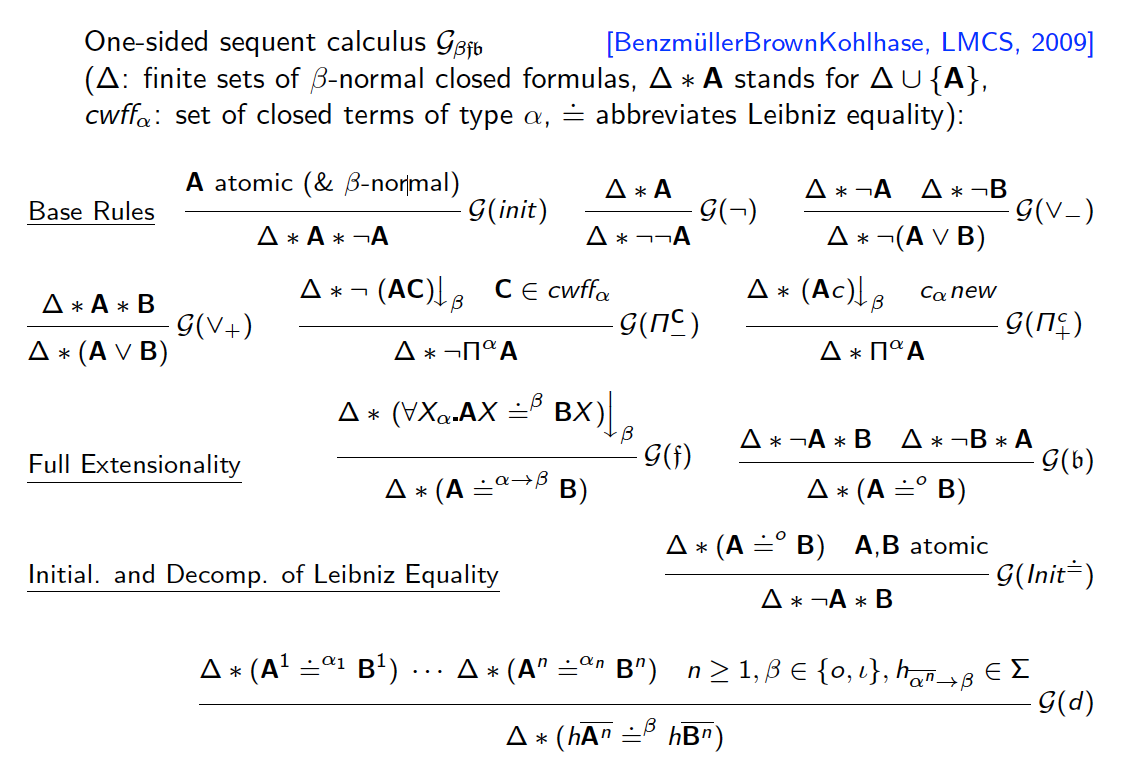
\includegraphics[width=12cm]{./Images/Varia/HOLCutFreeSequentCalculus.png}
% % \end{changemargin}
% % \end{frame}



% \begin{transitionframe}{./Images/Transitions/GodComputerC}{black}
% \textbf{
% \quad Automated and Interactive Theorem Provers for \textcolor{Blue}{HOL}
% }
% \end{transitionframe}






% \begin{frame}{Automated Theorem Provers and Model Finders for HOL}
% 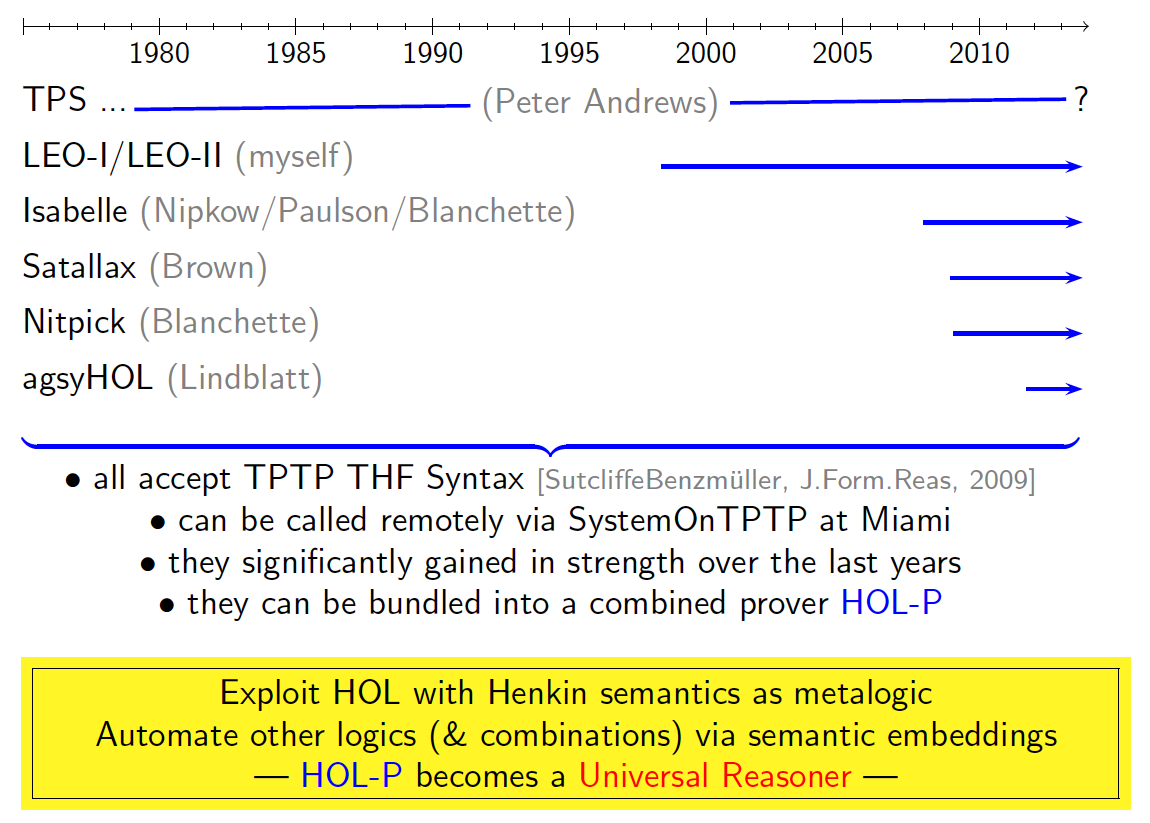
\includegraphics[width=1.05\textwidth]{./Images/HOLProversGrab}
% \end{frame}





% % \begin{frame}
% %   \frametitle{EU Project THFTPTP: An Infrastructure for HOL-ATP}
% % \begin{block}{Results of the EU Project THFTPTP (2006/2007)}
% % \begin{itemize}
% % \item Collaboration with Geoff Sutcliffe, Chad Brown and others
% % \item Results
% % \begin{itemize}
% % \item THF0 syntax for HOL
% % \item Online access to provers
% % \item Library with example problems (e.g. entire TPS library) and results
% % \item Ontology and syntax for proof results
% % \item International CASC competition for HOL-ATP
% % \item Various tools 
% % \end{itemize}
% % \end{itemize}
% % \end{block}
% % \vfill
% % Improved availability and robustness of HOL-ATPs: \\
% % \qquad TPS, LEO-II, Isabelle, Satallax, Refute, Nitpick, agsyHOL, coqATP \\
% % \qquad Online access: \url{http://www.tptp.org/cgi-bin/SystemOnTPTP}
% % \vfill
% % \, \hfill   {\tiny \chriscite{SutcliffeBenzm{\"u}ller, J.~Formalized Reasoning, 2010}}\\
% % \, \hfill   {\tiny \chriscite{Benzm{\"u}llerRabeSutcliffe, IJCAR, 2008}}
% % \end{frame}



% % \begin{frame}{Proof Automation and Consistency Checking} 
% % \colorbox{gray}{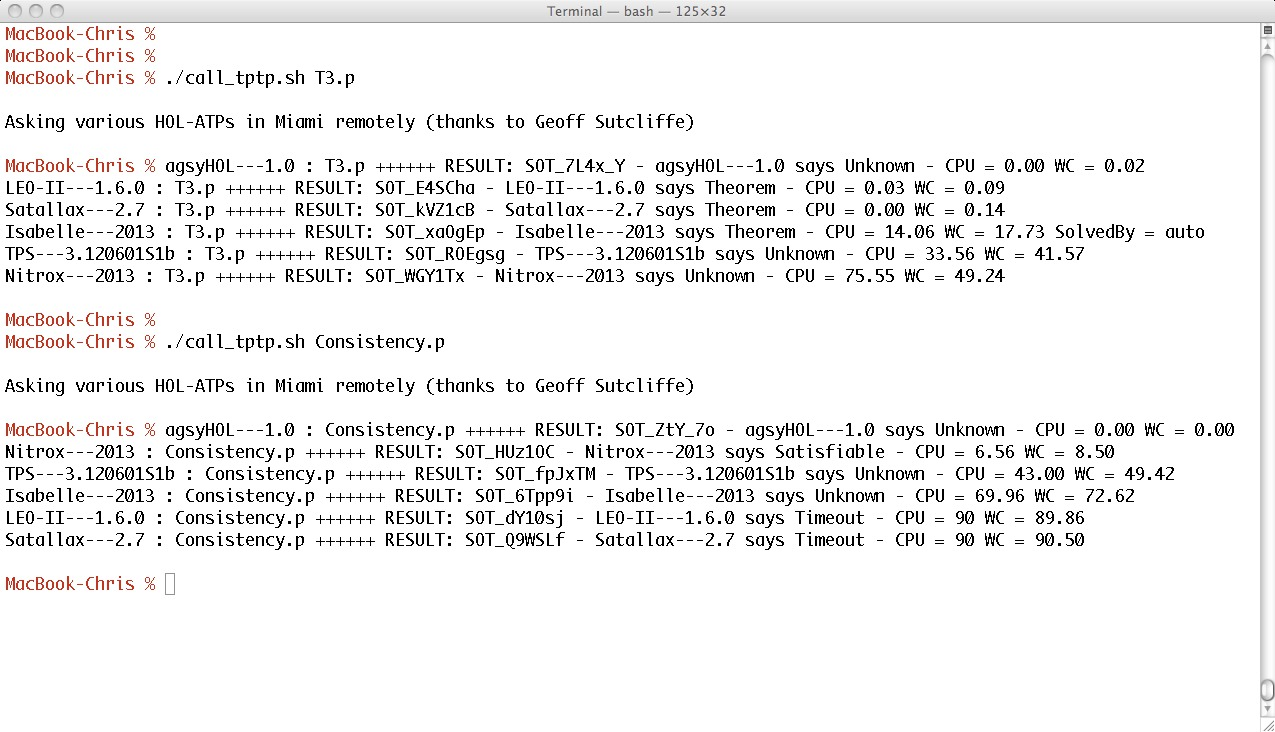
\includegraphics[width=\textwidth]{./Images/Demos/DemoGrap}} 
% % Provers can be called remotely in Miami --- no local installation needed!
% % \vfill
% % Download our experiments from \url{https://github.com/FormalTheology/GoedelGod/tree/master/Formalizations/THF}
% % \end{frame}


% \begin{frame}{Proof Automation with LEO-II} 
% %\colorbox{gray}{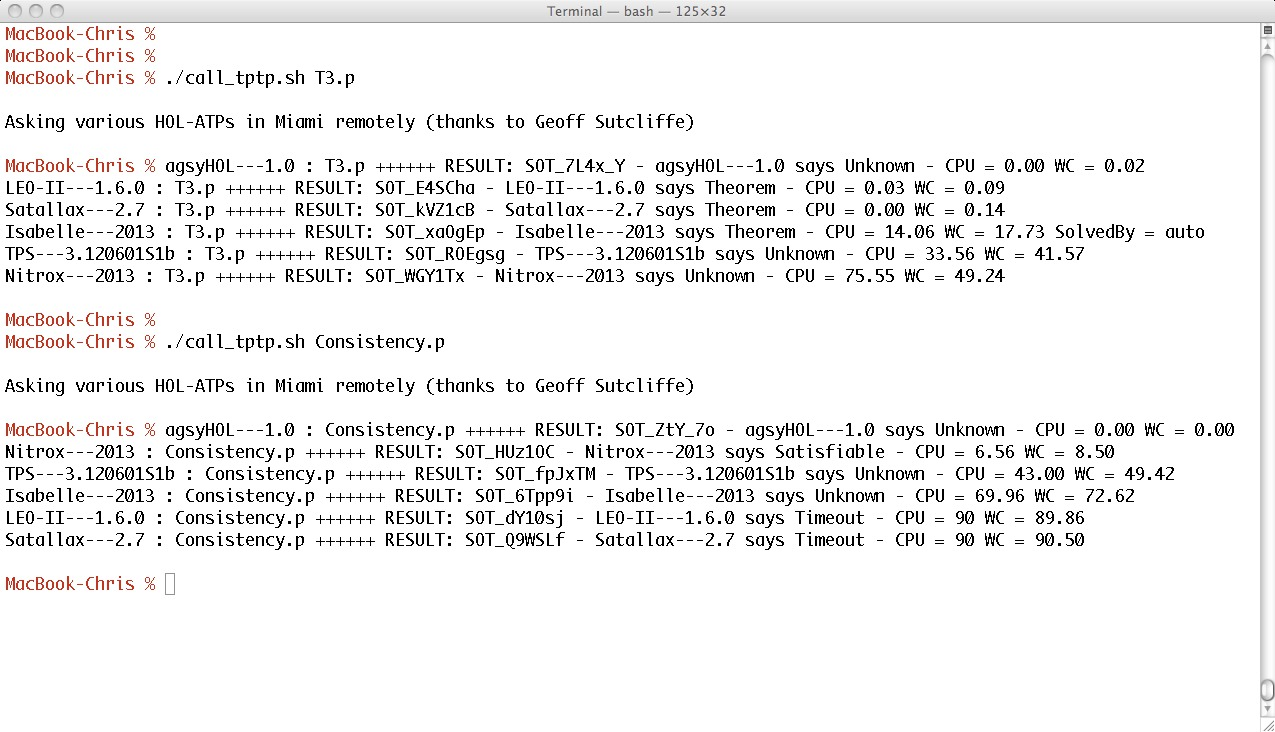
\includegraphics[width=\textwidth]{./Images/Demos/DemoGrap}} 
% %\colorbox{gray}{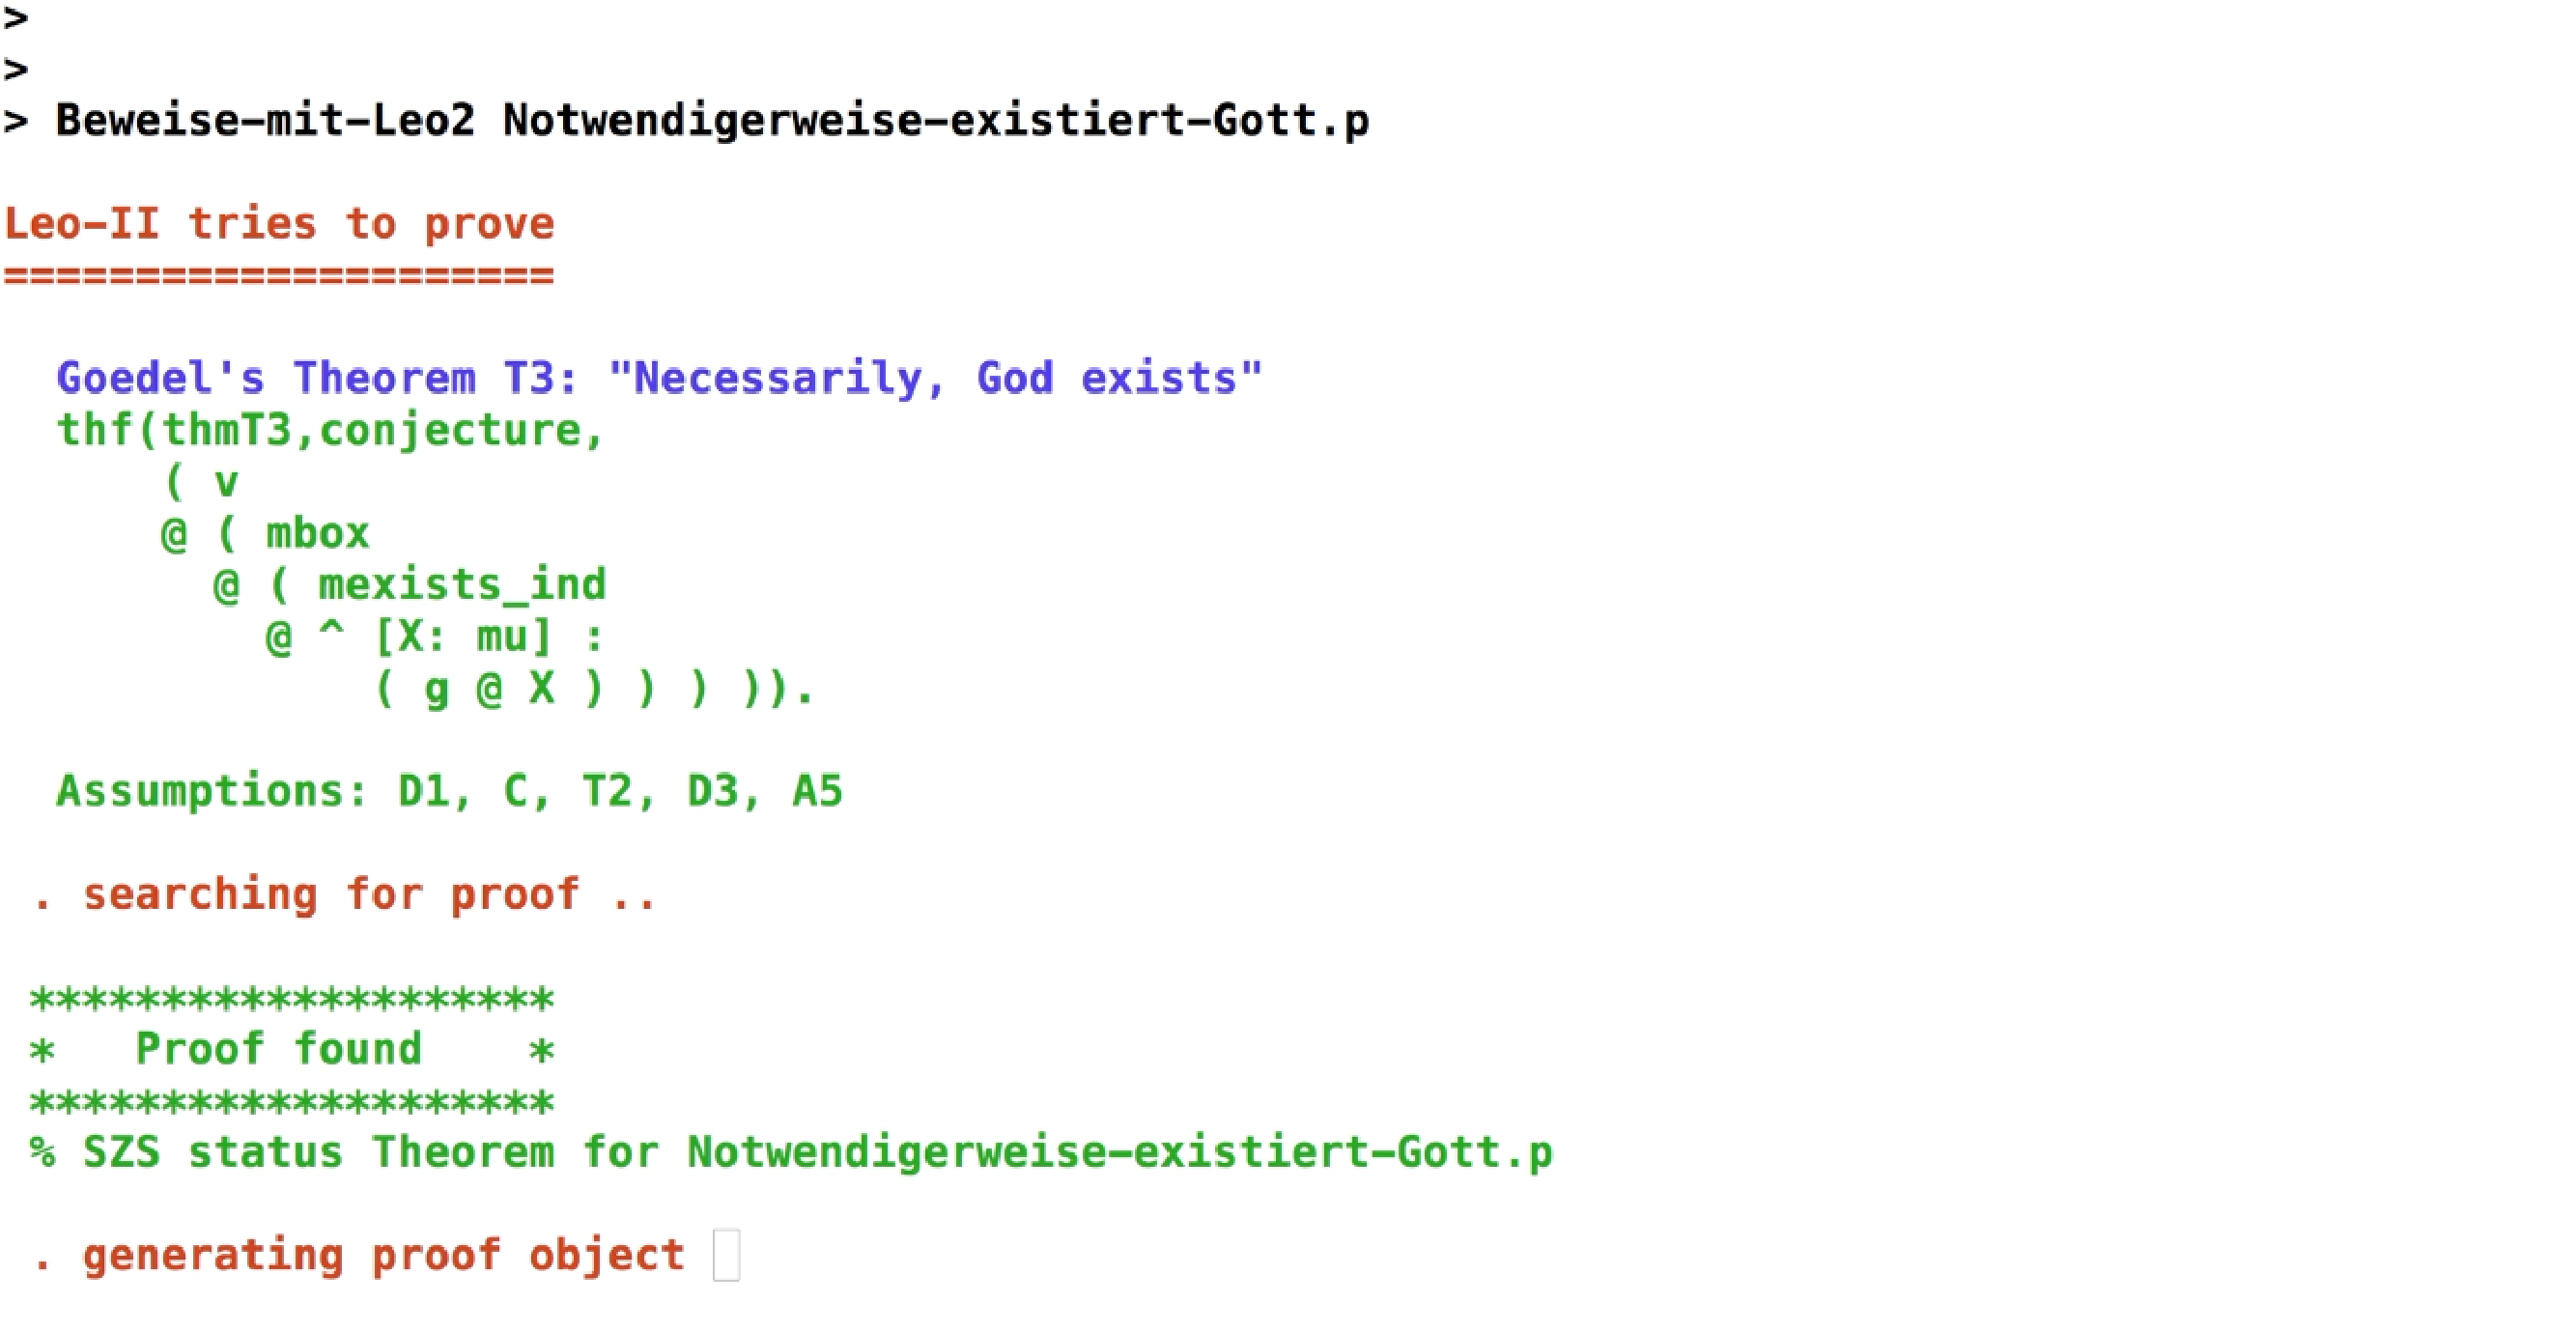
\includegraphics[width=\textwidth]{./Images/Movie1.pdf}} 
% \movie[height=6cm,width=10cm,loop]{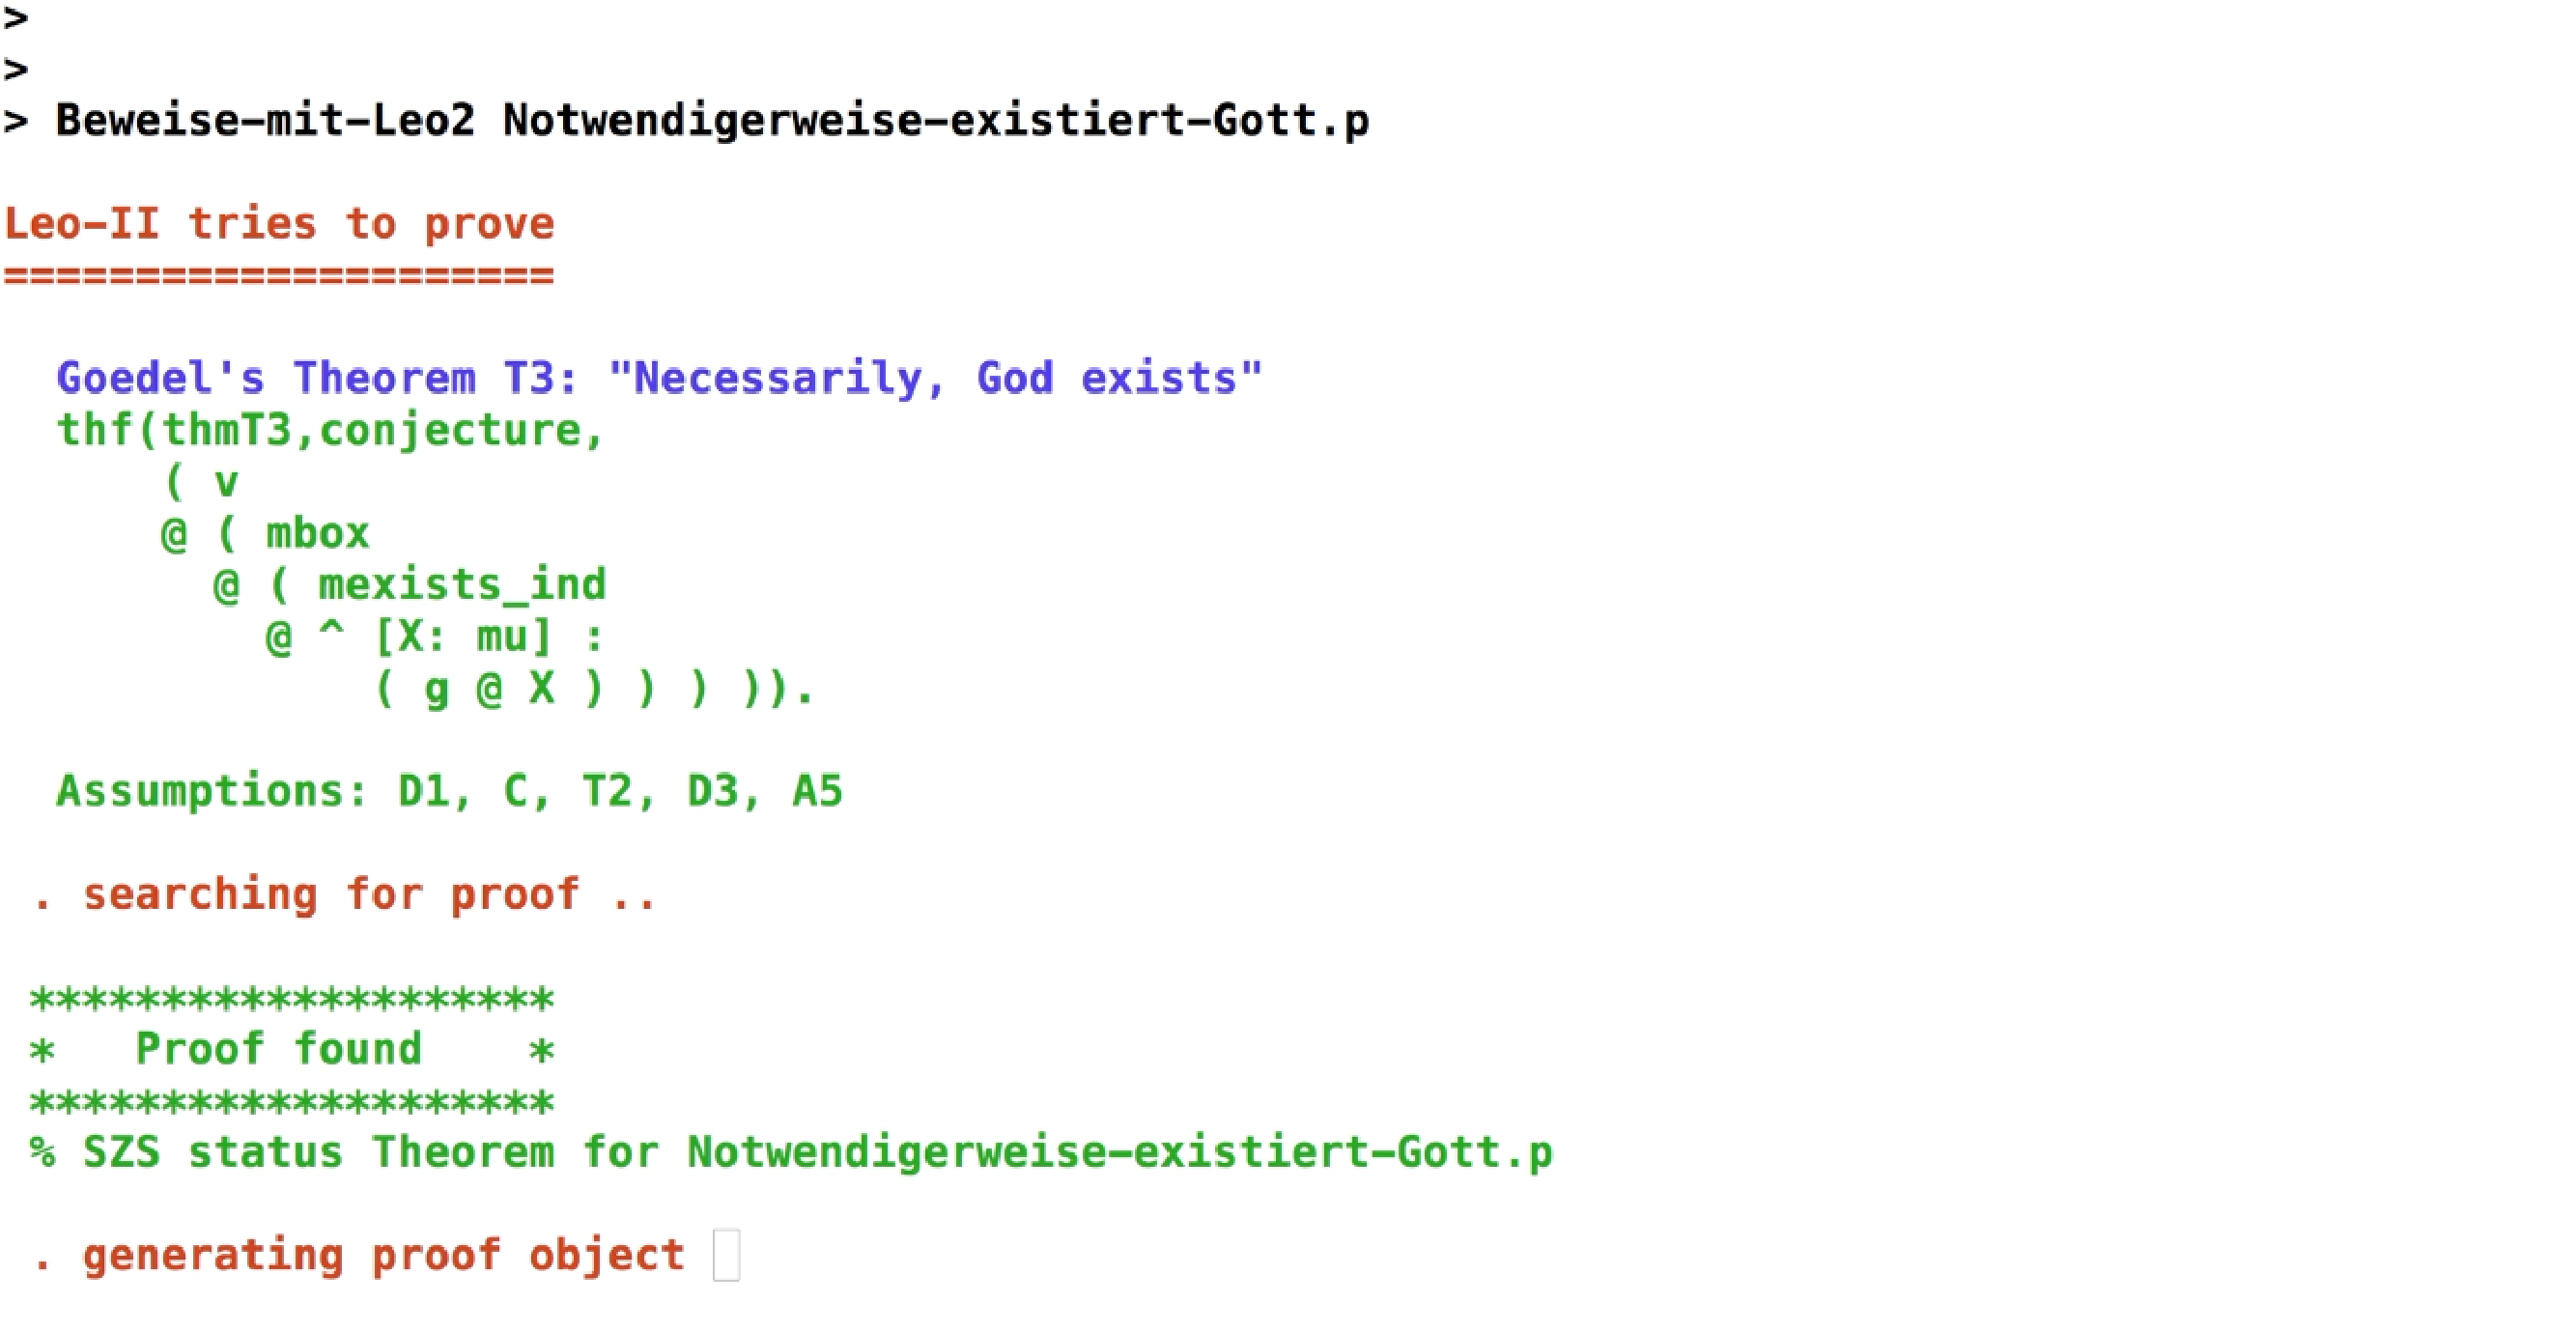
\includegraphics[height=6cm,width=10cm]{./Images/Movie1.pdf}}{./Images/Movie1.mov}
% \vfill 
% Provers can be called remotely in Miami --- no local installation needed!
% \vfill
% Download our experiments from \\
% {\footnotesize \url{https://github.com/FormalTheology/GoedelGod/tree/master/Formalizations/THF}}
% \end{frame}





% % \begin{transitionframe}{./Images/Transitions/PaganReligions(CC-BY-SA)}{white} \Large \centering
% % \quad Automation and Verification in \textsc{Isabelle/HOL} \\
% % \quad Interactive Verification in \textsc{Coq} \\[2em]
% % \end{transitionframe}


% \begin{frame}{G\"odel's God in Isabelle/HOL} \centering
% \vskip1em
% \begin{changemargin}{-0.5cm}{-.5cm}
% \colorbox{gray}{
% \movie[height=7cm,width=10.5cm,start=49s,duration=40s,loop]{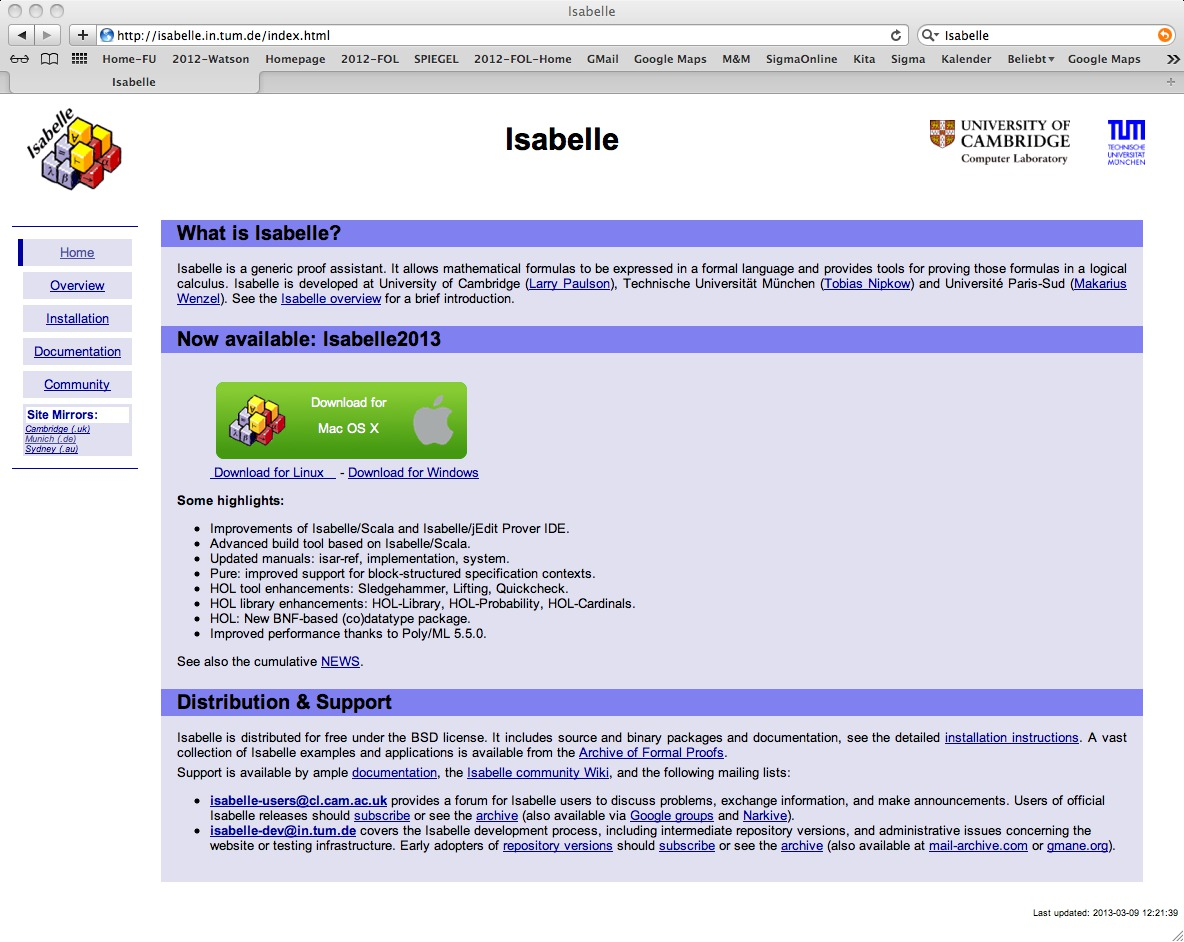
\includegraphics[height=7cm,width=10.5cm]{./Images/IsabelleGrab}}{./Images/Movie2.mov}
% %\includemovie[autopause,autoplay,autoresume,poster=/Users/cbenzmueller/chris/trunk/tex/talks/2015-TV/Movie1.pdf]{8cm}{4cm}{/Users/cbenzmueller/chris/trunk/tex/talks/2015-TV/Movie1.mov}
% }
% %colorbox{gray}{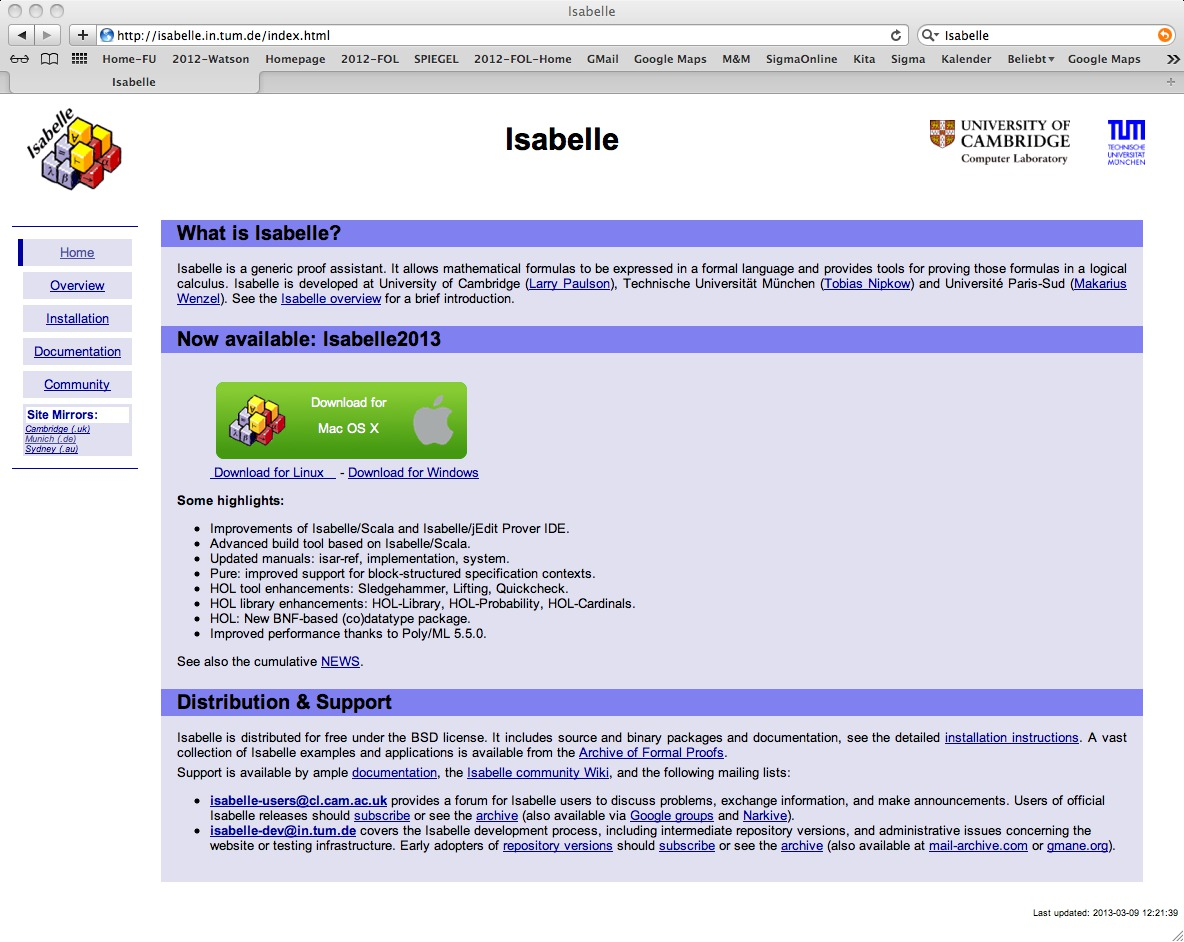
\includegraphics[width=\textwidth]{./Images/IsabelleGrab}}
% \vskip.3em
% \noindent See verifiable Isabelle/HOL document (Archive of Formal Proofs) at: \url{http://afp.sourceforge.net/entries/GoedelGod.shtml} 
% \end{changemargin}
% \end{frame}

% % \begin{frame}{Interaction and Automation in Proof Assistant \textsc{Isabelle/HOL}} \large \centering
% % \colorbox{gray}{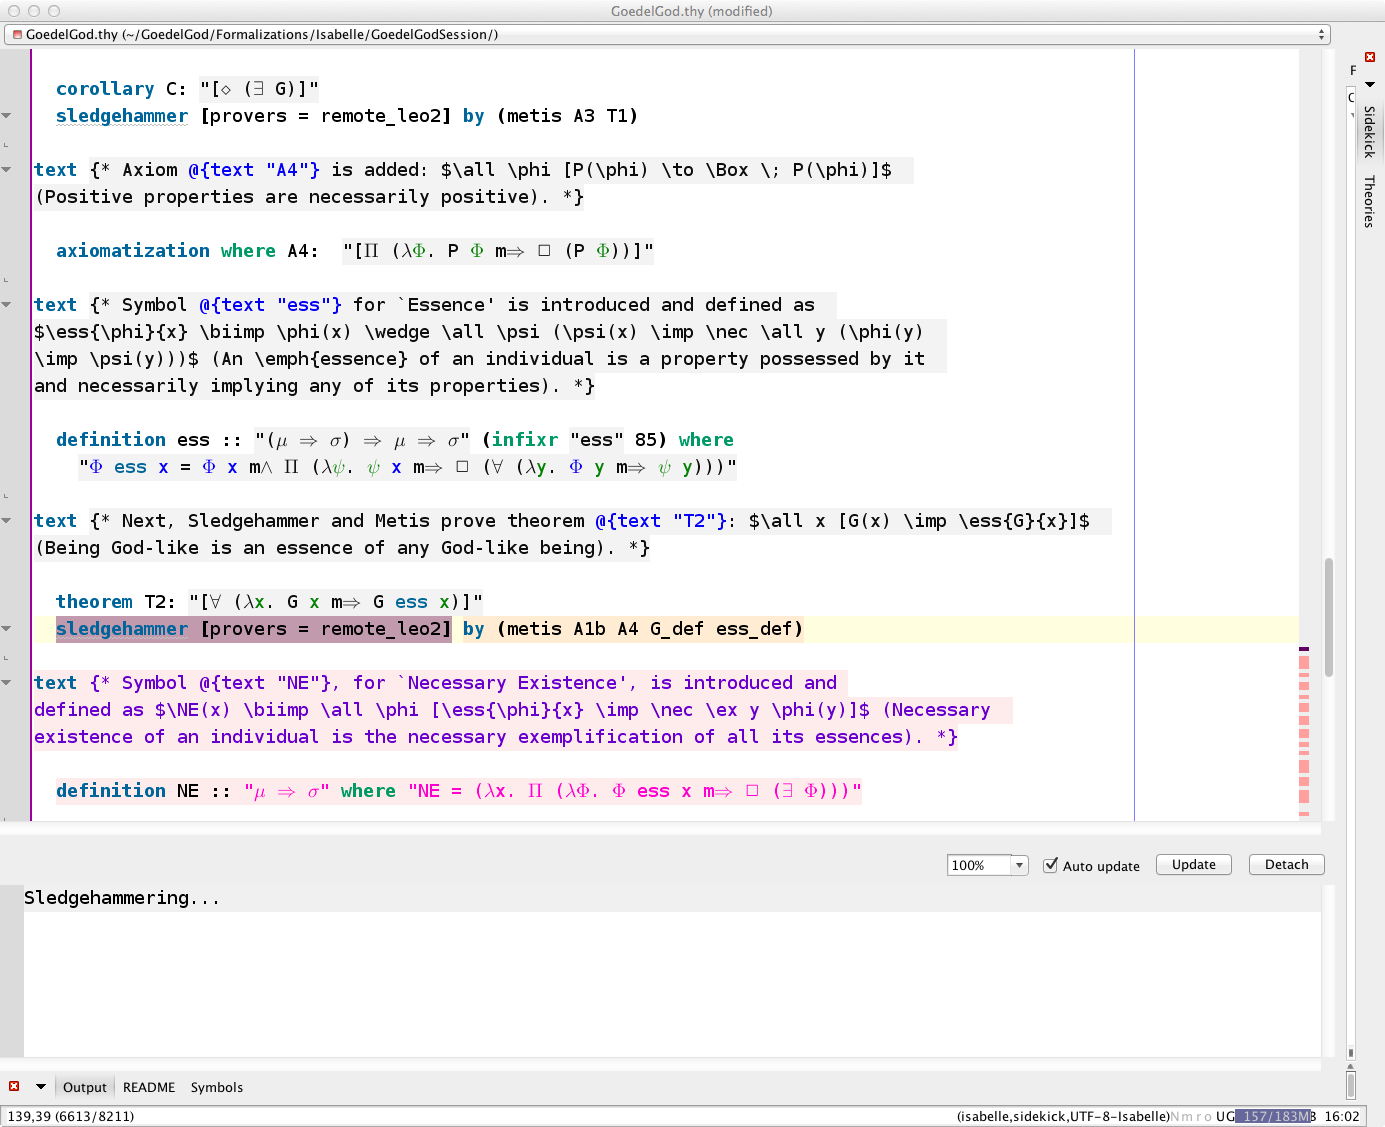
\includegraphics[width=.8\textwidth]{./Images/Demos/IsabelleDemoGrab}}\vfill
% % See verifiable Isabelle/HOL document (Archive of Formal Proofs) at: \url{http://afp.sourceforge.net/entries/GoedelGod.shtml}
% % \end{frame}




% % \begin{frame}{Automation \& Verification in Proof Assistant \textsc{Isabelle/HOL}} \large
% % Isabelle/HOL   (Cambridge University/TU Munich)
% % \begin{itemize}
% % \item HOL instance of the generic \textsc{Isabelle} proof assistant
% % \item User interaction and proof automation 
% % \item Automation is supported by \textsc{Sledgehammer} tool
% % \item Verification of the proofs in \textsc{Isabelle/HOL}'s small proof kernel
% % \end{itemize}
% % \vfill
% % What we did?
% % \begin{itemize}
% % \item Proof automation of G\"odel's proof script (Scott's version)
% % \item \textsc{Sledgehammer} makes calls to remote THF provers in Miami
% % \item These calls the suggest respective calls to the \textsc{Metis} prover
% % \item \textsc{Metis} proofs are verified in \textsc{Isabelle/HOL}'s proof kernel
% % \end{itemize}
% % \vfill
% % \begin{center}
% % --- see the handout (generated from the Isabelle source file) ---
% % \end{center}
% % \end{frame}

\begin{frame}{G\"odel's God in TPTP THF} \centering
\vskip1em
\colorbox{black!50}{
\movie[height=6.5cm,width=10cm,loop]{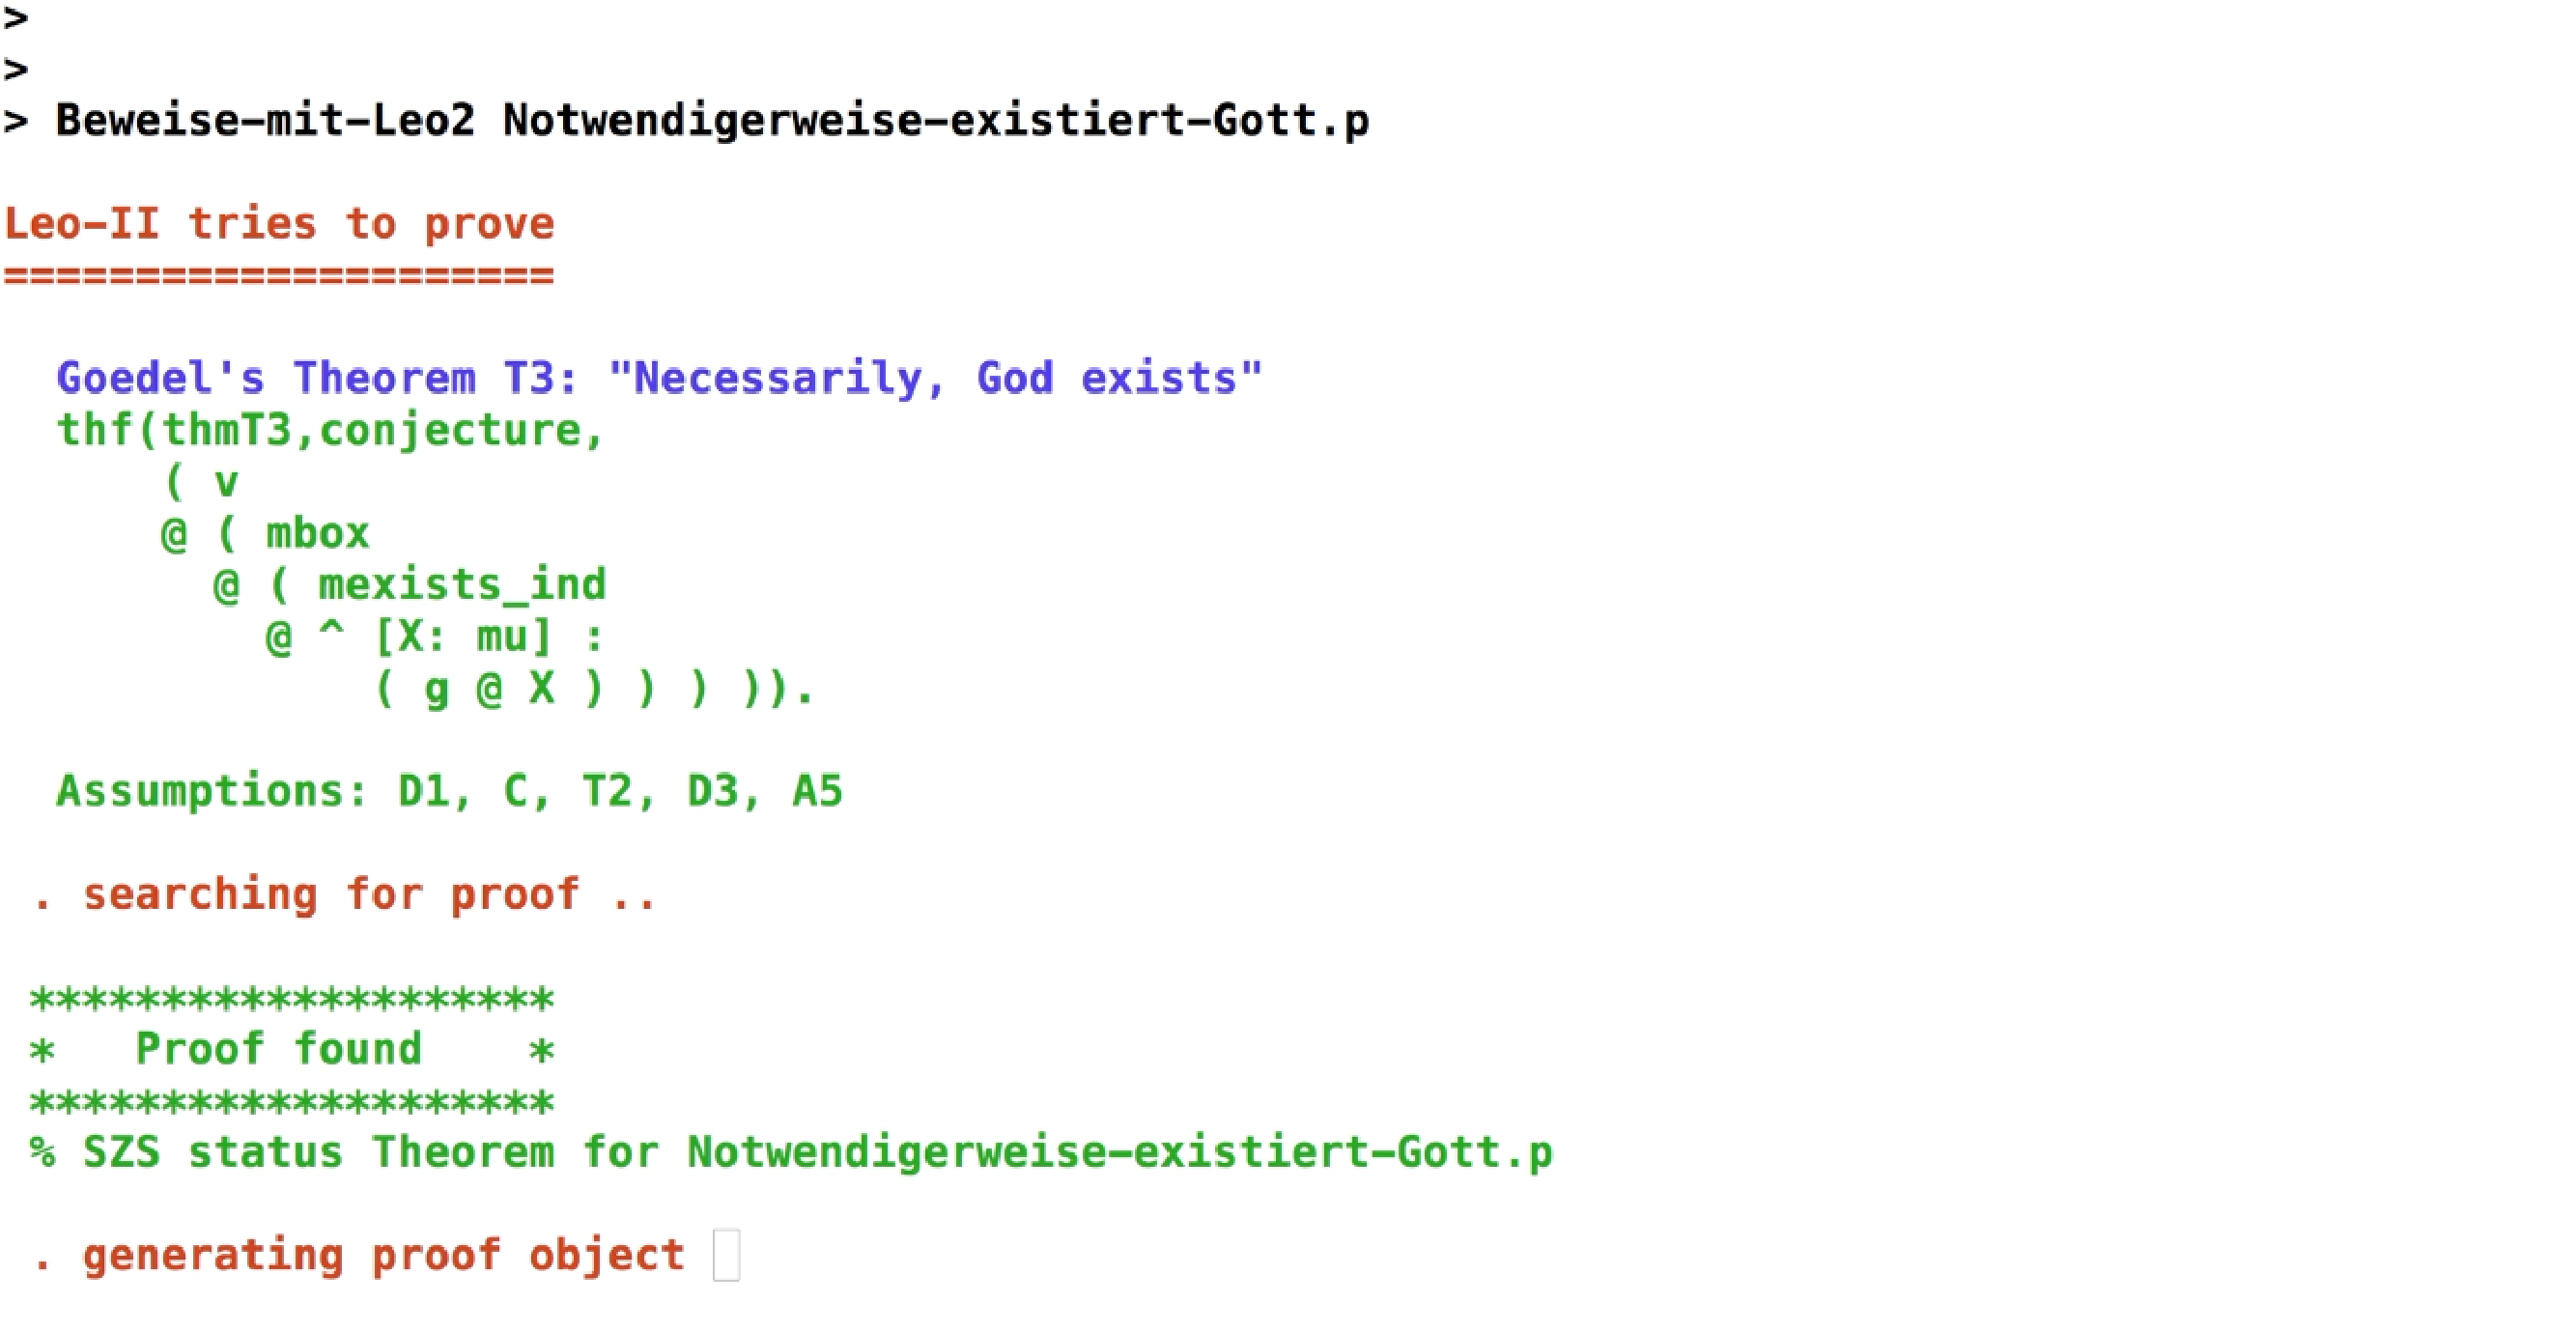
\includegraphics[height=6.5cm,width=10cm]{./Images/Movie1.pdf}}{./Images/Movie1.mov}
%\includemovie[autopause,autoplay,autoresume,poster=/Users/cbenzmueller/chris/trunk/tex/talks/2015-TV/Movie1.pdf]{8cm}{4cm}{/Users/cbenzmueller/chris/trunk/tex/talks/2015-TV/Movie1.mov}
}
\end{frame}

\begin{frame}{G\"odel's God in Isabelle/HOL} \centering
\vskip1em
%\begin{changemargin}{-0.5cm}{-.5cm}
\colorbox{gray}{
\movie[height=7cm,width=10.5cm,start=1s,stop=20s,loop]{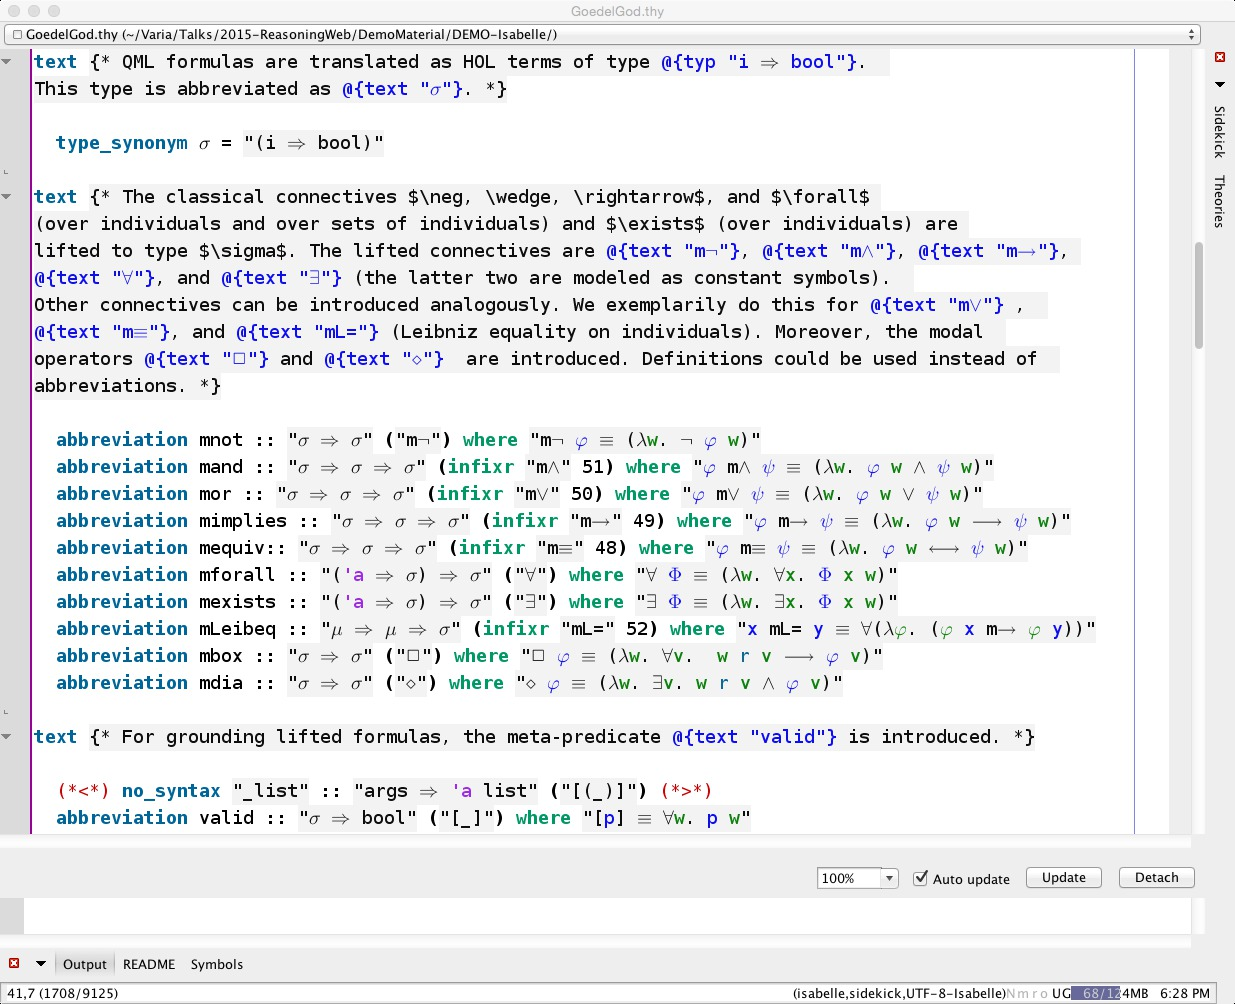
\includegraphics[height=7cm,width=10.5cm]{./Images/Varia/IsabelleGrab}}{./Images/Isabelle-T3.mov}
%\includemovie[autopause,autoplay,autoresume,poster=/Users/cbenzmueller/chris/trunk/tex/talks/2015-TV/Movie1.pdf]{8cm}{4cm}{/Users/cbenzmueller/chris/trunk/tex/talks/2015-TV/Movie1.mov}
}
%colorbox{gray}{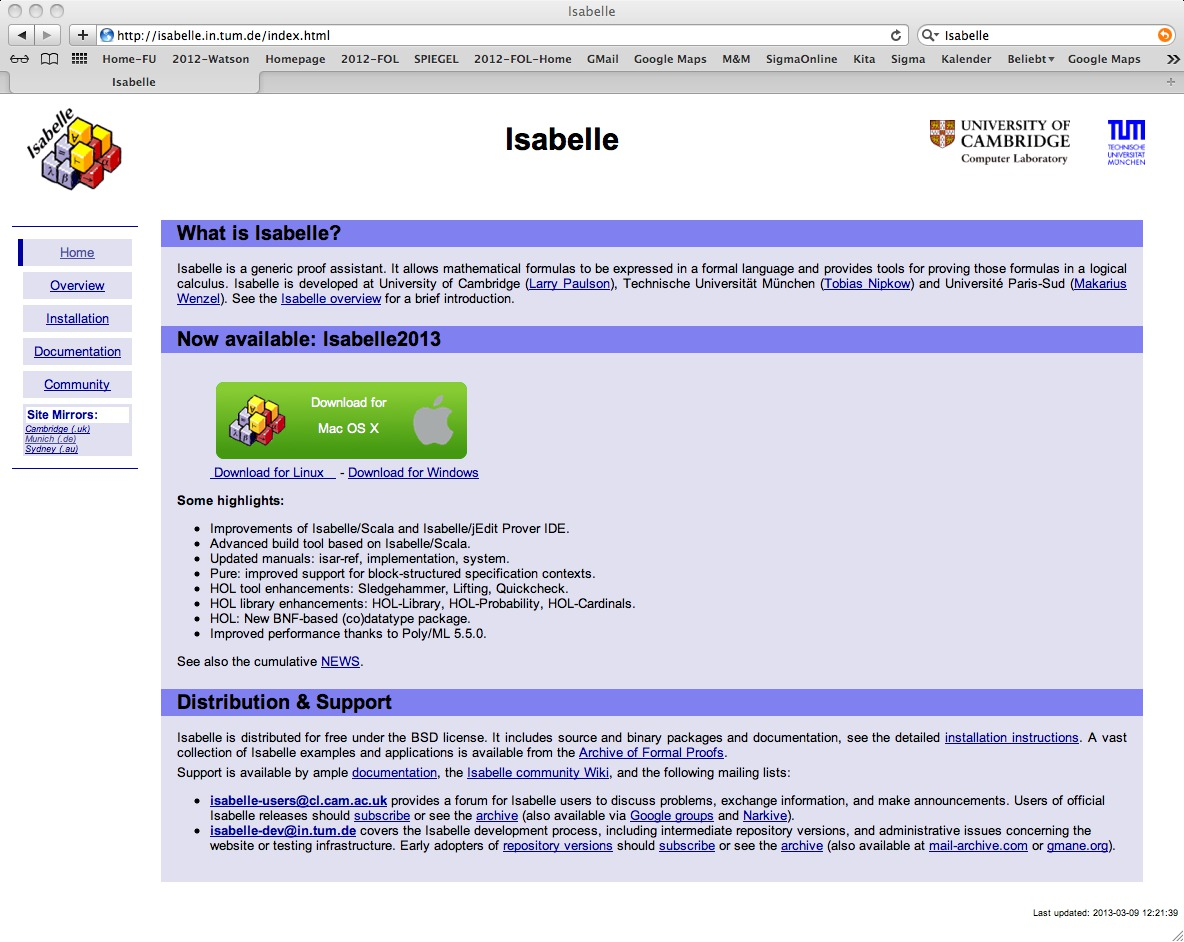
\includegraphics[width=\textwidth]{./Images/IsabelleGrab}}

\noindent See verifiable Isabelle/HOL document (Archive of Formal Proofs) at: \url{http://afp.sourceforge.net/entries/GoedelGod.shtml} 
%\end{changemargin}
\end{frame}


\begin{frame}{G\"odel's God in \textsc{Coq}} \large \centering
\colorbox{gray}{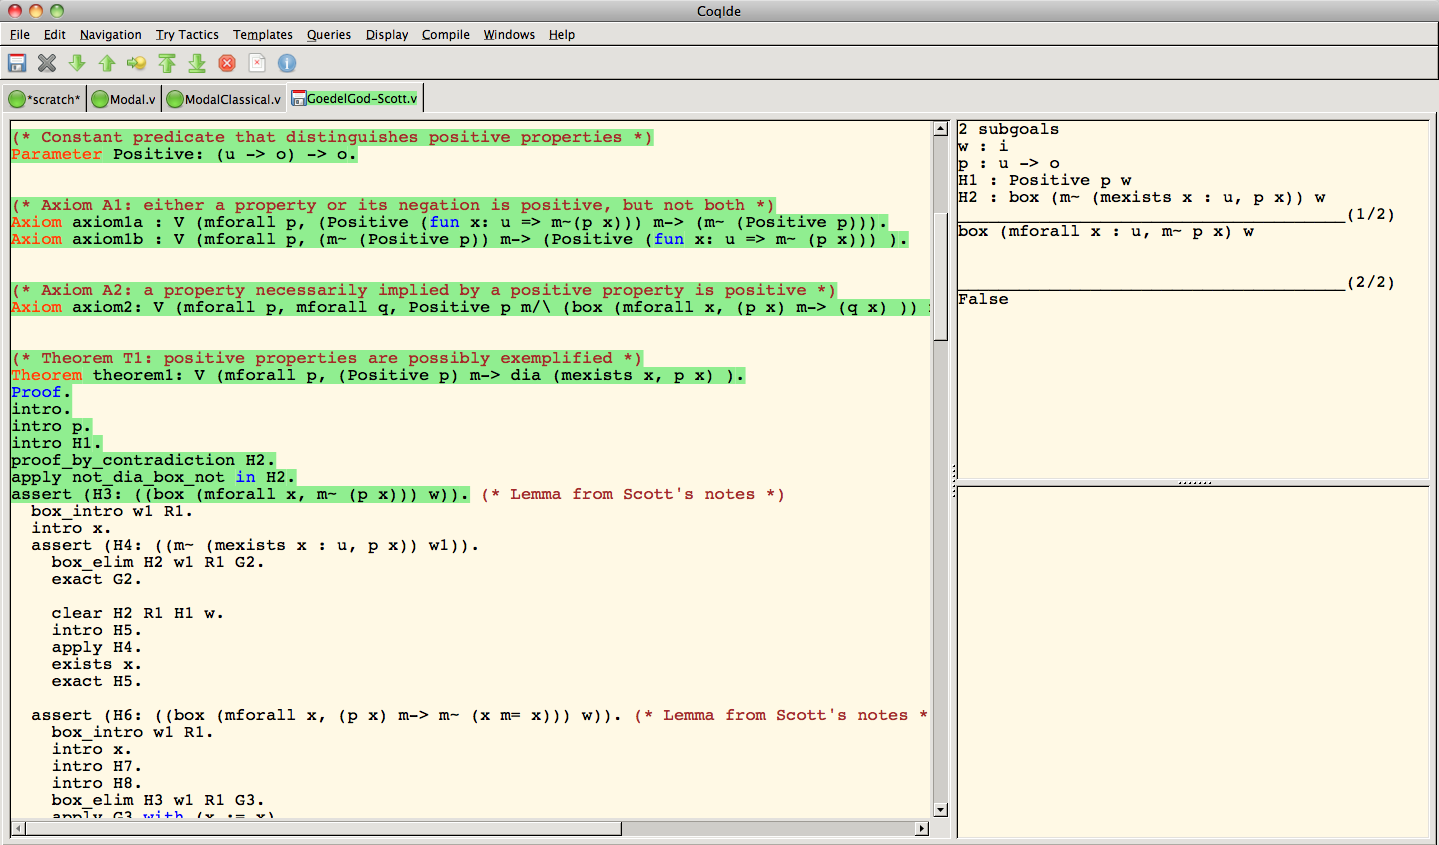
\includegraphics[width=1\textwidth]{./Images/Demos/CoqDemo.png}}
\vfill
See verifiable Coq document at: \\
{\footnotesize \url{https://github.com/FormalTheology/GoedelGod/tree/master/Formalizations/Coq}}
\end{frame}





% \begin{frame}{(Interim) Culmination of two decades of related own research}
% %Formal Methods \hfill \textcolor{gray}{(Diploma 1995)} \\[2cm]

% \begin{itemize} 
% \item Theory of classical higher-order logic (HOL) \hfill \textcolor{gray}{(since 1995)} 
% \item Automation of  HOL / own LEO  provers  \hfill \textcolor{gray}{(since 1998)} 

% \item Integration of interactive and automated theorem proving \, \hfill \textcolor{gray}{(since 1999)} 

% \item International TPTP infrastructure for HOL 
% \, \hfill \textcolor{gray}{(since 2006)} 

% \item HOL as a universal logic via semantic embeddings
%  \, \hfill \textcolor{gray}{(since 2008)} 

% \item \textbf{Application in Philosophy: Ontological Argument} 
% \, \hfill  \textcolor{gray}{(since 2013)} \\
%      (jww Bruno Woltzenlogel-Paleo)
% \end{itemize}
% \vskip1em
% \textcolor{gray}{\textit{\ldots\ success story (despite strong
%     criticism/opposition on the way!)\ \ldots}}

% \textcolor{gray}{\textit{\ldots\ huge media attention\ \ldots}}
% \vfill

% \end{frame}


% \begin{frame}{Results}
% \begin{changemargin}{-0.8cm}{-1.1cm}
% 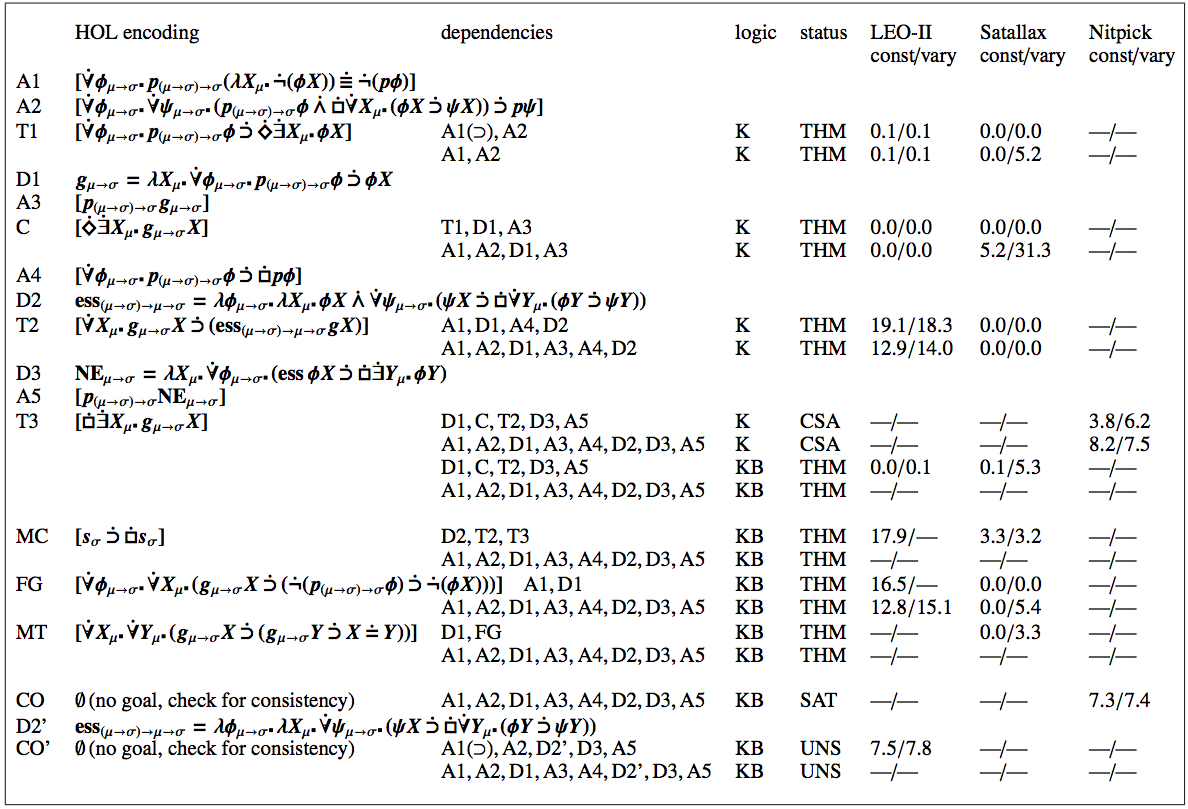
\includegraphics[width=12.4cm]{./Images/Results.png}
% \end{changemargin}
% \end{frame}


\begin{transitionframe}{./Images/Transitions/NietzscheGod3}{black}
\textbf{Findings from our study \\ \chriscite{Benzm\"ullerWoltzenlogelPaleo, ECAI, 2014}}
\end{transitionframe}


\usebackgroundtemplate{
  \vbox to \paperheight{\vfil\hbox to \paperwidth{\hfil
      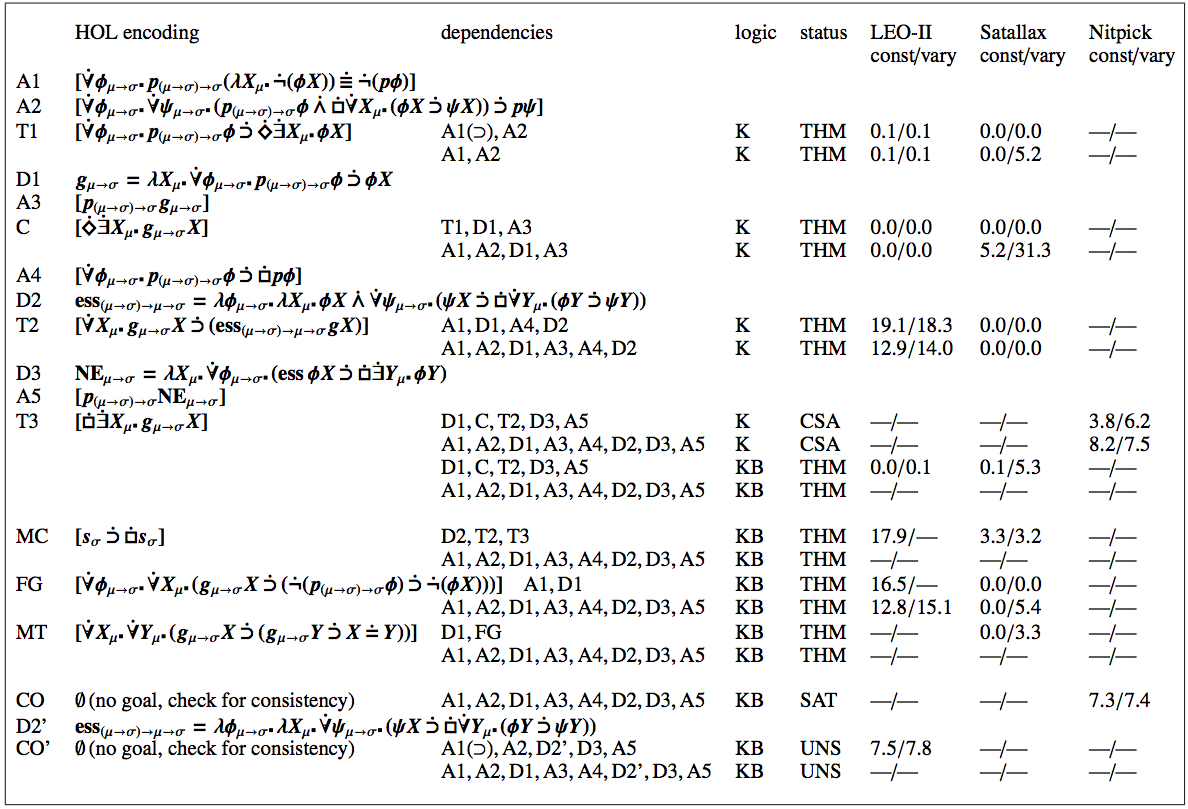
\includegraphics[width=11.5cm]{./Images/Results.png} 
      \hfil}\vfil}
}
%\usebackgroundtemplate{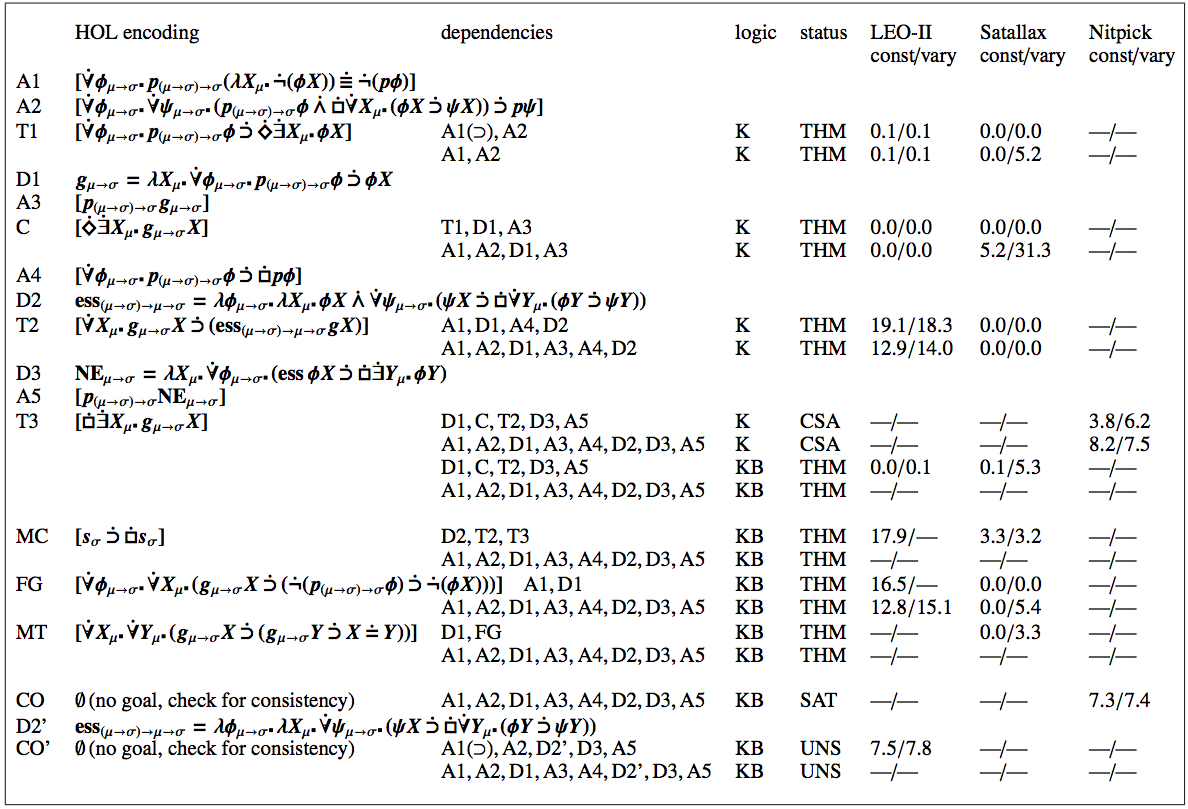
\includegraphics[width=\paperwidth]{./Images/Results.png}}
%\pgfsetlinewidth{10\pgflinewidth} 
%\pgfsetlinecolor{Blue} 

\begin{frame}{Main Findings \chriscite{Benzm\"ullerWoltzenlogelPaleo, ECAI, 2014}}

\end{frame}

\begin{frame}{Main Findings \chriscite{Benzm\"ullerWoltzenlogelPaleo, ECAI, 2014}}
\begin{changemargin}{-.2cm}{-.5cm}
\begin{pgfpicture}{0cm}{0cm}{11cm}{11cm}
\pgfsetlinewidth{5\pgflinewidth} 
\pgfsetendarrow{\pgfarrowto}
%\pgfsetstartarrow{\pgfarrowto}
%\pgfnodecircle{Node1}[stroke]{\pgfxy(0,9.5)}{0.25cm}
\pgfnodebox{Node1}[stroke]{\pgfxy(5.6,8)}{\phantom{Bla}}{5.6cm}{2.1cm}
\end{pgfpicture}
\end{changemargin}
\end{frame}

\setbeamercovered{invisible}

\begin{frame}{Main Findings \chriscite{Benzm\"ullerWoltzenlogelPaleo, ECAI, 2014}}
\begin{changemargin}{-.2cm}{-.5cm}
\begin{pgfpicture}{0cm}{0cm}{11cm}{11cm}
\pgfsetlinewidth{5\pgflinewidth} 
\pgfsetendarrow{\pgfarrowto}
%\pgfsetstartarrow{\pgfarrowto}
%\pgfnodecircle{Node1}[stroke]{\pgfxy(0,9.5)}{0.25cm}
\pgfnodebox{Node1}[stroke]{\pgfxy(5.6,9.45)}{\phantom{Bla}}{5.6cm}{.2cm}
\pgfnodebox{Node2}[virtual]{\pgfxy(7,5)}{
\framecolorbox[8.5cm][s]{Green}{green!20}{
\begin{minipage}{8cm}\color{black} \bf
%\vskip1em
\underline{Automating Scott's proof script} \\[1em]
{T1: "Positive properties are possibly exemplified"}
proved by LEO-II and Satallax 
\begin{itemize}
\item  in logic: K 
\item  from assumptions:
  \begin{itemize} 
  \item A1 and A2
  \item \onslide<1->{\color{black} A1($\supset$) and A2}
  \end{itemize}
\item notion of quantification
  \begin{itemize} 
  \item possibilist quantifiers (constant dom.)
  \item actualist quantifiers for individuals (varying dom.)
  \end{itemize}
\end{itemize}
\vspace*{1em}
\end{minipage}
}}{2pt}{2pt}
\pgfnodeconncurve{Node1}{Node2}{180}{180}{1cm}{2cm}
\end{pgfpicture}
\end{changemargin}
\end{frame}

\begin{frame}{Main Findings \chriscite{Benzm\"ullerWoltzenlogelPaleo, ECAI, 2014}}
\begin{changemargin}{-.2cm}{-.5cm}
\begin{pgfpicture}{0cm}{0cm}{11cm}{11cm}
\pgfsetlinewidth{5\pgflinewidth} 
\pgfsetendarrow{\pgfarrowto}
%\pgfsetstartarrow{\pgfarrowto}
%\pgfnodecircle{Node1}[stroke]{\pgfxy(0,9.5)}{0.25cm}
\pgfnodebox{Node1}[stroke]{\pgfxy(5.6,8.5)}{\phantom{Bla}}{5.6cm}{.2cm}
\pgfnodebox{Node2}[virtual]{\pgfxy(7,5)}{
\framecolorbox[8.5cm][s]{Green}{green!20}{
\begin{minipage}{8cm}\color{black} \bf
%\vskip1em
\underline{Automating Scott's proof script} \\[1em]
C: "Possibly, God exists'' \\
proved by LEO-II and Satallax 
\begin{itemize}
\item  in logic: K 
\item  from assumptions:
  \begin{itemize} 
  \item T1, D1, A3
%  \item A1, A2, D1, A3
  \end{itemize}
\item for domain conditions: 
  \begin{itemize} 
  \item possibilist quantifiers (constant dom.)
  \item actualist quantifiers for individuals (varying dom.)
  \end{itemize}
\end{itemize}
\vspace*{1em}
\end{minipage}
}}{2pt}{2pt}
\pgfnodeconncurve{Node1}{Node2}{180}{180}{1cm}{2cm}
\end{pgfpicture}
\end{changemargin}
\end{frame}


\begin{frame}{Main Findings \chriscite{Benzm\"ullerWoltzenlogelPaleo, ECAI, 2014}}
\begin{changemargin}{-.2cm}{-.5cm}
\begin{pgfpicture}{0cm}{0cm}{11cm}{11cm}
\pgfsetlinewidth{5\pgflinewidth} 
\pgfsetendarrow{\pgfarrowto}
%\pgfsetstartarrow{\pgfarrowto}
%\pgfnodecircle{Node1}[stroke]{\pgfxy(0,9.5)}{0.25cm}
\pgfnodebox{Node1}[stroke]{\pgfxy(5.6,7.6)}{\phantom{Bla}}{5.6cm}{.2cm}
\pgfnodebox{Node2}[virtual]{\pgfxy(7,5)}{
\framecolorbox[8.5cm][s]{Green}{green!20}{
\begin{minipage}{8cm}\color{black} \bf
%\vskip1em
\underline{Automating Scott's proof script} \\[1em]
T2: "Being God-like is an ess. of any God-like being'' \\
proved by LEO-II and Satallax 
\begin{itemize}
\item  in logic: K 
\item  from assumptions:
  \begin{itemize} 
  \item A1, D1, A4, D2
%  \item A1, A2, D1, A3, A4, D2
  \end{itemize}
\item for domain conditions: 
  \begin{itemize} 
  \item possibilist quantifiers (constant dom.)
  \item actualist quantifiers for individuals (varying dom.)
  \end{itemize}
\end{itemize}
\vspace*{1em}
\end{minipage}
}}{2pt}{2pt}
\pgfnodeconncurve{Node1}{Node2}{180}{180}{1cm}{2cm}
\end{pgfpicture}
\end{changemargin}
\end{frame}



\begin{frame}{Main Findings \chriscite{Benzm\"ullerWoltzenlogelPaleo, ECAI, 2014}}
\begin{changemargin}{-.2cm}{-.5cm}
\begin{pgfpicture}{0cm}{0cm}{11cm}{11cm}
\pgfsetlinewidth{5\pgflinewidth} 
\pgfsetendarrow{\pgfarrowto}
%\pgfsetstartarrow{\pgfarrowto}
%\pgfnodecircle{Node1}[stroke]{\pgfxy(0,9.5)}{0.25cm}
\pgfnodebox{Node1}[stroke]{\pgfxy(5.6,6.6)}{\phantom{Bla}}{5.6cm}{.2cm}
\pgfnodebox{Node2}[virtual]{\pgfxy(7,5)}{
\framecolorbox[8.5cm][s]{Green}{green!20}{
\begin{minipage}{8cm}\color{black} \bf
%\vskip1em
\underline{Automating Scott's proof script} \\[1em]
T3: "Necessarily, God exists'' \\
proved by LEO-II and Satallax 
\begin{itemize}
\item  in logic: {\color{Blue} KB}
\item  from assumptions:
  \begin{itemize} 
  \item D1, C, T2, D3, A5
%  \item A1, A2, D1, A3, A4, D2
  \end{itemize}
\item for domain conditions: 
   \begin{itemize} 
  \item possibilist quantifiers (constant dom.)
  \item actualist quantifiers for individuals (varying dom.)
  \end{itemize}
\end{itemize}
For logic {\color{red} K} we got a {\color{red} countermodel} by Nitpick
\vspace*{1em}
\end{minipage}
}}{2pt}{2pt}
\pgfnodeconncurve{Node1}{Node2}{180}{180}{1cm}{2cm}
\end{pgfpicture}
\end{changemargin}
\end{frame}




\begin{frame}{Main Findings \chriscite{Benzm\"ullerWoltzenlogelPaleo, ECAI, 2014}}
\begin{changemargin}{-.2cm}{-.5cm}
\begin{pgfpicture}{0cm}{0cm}{11cm}{11cm}
\pgfsetlinewidth{5\pgflinewidth} 
\pgfsetendarrow{\pgfarrowto}
%\pgfsetstartarrow{\pgfarrowto}
%\pgfnodecircle{Node1}[stroke]{\pgfxy(0,9.5)}{0.25cm}
\pgfnodebox{Node1}[stroke]{\pgfxy(5.6,8)}{\phantom{Bla}}{5.6cm}{2.1cm}
\pgfnodebox{Node2}[virtual]{\pgfxy(7,5)}{
\framecolorbox[8.5cm][s]{Green}{green!20}{
\begin{minipage}{8cm}\color{black} \bf
%\vskip1em
\underline{Automating Scott's proof script} \\[1em]
Summary
\begin{itemize}
\item  proof verified and automated 
\item  {\color{Blue} KB} is sufficient  (critisized logic {\color{red} S5 not needed!}) 
\item  {\color{Blue} possibilist and actualist
    quantifiers (individuals)}
\item  {\color{Blue} exact dependencies} determined experimentally
\item  ATPs have found {\color{Blue} alternative proofs} \\
  \quad e.g. self-identity $\lambda x (x = x)$ is not needed 
\end{itemize}
\vspace*{1em}
\end{minipage}
}}{2pt}{2pt}
\pgfnodeconncurve{Node1}{Node2}{180}{180}{1cm}{2cm}
\end{pgfpicture}
\end{changemargin}
\end{frame}




\begin{frame}{Main Findings \chriscite{Benzm\"ullerWoltzenlogelPaleo, ECAI, 2014}}
\begin{changemargin}{-.2cm}{-.5cm}
\begin{pgfpicture}{0cm}{0cm}{11cm}{11cm}
\pgfsetlinewidth{5\pgflinewidth} 
\pgfsetendarrow{\pgfarrowto}
%\pgfsetstartarrow{\pgfarrowto}
%\pgfnodecircle{Node1}[stroke]{\pgfxy(0,9.5)}{0.25cm}
\pgfnodebox{Node1}[stroke]{\pgfxy(5.6,3.7)}{\phantom{Bla}}{5.6cm}{.4cm}
\pgfnodebox{Node2}[virtual]{\pgfxy(7,8)}{
\framecolorbox[8.5cm][s]{Green}{red!20}{
\begin{minipage}{8cm}\color{black} \bf
%\vskip1em
\underline{Consistency check: G\"odel vs. Scott} \\
\begin{itemize}
\item Scott's assumptions are consistent; \\ shown by Nitpick
\item G\"odel's assumptions are \textcolor{red}{inconsistent}; \\ shown by LEO-II
  \textcolor{red}{(new philosophical result!)} 
\end{itemize}
\vspace*{1em}
\end{minipage}
}}{2pt}{2pt}
\pgfnodeconncurve{Node1}{Node2}{180}{180}{1cm}{2cm}
\end{pgfpicture}
\end{changemargin}
\end{frame}



% \begin{frame}{Main Findings \chriscitebuf{Benzm\"ullerWoltzenlogelPaleo, ECAI, 2014}}
% \begin{changemargin}{-.2cm}{-.5cm}
% \begin{pgfpicture}{0cm}{0cm}{11cm}{11cm}
% \pgfsetlinewidth{5\pgflinewidth} 
% \pgfsetendarrow{\pgfarrowto}
% %\pgfsetstartarrow{\pgfarrowto}
% %\pgfnodecircle{Node1}[stroke]{\pgfxy(0,9.5)}{0.25cm}
% \pgfnodebox{Node1}[stroke]{\pgfxy(5.6,3.7)}{\phantom{Bla}}{5.6cm}{.4cm}
% \pgfnodebox{Node2}[virtual]{\pgfxy(7,5)}{
% \framecolorbox[8.5cm][s]{red}{red!20}{
% \begin{minipage}{8cm} \bf
% \underline{Argument for inconsistency (from LEO-II's proof)} \\
% \begin{itemize}
% \item[L1] $\emptyset$ is essence of any entity: \hfill 
%   ${\allq x} [\ess{(\lambda{y}\lambda{w}\bot)}{x}]$ \\
% by D2 (ess)
% \item[L2] $\NE$ is not exemplified: \hfill $\mnot \exq x
%   \NE(x)$ \\
% by A1($\supset$), A2, A5, L1 and D2 (ess)
% \item[$\Rightarrow$] Inconsistency:\hfill $\bot$ \\
% by L2, T1 and A5 
% \end{itemize}
% \vspace*{1em}
% \end{minipage}
% }}{2pt}{2pt}
% \pgfnodeconncurve{Node1}{Node2}{180}{180}{1cm}{2cm}
% \end{pgfpicture}
% \end{changemargin}
% \end{frame}



\begin{frame}{Main Findings \chriscite{Benzm\"ullerWoltzenlogelPaleo, ECAI, 2014}}
\begin{changemargin}{-.2cm}{-.5cm}
\begin{pgfpicture}{0cm}{0cm}{11cm}{11cm}
\pgfsetlinewidth{5\pgflinewidth} 
\pgfsetendarrow{\pgfarrowto}
%\pgfsetstartarrow{\pgfarrowto}
%\pgfnodecircle{Node1}[stroke]{\pgfxy(0,9.5)}{0.25cm}
\pgfnodebox{Node1}[stroke]{\pgfxy(5.6,4.85)}{\phantom{Bla}}{5.6cm}{.4cm}
\pgfnodebox{Node2}[virtual]{\pgfxy(7,8)}{
\framecolorbox[8.5cm][s]{yellow}{yellow!20}{
\begin{minipage}{8cm}\color{black} \bf
%\vskip1em
\underline{Further Results} \\
\begin{itemize}
\item Monotheism holds
\item God is flawless
\end{itemize}
\vspace*{1em}
\end{minipage}
}}{2pt}{2pt}
\pgfnodeconncurve{Node1}{Node2}{180}{180}{1cm}{2cm}
\end{pgfpicture}
\end{changemargin}
\end{frame}



\begin{frame}{Main Findings \chriscite{Benzm\"ullerWoltzenlogelPaleo, ECAI, 2014}}
\begin{changemargin}{-.2cm}{-.5cm}
\begin{pgfpicture}{0cm}{0cm}{11cm}{11cm}
\pgfsetlinewidth{5\pgflinewidth} 
\pgfsetendarrow{\pgfarrowto}
%\pgfsetstartarrow{\pgfarrowto}
%\pgfnodecircle{Node1}[stroke]{\pgfxy(0,9.5)}{0.25cm}
\pgfnodebox{Node1}[stroke]{\pgfxy(5.6,5.55)}{\phantom{Bla}}{5.6cm}{.2cm}
\pgfnodebox{Node2}[virtual]{\pgfxy(7,8.5)}{
\framecolorbox[8.5cm][s]{yellow}{yellow!20}{
\begin{minipage}{8cm}\color{black} \bf
%\vskip.5em
\underline{Modal Collapse (Sobel)} 
\vskip.5em
{\large \[ {\color{red} \allq \varphi ( \varphi \mimpl \Box \varphi ) } \]}
\begin{itemize}
\item proved by LEO-II and Satallax
\item for possibilist and actualist quantification (ind.) \\[1em]
\end{itemize}
Main critique on G\"odel's ontological proof:
\begin{itemize}
\item there are no contingent truths
\item everything is determined / no free will
%\item why using modal logic in the first place?
\end{itemize}
\vspace*{.5em}
\end{minipage}
}}{2pt}{2pt}
\pgfnodeconncurve{Node1}{Node2}{180}{180}{1cm}{2cm}
\end{pgfpicture}
\end{changemargin}
\end{frame}


\begin{frame}{Main Findings \chriscite{Benzm\"ullerWoltzenlogelPaleo, ECAI, 2014}}
\begin{changemargin}{-.2cm}{-.5cm}
\begin{pgfpicture}{0cm}{0cm}{11cm}{11cm}
\pgfsetlinewidth{5\pgflinewidth} 
\pgfsetendarrow{\pgfarrowto}
%\pgfsetstartarrow{\pgfarrowto}
%\pgfnodecircle{Node1}[stroke]{\pgfxy(0,9.5)}{0.25cm}
\pgfnodebox{Node1}[stroke]{\pgfxy(9.7,6.4)}{\phantom{Bla}}{1.3cm}{3.4cm}
\pgfnodebox{Node2}[virtual]{\pgfxy(3,4.5)}{
\framecolorbox[6cm][s]{red}{Red!20}{
\begin{minipage}{5.7cm}\color{black} \bf
%\vskip.5em
\underline{Observation} 
\vskip.5em
\begin{itemize}
\item good  performance of ATPs
\item excellent match between argumentation granularity in papers and
  the reasoning strength of the ATPs
\end{itemize}
\vspace*{.5em}
\end{minipage}
}}{2pt}{2pt}
\pgfnodeconncurve{Node1}{Node2}{180}{90}{1cm}{2cm}
\end{pgfpicture}
\end{changemargin}
\end{frame}


\begin{frame}{Main Findings \chriscite{Benzm\"ullerWoltzenlogelPaleo, ECAI, 2014}}
\begin{changemargin}{-.2cm}{-.5cm}
\begin{pgfpicture}{0cm}{0cm}{11cm}{11cm}
\pgfsetlinewidth{5\pgflinewidth} 
\pgfsetendarrow{\pgfarrowto}
%\pgfsetstartarrow{\pgfarrowto}
%\pgfnodecircle{Node1}[stroke]{\pgfxy(0,9.5)}{0.25cm}
\pgfnodebox{Node1}[stroke]{\pgfxy(5.6,3.7)}{\phantom{Bla}}{5.6cm}{.4cm}
\pgfnodebox{Node2}[virtual]{\pgfxy(7,8)}{
\framecolorbox[8.5cm][s]{Green}{red!20}{
\begin{minipage}{8cm}\color{black} \bf
%\vskip1em
\underline{Consistency check: G\"odel vs. Scott} \\
\begin{itemize}
\item Scott's assumptions are consistent; \\ shown by Nitpick
\item G\"odel's assumptions are \textcolor{red}{inconsistent}; \\ shown by LEO-II
  \textcolor{red}{(new philosophical result!)} 
\end{itemize}
\vspace*{1em}
\end{minipage}
}}{2pt}{2pt}
\pgfnodeconncurve{Node1}{Node2}{180}{180}{1cm}{2cm}
\end{pgfpicture}
\end{changemargin}
\end{frame}




\usebackgroundtemplate{}


\begin{transitionframe}{./Images/Transitions/ComputerCross}{black}%$
  \centering
\textbf{Reconstruction of the Inconsistency of G\"odel's Axioms}
%\\ into Higher-Order Logic}
%\textbf{Embedding Higher-Order Modal Logic \\ into Higher-Order Logic}
\end{transitionframe}

\begin{frame}{Inconsistency (G\"odel): Proof by LEO-II in KB}
\begin{changemargin}{-.5cm}{-1cm}
\colorbox{gray!20}{
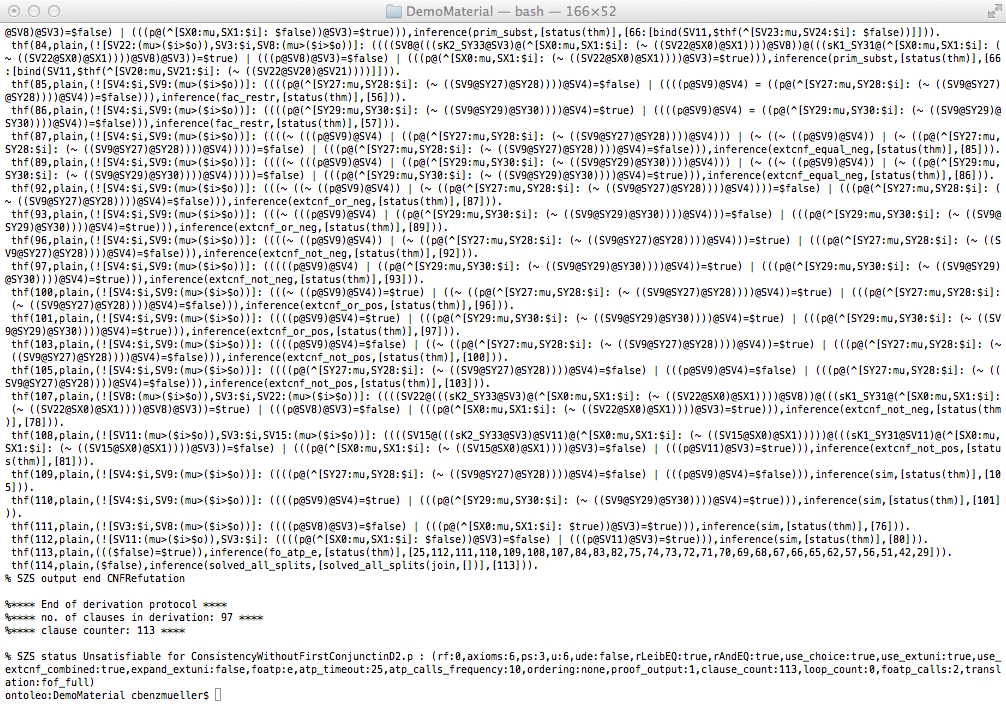
\includegraphics[width=11.5cm,height=8cm]{./DemoMaterial/LeoProof.png}
}
\end{changemargin}
\end{frame}



\begin{frame}{Inconsistency (G\"odel): Verification in Isabelle/HOL (KB)}
\begin{changemargin}{-.5cm}{-1cm}
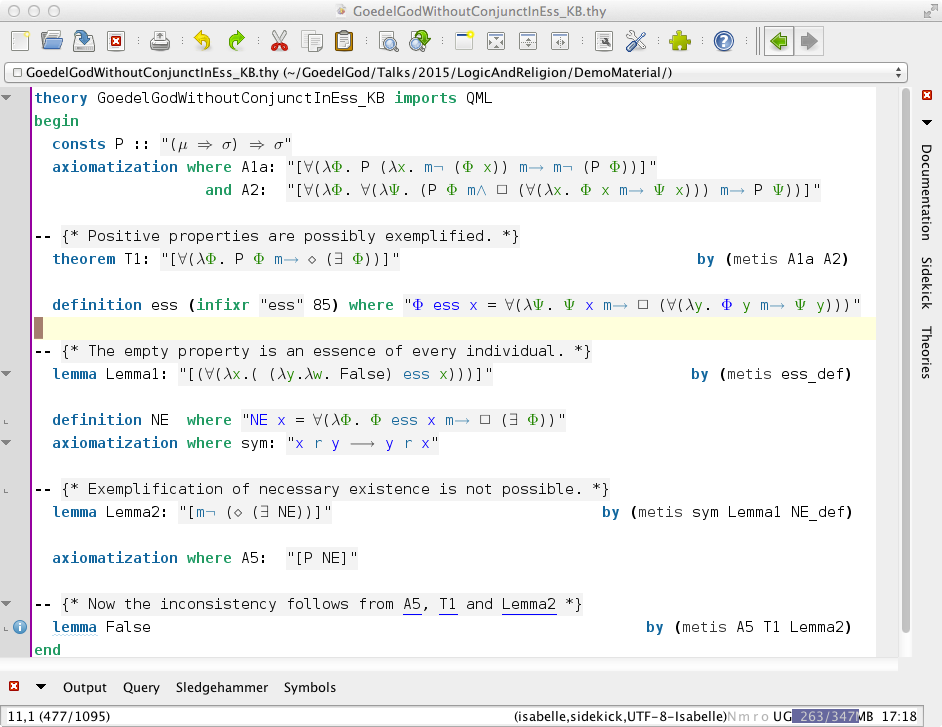
\includegraphics[width=12cm,height=8.5cm]{./DemoMaterial/GoedelGodWithoutConjunctInEss_KB.png}
\end{changemargin}
\end{frame}



\begin{frame}{Inconsistency (G\"odel): Reconstruction of Informal Argument (KB)}
\textcolor{gray}{(special thanks to Chad Brown for a fruitful discussion)} \\[1em]
\begin{flushright}
\begin{minipage}{10cm}%\small
\begin{itemize}
\item[Axiom A1($\supset$)] \hfill 
  ${\allq \phi} [P(\neg \phi) \imp \neg P(\phi)]$ 
\item[Axiom A2] \hfill 
  ${\allq \phi \allq \psi} [(P(\phi) \wedge \alt<0>{\textcolor{red}{\nec}}{\nec} \allq x [\phi(x)
  \imp \psi(x)]) \imp P(\psi)]$ 
\pause
\item[\textcolor{Green}{Theorem 1}] \textcolor{Green}{Positive Properties are possibly
  exemplified.} \hfill ${\allq \phi} [P(\phi) \imp {\pos}  \exq x
  \phi(x)]$ \\
\,\hfill by \textcolor{Blue}{A1($\supset$), A2} \\[.5cm]
\pause
\item[Def. D2$^*$] \hfill ${\ess{\phi}{x} \biimp \textcolor{gray}{\xcancel{\phi(x)\
      \wedge}\ }  {\allq \psi} (\psi(x)
    \imp {\nec} \allq y (\phi(y) \imp \psi(y)))}$ 
\pause
\item[\textcolor{Green}{Lemma 1}] \textcolor{Green}{The empty property is an essence of
  every entity.} \hfill $\allq x\,(\ess{\emptyset}{x})$ \\
\,\hfill by \textcolor{Blue}{D2$^*$} \\[.5cm]
\pause
\item[Def. D3] 
   \hfill ${\NE(x) \biimp \alt<0>{\textcolor{red}{\allq \phi}}{\allq
       \phi} [\ess{\phi}{x} \imp \alt<0>{\textcolor{red}{\nec}}{\nec}
     \exq y \phi(y)]}$
\item[Axiom B]  \hfill $\forall
  \varphi (\varphi \imp \Box \Diamond \varphi)$ \quad \textcolor{gray}{(resp.
$\forall x \forall y (r x y \imp r y x)$)}
\pause
 \item[\textcolor{Green}{Lemma 2}] \textcolor{Green}{Exemplification of necessary
   existence is not possible.} \hfill  $\neg \pos \exists x\, \NE(x)$
   \\
\, \hfill by \textcolor{Blue}{B, D3, Lemma1} \\[.5cm]
 \pause
\item[Axiom A5] \hfill ${P(\NE)}$ 


% \item[\textcolor{Green}{Corollary}] Necessary existence is possibly
%   exemplified. \hfill $\pos \exq x  \NE(x)$ \\[2em]

\pause
\item[]  \textcolor{Green}{Inconsistency} \hfill $\bot$ \\
\,\hfill by \textcolor{Blue}{A5, T1, Lemma2} \\[.5cm]
\end{itemize}
\end{minipage}
\end{flushright}
\end{frame}


% \begin{frame}{Inconsistency (G\"odel): Verification in Isabelle/HOL (K)}
% \begin{changemargin}{-.5cm}{-1cm}
% \includegraphics[width=12cm,height=8.5cm]{./DemoMaterial/GoedelGodWithoutConjunctInEss_K.png}
% \end{changemargin}
% \end{frame}


\def\scottproof{
\resizebox{\textwidth}{!}{
\begin{minipage}{12cm}%\small
\begin{itemize}
\item[Axiom A1] Either a property or its negation is positive, but not
  both: \hfill 
  ${\alt<3>{\textcolor{red}{\allq \phi}}{\allq \phi} [P(\neg \phi) \biimp \neg P(\phi)]}$ 
\item[Axiom A2] A property necessarily implied by a
  positive property is positive:  \phantom{bla bla bla bla bla bla bla}  \hfill 
  ${\alt<3>{\textcolor{red}{\allq \phi \allq \psi}}{\allq \phi \allq \psi} [(P(\phi) \wedge \alt<2>{\textcolor{red}{\nec}}{\nec} \allq x [\phi(x)
  \imp \psi(x)]) \imp P(\psi)]}$ 
\item[\textcolor{Green}{Thm. T1}] \textcolor{Green}{Positive properties are possibly exemplified:} \hfill \textcolor{Green}{${\alt<3>{\textcolor{red}{\allq \phi}}{\allq \phi} [P(\phi) \imp \alt<2>{\textcolor{red}{\pos}}{\pos}  \exq x \phi(x)]}$}
\item[Def. D1] A \emph{God-like} being possesses all positive properties: \hfill
  ${G(x) \biimp \alt<3>{\textcolor{red}{\allq \phi}}{\allq \phi} [P(\phi) \imp \phi(x)]}$ 
\item[Axiom A3]  The property of being God-like is positive: \hfill   ${P(G)}$ 
\item[\textcolor{Green}{Cor. C\phantom{1}}] \textcolor{Green}{Possibly, God exists:}\hfill \textcolor{Green}{${\alt<2>{\textcolor{red}{\pos}}{\pos} \exq x G(x)}$}
\item[Axiom A4]  Positive properties are necessarily positive: \hfill 
  ${\alt<3>{\textcolor{red}{\allq \phi}}{\allq \phi} [P(\phi) \imp \alt<2>{\textcolor{red}{\nec}}{\nec} P(\phi)]}$ 
\item[Def. D2] An \emph{essence} of an individual is a property possessed by it and necessarily implying any of its properties: \hfill ${\ess{\phi}{x} \biimp \alt<4>{\textcolor{red}{\phi(x)\,\wedge\,}}{\phi(x)\,\wedge\,}\alt<3>{\textcolor{red}{\allq \psi}}{\allq \psi} (\psi(x) \imp \alt<2>{\textcolor{red}{\nec}}{\nec} \allq y (\phi(y) \imp \psi(y)))}$ 
\item[\textcolor{Green}{Thm. T2}]  \textcolor{Green}{Being God-like is an essence of any
  God-like being:}  \hfill \textcolor{Green}{${\allq x [G(x) \imp \ess{G}{x}]}$}
\item[Def. D3] \emph{Necessary existence} of an individual~is the necessary exemplification of all its essences: 
  \phantom{b} \hfill ${\NE(x) \biimp \alt<3>{\textcolor{red}{\allq \phi}}{\allq \phi} [\ess{\phi}{x} \imp \alt<2>{\textcolor{red}{\nec}}{\nec}  \exq y \phi(y)]}$
\item[Axiom A5] Necessary existence is a positive property: \hfill ${P(\NE)}$ 
\item[\textcolor{Green}{Thm. T3}] \textcolor{Green}{Necessarily, God exists:} \hfill \textcolor{Green}{${\alt<2>{\textcolor{red}{\nec}}{\nec} \exq x G(x)}$}
\end{itemize}
\end{minipage}
}}



\usebackgroundtemplate{
  \vbox to \paperheight{\vfil\hbox to \paperwidth{\hfil
      \includegraphics[width=12.5cm]{./Images/Manuscript.png} 
      \hfil}\vfil}
}

\begin{frame}{G\"odel's Manuscript: Identifying the Inconsistent Axioms}
\end{frame}


\begin{frame}{G\"odel's Manuscript: Identifying the Inconsistent Axioms}
\bigskip
%\begin{changemargin}{-1.2cm}{-1.2cm}
%\includegraphics[width=13cm]{./Images/Manuscript.png}
\begin{pgfpicture}{0cm}{0cm}{11cm}{11cm}
\pgfsetlinewidth{3\pgflinewidth} 
\pgfsetendarrow{\pgfarrowto}
%\pgfsetstartarrow{\pgfarrowto}
%\pgfnodecircle{Node1}[stroke]{\pgfxy(0,9.5)}{0.25cm}
\pgfnodebox{Node1a}[stroke]{\pgfxy(3.8,9.55)}{\phantom{Bla}}{.8cm}{.2cm}
\pgfnodebox{Node1b}[stroke]{\pgfxy(8.5,9.45)}{\phantom{Bla}}{2cm}{.2cm}
\pgfnodebox{Node1c}[stroke]{\pgfxy(1.6,8.75)}{\phantom{Bla}}{2cm}{.2cm}
\pgfnodebox{Node1d}[stroke]{\pgfxy(.4,6.15)}{\phantom{Bla}}{.7cm}{.12cm}
\pgfnodebox{Node1e}[stroke]{\pgfxy(1.2,6.55)}{\phantom{Bla}}{1.7cm}{.12cm}
\pgfnodebox{Node2}[virtual]{\pgfxy(8,4.3)}{
\framecolorbox[6.8cm][s]{red}{red!20}{
\begin{minipage}{6.5cm}\color{black} \bf
%\vskip1em
\underline{Inconsistency} \hfill Scott\\[1em]
{
$\allq \phi [P(\neg \phi) \imp \neg P(\phi)]$ \hfill A1($\supset$)\\
$\allq \phi \allq \psi [(P(\phi) \wedge {\nec} \allq x [\phi(x)
  \imp \psi(x)]) \imp P(\psi)]$ \hfill A2\\
${\ess{\phi}{x} \biimp {\allq \psi} (\psi(x) \imp {\nec} \allq y (\phi(y) \imp \psi(y)))}$ \hfill  D2$^*$\\
${\NE(x) \biimp \allq \phi [\ess{\phi}{x} \imp \nec  \exq y \phi(y)]}$
\hfill  D3\\ 
${P(\NE)}$ \hfill A5\\
} 
\end{minipage}
}}{2pt}{2pt}
\pgfnodeconncurve{Node1a}{Node2}{0}{180}{1cm}{1cm}
\pgfnodeconncurve{Node1b}{Node2}{180}{180}{.8cm}{.7cm}
\pgfnodeconncurve{Node1c}{Node2}{0}{180}{1cm}{1cm}
\pgfnodeconncurve{Node1d}{Node2}{0}{180}{1cm}{1cm}
\pgfnodeconncurve{Node1e}{Node2}{0}{180}{1cm}{1cm}
\end{pgfpicture}
%\end{changemargin}
\end{frame}



\usebackgroundtemplate{}




\def\gg{\cellcolor{green!50}{\textcolor{Green}{\checkmark}}}
\def\rr{\cellcolor{red!50}{\textcolor{Red}{$\times$}}}
\def\oo{\cellcolor{white}{{\footnotesize \textcolor{gray}{obsolete}}}}

% \begin{frame}{Summary: Results of Experiments} % \small
% \begin{changemargin}{-.75cm}{-.5cm}
% \colorbox{gray!15}{
% \begin{tabular}[c]{r|cc|cc|cc}
% G\"odel's version & \multicolumn{2}{c|}{K} & \multicolumn{2}{c|}{KB} & \multicolumn{2}{c}{S5} \\ 
%  & constant &  varying     & constant &  varying       & constant &  varying \\ \hline
% \textcolor{Green}{Consistency} &  \rr{} & \rr{} & \rr{} & \rr{} & \rr{} & \rr{} \\
% \textcolor{Green}{T1} & \oo & \oo & \oo & \oo & \oo & \oo \\
% \textcolor{Green}{C} & \oo & \oo & \oo & \oo & \oo & \oo \\
% \textcolor{Green}{T2} & \oo & \oo & \oo & \oo & \oo & \oo \\
% \textcolor{Green}{T3} & \oo & \oo & \oo & \oo & \oo & \oo \\
% Flawless God & \oo & \oo & \oo & \oo & \oo & \oo \\
% Monotheism & \oo & \oo & \oo & \oo & \oo & \oo \\
% \textcolor{Red}{Modal Collapse} & \oo & \oo & \oo & \oo & \oo & \oo \\
% \end{tabular}
% }
% \end{changemargin}
% \vfill
% \begin{block}{Further logic details}
% \begin{itemize}
% \item Henkin semantics  
% \item full comprehension
% \item rigid constant symbols
% % \item extensionality (HOL)
% \end{itemize}
% \end{block}
% \vfill
% \begin{block}{Question: \hfill Has this inconsistency be reported
%     before?}
% \, \hfill If not, then LEO-II deserves (part of) the credit!
% \end{block}
% \end{frame}


% \begin{frame}{Summary: Results of Experiments}% \small
% \begin{changemargin}{-.75cm}{-.5cm}
% \colorbox{gray!15}{
% \begin{tabular}[c]{r|cc|cc|cc}
% Scott's version & \multicolumn{2}{c|}{K} & \multicolumn{2}{c|}{KB} & \multicolumn{2}{c}{S5} \\ 
%  & constant &  varying     & constant &  varying       & constant &  varying \\ \hline
% \textcolor{Green}{Consistency} &  \gg{} & \gg{} & \gg{} & \gg{} & \gg{} & \gg{} \\
% \textcolor{Green}{T1} & \gg{} & \gg{} & \gg{} & \gg{} & \gg{} & \gg{} \\
% \textcolor{Green}{C} & \gg{} & \gg{} & \gg{} & \gg{} & \gg{} & \gg{} \\
% \textcolor{Green}{T2} & \gg{} & \gg{} & \gg{} & \gg{} & \gg{} & \gg{} \\
% \textcolor{Green}{T3} & \rr{} & \rr{} & \gg{} & \gg{} & \gg{} & \gg{} \\
% Flawless God & \gg{} & \gg{} & \gg{} & \gg{} & \gg{} & \gg{} \\
% Monotheism & \gg{} & \gg{} & \gg{} & \gg{} & \gg{} & \gg{} \\
% \textcolor{Red}{Modal Collapse} & \gg{} & \gg{} & \gg{} & \gg{} & \gg{} & \gg{} \\
% \end{tabular}
% }
% \vfill
% \begin{block}{Further logic details}
% \begin{itemize}
% \item Henkin semantics  
% \item full comprehension
% \item rigid constant symbols
% % \item extensionality (HOL)
% \end{itemize}
% \end{block}
% \end{changemargin}
% \end{frame}


% \begin{frame}{Avoiding the Modal Collapse: Recent work (only partly published)}
% \begin{changemargin}{-.5cm}{-.5cm}
% \begin{block}{Variants of G\"odel's argument avoiding the modal collapse}
% \begin{itemize}
% \item{} [A. Anderson, \textbf{Some emendations of G\"odel's ontological
%   proof}, 1990] 
% \item{} [A. Anderson and M. Gettings, \textbf{G\"odel's
%     Ontological Proof Revisited}, 1996] 
% \item{} [P. Hajek, \textbf{Magari and others on G\"odel's ontological proof}, 1996]
% \item{} [P. Hajek, \textbf{Der Mathematiker und die Frage der
%     Existenz Gottes}, 2001]
% \item{} [P. Hajek, \textbf{A New Small Emendation of G\"odel's
%     Ontological Proof}, 2002]
% \item{} [F. Bjordal, \textbf{Understanding G\"odel's Ontological Argument},
%   1998] 
% \end{itemize}
% \end{block}
% \vfill
% \begin{block}{Very recent achievements \hfill \textcolor{red}{See next
%       talk by Bruno Woltzenlogel-P.}}
% \begin{itemize}
% \item{} Formalization and automation of above variants (for logic variations)
% \item{} Confirmation of claims, detection of mistakes, alternative Proofs
% \end{itemize}
% \end{block}
% \vfill
% \begin{block}{Ongoing and future work}
% \begin{itemize}
% \item{} [M. Fitting, \textbf{Types, Tableaux and G\"odel's God}, 2002] 
% \item{} \ldots 
% \item{} see \url{https://github.com/FormalTheology/GoedelGod/Literature}
% \end{itemize}
% \end{block}
% \end{changemargin}
% \end{frame}


\begin{transitionframe}{./Images/Transitions/GodComputerC}{black}
\textbf{
\quad Avoiding the Modal Collapse --- More Recent Papers
}
\end{transitionframe}



\usebackgroundtemplate{
\vbox to \paperheight{\vfil\hbox to \paperwidth{\hfil
    \begin{minipage}{12cm}
    \vskip-1cm
    \includegraphics[width=4cm]{./DemoMaterial/Anderson90.png}
    \includegraphics[width=4cm]{./DemoMaterial/AndersonGettings96.png}
    \includegraphics[width=4cm]{./DemoMaterial/Hajek96.png} \\[1em]
    \includegraphics[width=4cm]{./DemoMaterial/Hajek01.png}
    \includegraphics[width=4cm]{./DemoMaterial/Hajek02.png}
    \includegraphics[width=4cm]{./DemoMaterial/Bjordal98.png}
   \end{minipage}
      \hfil}\vfil}
}



\begin{frame}{Avoiding the Modal Collapse: Recent Variants}
\end{frame}

\begin{frame}{Avoiding the Modal Collapse: Some Emendations}
%\begin{changemargin}{-.5cm}{-.5cm}
\vskip-.5cm
\begin{pgfpicture}{0cm}{0cm}{11cm}{11cm}
\pgfsetlinewidth{3\pgflinewidth} 
\pgfsetendarrow{\pgfarrowto}
%\pgfsetstartarrow{\pgfarrowto}
%\pgfnodecircle{Node1}[stroke]{\pgfxy(0,9.5)}{0.25cm}
\pgfnodebox{Node1a}[stroke]{\pgfxy(1.3,8.5)}{\phantom{Bla}}{1.5cm}{.4cm}
\pgfnodebox{Node1b}[stroke]{\pgfxy(5,9)}{\phantom{Bla}}{1.5cm}{.2cm}
\pgfnodebox{Node1c}[stroke]{\pgfxy(9.3,9.3)}{\phantom{Bla}}{1.7cm}{.4cm}
\pgfnodebox{Node1d}[stroke]{\pgfxy(1.3,6)}{\phantom{Bla}}{1.7cm}{.2cm}
\pgfnodebox{Node1e}[stroke]{\pgfxy(5.3,6.4)}{\phantom{Bla}}{1.6cm}{.2cm}
\pgfnodebox{Node2}[virtual]{\pgfxy(7,2.8)}{
\framecolorbox[8cm][s]{Green}{green!20}{
 \begin{minipage}{7.7cm} \centering
   Computer-supported  Clarification of Controversy\\
   \textcolor{red}{1st World Congress on Logic and Religion, 2015}
  \end{minipage}}}{2pt}{2pt}
\pgfnodeconncurve{Node1a}{Node2}{270}{90}{1cm}{2cm}
\pgfnodeconncurve{Node1b}{Node2}{270}{90}{1cm}{2cm}
\pgfnodeconncurve{Node1c}{Node2}{270}{90}{1cm}{2cm}
\pgfnodeconncurve{Node1d}{Node2}{270}{90}{1cm}{2cm}
\pgfnodeconncurve{Node1e}{Node2}{270}{90}{1cm}{2cm}
\end{pgfpicture}
%\end{changemargin}
\end{frame}

\usebackgroundtemplate{}

\begin{frame}{Results Obtained with Fully Automated Reasoners}
{A controversy between Magari, H\'ajek and Anderson regarding the redundancy of some axioms}
\begin{changemargin}{-0.8cm}{-1.1cm}
\includegraphics[width=12.4cm]{Images/ControversySummary.png}
% S/I = superfluous and independent; R = superfluous and redundant; S/U = superfluous and unknown whether redundant or independent; N/I = non-superfluous and independent; P = provable; CS = counter-satisfiable. The weakest logic required to show redundancy or provability is indicated in parentheses (K is the default). red contain results that differ from what had been claimed by either Magari, Anderson or H ́ajek. Cells highlighted in yellow contain results that are surprising, albeit not contradicting any claims. Cells highlighted in green contain results where the tools were able to obtain the same results as humans, but using weaker modal logics.

\visible<2>{
\begin{minipage}{2.5cm}
\includegraphics[width=2.5cm]{./Images/Leibniz.png} 
\end{minipage}
\begin{minipage}{9cm}
\textbf{Leibniz (1646--1716)} \\[1em]
\emph{\textbf{characteristica universalis} and  \textbf{calculus ratiocinator}} \\[0.5em]
\footnotesize
\emph{
If controversies were to arise, there would be no more need of
disputation between two philosophers than between two
accountants. For it would suffice to take their pencils in their
hands, to sit down to their slates, and to say to each other \ldots :
Let us calculate.
}
\vskip1em
But: \textbf{Intuitive proofs/models are needed to convince philosophers}
\end{minipage}
}

\end{changemargin}
\end{frame}


\begin{frame}{Discussion}%\large
\begin{itemize}
\item LEO-II detected relevant new knowledge: 

\textbf{Inconsistency in G\"odel's original ontological argument}

\textcolor{red}{Key step: 'non-analytic' instantiation of a second-order variable!}

\item LEO-II's proof object actually contains the proof idea 

\item first: failed to identify the relevant puzzle
pieces

\item only later: extracted easily accessible abstract-level proof

\item Once a beautiful structure has
been revealed it can't be missed anymore

\item \textbf{Unmated low-level formal proofs, in contrast, are
    lacking persuasive power}

\textcolor{red}{Cut-introduction instead of  cut-elimination!}
\end{itemize}
\vfill
\textbf{We need (better) tools and means to bridge between
machine-oriented and human-intuitive proofs and (counter-)models}
\vfill
\textbf{Philosophers nevertheless seem interested}
\end{frame}

\begin{frame}{Conclusion}
\begin{block}{Overall Achievements}
\begin{itemize}
\item significant contribution towards a \textbf{Computational Metaphysics}
\item \textbf{novel results} contributed by \textbf{HOL-ATPs}
% \item \textbf{systematic study} of a prominent philosophical argument
% \item \textbf{HOL} very fruitfully exploited as a \textbf{universal
% metalogic}
\item infrastructure can be adapted for \textbf{other logics and logic
    combinations}
\item \textbf{basic technology works well}; however, improvements
  still needed 
\end{itemize}
\end{block}
\vfill

\begin{block}{Relevance (wrt foundations and applications)}
\begin{itemize}
\item Philosophy, AI, Computer Science, Computational Linguistics, Maths
\end{itemize}
\end{block}
\vfill

\begin{block}{Little related work: only for Anselm's simpler argument}
\begin{itemize}
\item first-order ATP \textsc{PROVER9} \hfill{\small [OppenheimerZalta, 2011]}
\item interactive proof assistant \textsc{PVS}  \hfill{\small [Rushby, 2013]}
%\item see also the Computational Metaphysics Project at Stanford University
\end{itemize}
\end{block}

\vfill
\begin{block}{Ongoing/Future work}
\begin{itemize}
\item Landscape of verified/falsified ontological arguments
\item You may consider to contribute: \url{https://github.com/FormalTheology/GoedelGod.git}
\end{itemize}
\end{block}
\end{frame}


\begin{frame}{Personal Statement}
%Formal Methods \hfill \textcolor{gray}{(Diploma 1995)} \\[2cm]
\begin{block}{(Interim) Culmination of two decades of related own research}
\begin{itemize} 
\item Theory of classical higher-order logic (HOL) \hfill \textcolor{gray}{(since 1995)} 
\item Automation of  HOL / own LEO  provers  \hfill \textcolor{gray}{(since 1998)} 

\item Integration of interactive and automated theorem proving \, \hfill \textcolor{gray}{(since 1999)} 

\item International TPTP infrastructure for HOL 
\, \hfill \textcolor{gray}{(since 2006)} 

\item HOL as a universal logic via semantic embeddings
 \, \hfill \textcolor{gray}{(since 2008)} 

\item jww Bruno Woltzenlogel-Paleo:\\
  \textbf{Application in Metaphysics: Ontological Argument}  \, \hfill  \textcolor{gray}{(since 2013)} 
\end{itemize}
\vskip1em
\textcolor{gray}{\textit{\ldots\ success story (despite strong
    criticism/opposition on the way!)\ \ldots}}

\textcolor{gray}{\textit{\ldots\ huge media attention\ \ldots}}
\end{block}
\vfill
\begin{block}{(Interim) Own standpoint}
\begin{itemize} 
\item I am not fully convinced (yet) by the ontological argument. 
\item However, it seems to me that \textbf{the belief in a (God-like)
    supreme being is at least not necessarily
    irrational/inconsistent}.
\end{itemize}
\end{block}
\end{frame}



\end{document}




\begin{transitionframe}{./Images/Transitions/ComputerCross}{black}%$
  \centering
 \textbf{Utilizing Countermodels from Nitpick in Meta-Logical Reasoning}
 %\\ into Higher-Order Logic}
 %\textbf{Embedding Higher-Order Modal Logic \\ into Higher-Order
 %Logic}
\end{transitionframe}


    \begin{frame}
        \frametitle{The Modal Logic Cube}
		\scalebox{0.65}{
		\begin{tikzpicture}[thick,node/.style={rectangle,draw,font=\Large\bfseries}]

		  % 1. Ebene
		  \node[node] (K)   {K};
		  \node[node] (K4)  [above right=2cm and 2cm of K.center,anchor=center] {K4};
		  \node[node] (K5)  [below right=0.9cm and 1.6cm of K4.center,anchor=center] {K5};
		  \node[node] (KB)  [right=8cm of K.center,anchor=center] {KB};
		  \node[node] (K45) [right=5cm of K4.center,anchor=center] {K45};
		  \node[node] (KB5) [above right=2cm and 2cm of KB.center,anchor=center] {KB5};

		  % 2. Ebene
		  \node[node] (D)  [above=4cm of K.center,anchor=center] {D};
		  \node[node] (D4) [above right=2cm and 2cm of D.center,anchor=center] {D4};
		  \node[node] (D5) [below right=0.9cm and 1.6cm of D4.center,anchor=center] {D5};
		  \node[node] (DB) [right=8cm of D.center,anchor=center] {DB};
		  \node[node] (D45)[right=5cm of D4.center,anchor=center] {D45};

		  % 3. Ebene
		  \node[node] (M)  [above=4cm of D.center,anchor=center] {M};
		  \node[node] (S4) [above right=2cm and 2cm of M.center,anchor=center] {S4};
		  \node[node] (B)  [right=8cm of M.center,anchor=center] {B};
		  \node[node] (B)  [right=8cm of M.center,anchor=center] {B};
		  \node[node] (S5) [above right=2cm and 2cm of B.center,anchor=center] {S5};

		  \node[align=center,font=\Large\bfseries] [right=0.1cm of S5.north east,anchor=north west]
		   {\begin{tabular}{ l }
			 $\equiv$ M5 $\equiv$ MB5 $\equiv$ M4B5\\
			 $\equiv$ M45 $\equiv$ M4B $\equiv$ D4B\\
			 $\equiv$ D4B5 $\equiv$ DB5
			\end{tabular}
			};
		  \node[align=left,font=\large\bfseries] [above right=1.75cm and 3cm of D45.north east,anchor=north west]
		   {
		   \begin{tabular}{ l l }
			  M: & $\nec P \rightarrow P$ \\
			  B: & $P \rightarrow \nec\pos P$ \\
			  D: & $\nec P \rightarrow \pos P$ \\
			  4: & $\nec P \rightarrow \nec\nec P$ \\
			  5: & $\pos P \rightarrow \nec\pos P$
		   \end{tabular}
		   };

		  \node[draw=none,fill=none,font=\large\bfseries] (K1) [below right=2.5cm and 3.25cm of D45.south east,anchor=north west] {K};
		  \node[draw=none,fill=none,font=\large\bfseries] (M1) [above=2cm of K1.center,anchor=center] {M};
		  \node[draw=none,fill=none,font=\large\bfseries] (41) [above right=1.25cm and 1.25cm of K1.center,anchor=center] {4};
		  \node[draw=none,fill=none,font=\large\bfseries] (51) [above right=0.75cm and 1.75cm of K1.center,anchor=center] {5};
		  \node[draw=none,fill=none,font=\large\bfseries] (B1) [right=2cm of K1.center,anchor=center] {B};
		   
		  \node[align=center,font=\Large\bfseries] [right=0.1cm of KB5.north east,anchor=north west]
		   {$\equiv$ K4B5 $\equiv$ K4B};
		  \path[->,>=stealth',thick,every node/.style={font=\large}]
			(K1)  edge (M1)
				  edge (41)
				  edge (51)
				  edge (B1);

		  \path[->,>=stealth',thick,every node/.style={font=\large}]
			(K)   edge (K4)
				  edge (K5)
				  edge (KB)
				  edge (D)
			(K4)  edge (K45)
				  edge (D4)
			(K5)  edge (K45)
				  edge (D5)
			(KB)  edge (KB5)
				  edge (DB)
			(K45) edge (KB5)
				  edge (D45)
			(KB5) edge (S5)

			(D)   edge (D4)
				  edge (D5)
				  edge (DB)
				  edge (M)
			(D4)  edge (D45)
				  edge (S4)
			(D5)  edge (D45)
			(DB)  edge (B)
			(D45) edge (S5)

			(M)  edge (S4)
				 edge (B)
			(S4) edge (S5)
			(B)  edge (S5);
			
		\end{tikzpicture}
		}
    \end{frame}



\begin{frame}[t]{Embedding HOML in HOL: Logics beyond K}\large
% Propositional Quantification \chriscite{Fitting, J.Symb.Log., 2002}

% \quad \ldots

% \quad $ M,g,s  \models  \textcolor{red}{\forall} {p}\,  \varphi  \quad \text{ iff } \quad  M,[v/p]g,s \models \varphi \text{ for all } v\in P $\\
% %\qquad {\small \textcolor{gray}{($P$ is a non-empty collection of sets of worlds, it includes atom sets)}}

% \vspace*{1em}
% %\pause

% Embedding in HOL %\chriscite{Benzm\"ullerPaulson'13}

% \quad \ldots 

% \quad $\textcolor{red}{\forall\quad}  = \quad
% \textcolor{Blue}{\lam{h_{{(\worldtype \typearrow
%         o)}\typearrow(\worldtype \typearrow o)}} \lam{s_\worldtype}
%   \forall {v_{(\worldtype \typearrow o)}} \, h v s}$ % \hfill $\textcolor{gray}{(\forall{\varphi} \psi \text{ stands for } \forall \lambda{\varphi} \psi)}$

% \vspace*{1em}
% \pause

\begin{center}
\scalebox{1.7}{
\begin{tikzpicture}[->,>=stealth',shorten >=1pt,auto,node distance=2cm,
                    semithick]
  \tikzstyle{every state}=[fill=none,draw=none,text=black]

  \node[state]         (Z1)                      {};
  \node[state]         (Z2) [right of=Z1] {\textcolor{blue}{HOL}};
  \node[state]         (Z3) [right of=Z2] {};
 \node[state]         (A1)     [below of=Z1] {};
 \node[state]         (A2)     [below of=Z2] {};
 \node[state]         (A3)     [below of=Z3] {};
  \path
        (Z2) edge             node {} (A1)
        (Z2) edge             node {} (A2)
        (Z2) edge             node {} (A3);
\end{tikzpicture}
}
\end{center}
\vskip-3em

\textbf{Modal logic axioms} \hfill \textbf{Semantical constraints}\\[.1cm]

M:\quad $\textcolor{red}{\text{\textcolor{brown}{valid}}\ \forall
  \varphi (\Box \varphi \imp \varphi)}$ \hfill
$\textcolor{Blue}{\forall x (r x x)}$ (reflexivity)

B:\quad $\textcolor{red}{\text{\textcolor{brown}{valid}}\ \forall
  \varphi (\varphi \imp \Box \Diamond \varphi)}$ \hfill
$\textcolor{Blue}{\forall x \forall y (r x y \imp r y x)}$ (symmetry)

D:\quad $\textcolor{red}{\text{\textcolor{brown}{valid}}\ \forall
  \varphi (\Box \varphi \imp \Diamond \varphi)}$ \hfill
$\textcolor{Blue}{\forall{x} \exists{y} (r x y)}$ (serial)

4:\quad $\textcolor{red}{\text{\textcolor{brown}{valid}}\ \forall
  \varphi (\Box\varphi \imp \Box \Box \varphi)}$ \hfill
$\textcolor{Blue}{\forall x \forall y \forall z (r x y \wedge r y z
  \imp r x z)}$ (transitivity)

5:\quad $\textcolor{red}{\text{\textcolor{brown}{valid}}\ \forall
  \varphi (\Diamond\varphi \imp \Box \Diamond \varphi)}$ \hfill
$\textcolor{Blue}{\forall x \forall y \forall z (r x y \wedge r x z
  \imp r y   z)}$ (euclidean)
%\pause

% Bridge rules (multimodal logics)\hfill Semantical condition

% \quad $\textcolor{red}{\text{\textcolor{brown}{valid}}\ \forall\varphi (\Box_{r} \varphi \imp \Box_{s} \varphi)}$ \hfill $\textcolor{Blue}{\forall x \forall y (r x y \imp s x y)}$ 

%\pause
% \vfill
% \colorbox{yellow!20}{We get a wide range of modal logics and combinations
%   for free!}

%\, \hfill \chriscite{Benzm\"ullerPaulson, LogicaUniversalis, 2013} \\
\end{frame}


    \begin{frame}
        \frametitle{The Modal Logic Cube}
		\scalebox{0.65}{
		\begin{tikzpicture}[thick,node/.style={rectangle,draw,font=\Large\bfseries}]

		  % 1. Ebene
		  \node[node,red,very thick] (K)   {K};
		  \node[node,red,very thick] (K4)  [above right=2cm and 2cm of K.center,anchor=center] {K4};
		  \node[node] (K5)  [below right=0.9cm and 1.6cm of K4.center,anchor=center] {K5};
		  \node[node] (KB)  [right=8cm of K.center,anchor=center] {KB};
		  \node[node] (K45) [right=5cm of K4.center,anchor=center] {K45};
		  \node[node] (KB5) [above right=2cm and 2cm of KB.center,anchor=center] {KB5};

		  % 2. Ebene
		  \node[node] (D)  [above=4cm of K.center,anchor=center] {D};
		  \node[node] (D4) [above right=2cm and 2cm of D.center,anchor=center] {D4};
		  \node[node] (D5) [below right=0.9cm and 1.6cm of D4.center,anchor=center] {D5};
		  \node[node] (DB) [right=8cm of D.center,anchor=center] {DB};
		  \node[node] (D45)[right=5cm of D4.center,anchor=center] {D45};

		  % 3. Ebene
		  \node[node] (M)  [above=4cm of D.center,anchor=center] {M};
		  \node[node] (S4) [above right=2cm and 2cm of M.center,anchor=center] {S4};
		  \node[node] (B)  [right=8cm of M.center,anchor=center] {B};
		  \node[node] (B)  [right=8cm of M.center,anchor=center] {B};
		  \node[node] (S5) [above right=2cm and 2cm of B.center,anchor=center] {S5};

		  \node[align=center,font=\Large\bfseries] [right=0.1cm of S5.north east,anchor=north west]
		   {\begin{tabular}{ l }
			 $\equiv$ M5 $\equiv$ MB5 $\equiv$ M4B5\\
			 $\equiv$ M45 $\equiv$ M4B $\equiv$ D4B\\
			 $\equiv$ D4B5 $\equiv$ DB5
			\end{tabular}
			};
		  \node[align=left,font=\large\bfseries] [above right=1.75cm and 3cm of D45.north east,anchor=north west]
		   {
		   \begin{tabular}{ l l }
			  M: & $\nec P \rightarrow P$ \\
			  B: & $P \rightarrow \nec\pos P$ \\
			  D: & $\nec P \rightarrow \pos P$ \\
			  \textcolor{red}{4:} & \textcolor{red}{$\nec P \rightarrow \nec\nec P$ \qquad (transitivity)}\\
			  5: & $\pos P \rightarrow \nec\pos P$
		   \end{tabular}
		   };

		  \node[draw=none,fill=none,font=\large\bfseries] (K1) [below right=2.5cm and 3.25cm of D45.south east,anchor=north west] {K};
		  \node[draw=none,fill=none,font=\large\bfseries] (M1) [above=2cm of K1.center,anchor=center] {M};
		  \node[draw=none,fill=none,font=\large\bfseries] (41) [above right=1.25cm and 1.25cm of K1.center,anchor=center] {4};
		  \node[draw=none,fill=none,font=\large\bfseries] (51) [above right=0.75cm and 1.75cm of K1.center,anchor=center] {5};
		  \node[draw=none,fill=none,font=\large\bfseries] (B1) [right=2cm of K1.center,anchor=center] {B};
		   
		  \node[align=center,font=\Large\bfseries] [right=0.1cm of KB5.north east,anchor=north west]
		   {$\equiv$ K4B5 $\equiv$ K4B};
		  \path[->,>=stealth',thick,every node/.style={font=\large}]
			(K1)  edge (M1)
				  edge (41)
				  edge (51)
				  edge (B1);

		  \path[->,>=stealth',thick,every node/.style={font=\large}]
			(K)   	  edge[red,very thick] (K4) 
                                  edge (K5)
				  edge (KB)
				  edge (D)
			(K4)  edge (K45)
				  edge (D4)
			(K5)  edge (K45)
				  edge (D5)
			(KB)  edge (KB5)
				  edge (DB)
			(K45) edge (KB5)
				  edge (D45)
			(KB5) edge (S5)

			(D)   edge (D4)
				  edge (D5)
				  edge (DB)
				  edge (M)
			(D4)  edge (D45)
				  edge (S4)
			(D5)  edge (D45)
			(DB)  edge (B)
			(D45) edge (S5)

			(M)  edge (S4)
				 edge (B)
			(S4) edge (S5)
			(B)  edge (S5);
			
		\end{tikzpicture}
		}
\vskip1em
\quad $\textcolor{red}{\text{\textcolor{brown}{valid}}\ \forall
  \varphi (\Box\varphi \imp \Box \Box \varphi)}$ \hfill
$\textcolor{Blue}{\forall x \forall y \forall z (r x y \wedge r y z
  \imp r x z)}$ % (transitivity)
    \end{frame}

\begin{frame}{Inclusion Relations}
\textcolor{red}{\huge $\nearrow$} \qquad Trivial: by monotonicity 
\vskip3em
\textcolor{red}{\huge $\swarrow$} \qquad Relevant step: show
independence of axiom  $$ \textcolor{red}{\text{\textcolor{brown}{valid}}\ \forall
  \varphi (\Box\varphi \imp \Box \Box \varphi)} \quad \textit{resp.} \quad
\textcolor{Blue}{\forall x \forall y \forall z (r x y \wedge r y z
  \imp r x z)}$$
That is, we want prove that $r$ is not necessarily transitive.

In other words, we want to prove that  
$$\forall R.\ trans R$$ 
is not valid (where $trans := \lambda R \forall x \forall y \forall z (R x y \wedge R y z  \imp R x z)$).
\end{frame}

    % \begin{frame}
    %     \frametitle{Inclusion Relations}
    %     	\framesubtitle{Approach}
    %     	Investigate relative strength of logics. Say $A > B$ iff logic $A$ can prove more theorems than logic $B$.
    %     	\begin{itemize}
    %     	\item Model-theoretic view: $K4 > K$ says ``Not every model is transitive''
    %     	\item Showing $A' \ge A$ is easy if $A'$ results from adding more axioms to $A$ (every proof in $A$ is also a valid proof in $A'$)
    %     	\item In general, it is difficult for the ATPs to derive proofs for strict relations $A > B$
    %     	\item Use \emph{Nitpick} to generate counter-examples and use their features as hints for the provers
    %     	\begin{itemize}
    %     		\item Number of worlds
    %     		\item Complete description of the relation
    %     	\end{itemize}
    %     	\end{itemize}
    % \end{frame}

    \begin{frame}
        \frametitle{Inclusion Relations}
		\framesubtitle{Example: K4 $>$ K}
		\begin{itemize}
		\item \textbf{Step A}: % In order to show K4 $>$ K, conjecture K4 $\le$ K:
			\begin{equation*}
				\forall R . \: trans \: R
			\end{equation*}
		\item Obtain countermodel with \emph{Nitpick} (here with
                  two worlds):
			\begin{align*}
				R & = (\lambda x. -) \\
				& i1 := (\lambda x. -)(i1 := True, i2 := True), \\
				& i2 := (\lambda x. -)(i1 := True, i2 := False))
			\end{align*}
		\item Diagram:
			\begin{center}
			\begin{tikzpicture}[shorten >=1pt,node distance=2cm,on grid,auto] 
			   \node[state] (i_1)   {$i_1$}; 
			   \node[state] (i_2) [right=of i_1] {$i_2$}; 
				\path[->] 
				(i_1) edge [loop above] node {} ()
					  edge [bend left] node {} (i_2)
				(i_2) edge [bend left] node {} (i_1);
			\end{tikzpicture}
			\end{center}
		\end{itemize}
    \end{frame}

    \begin{frame}
        \frametitle{Inclusion Relations}
		\framesubtitle{Example: K4 $>$ K (cont.)}
		\begin{itemize}
		\item \textbf{Step B}: Pass arity information to 
                  prover ($\text{\#}_2$ is a distinctiveness predicate):
			\begin{equation*}
				\text{\#}_2 \: i1 \: i2 \imp \forall R . \: \lnot (trans \: R)
			\end{equation*}
		\item \textbf{Step C}: In case this is not sufficient,
                  pass the complete countermodel to prover ($r$ constant):
			\begin{equation*}
				\text{\#}_2 \: i1 \: i2 \land r \: i1 \: i1 \land r \: i1 \: i2 \land r \: i2 \: i1 \land \lnot r \: i2 \: i2 \imp \lnot (trans \: r)
			\end{equation*}
		\item \textbf{Step D}: Additionally, the counter models can be proven to be minimal in the number of worlds:
			\begin{equation*}
				\text{\#}_1 \: i1 \imp (\forall R. \: eucl \: R)
			\end{equation*}
		\end{itemize}
    \end{frame}

    \begin{frame}
        \frametitle{Inclusion Relations}
		\framesubtitle{Results}
		\begin{itemize}
		\item All but 4 problems can be solved by Satallax and LEO-II if they are supplied arity information
		\begin{itemize}
			\item ``ATP challenge problems''
		\end{itemize}
		\item For 10 of these problems Metis integration fails
		\begin{itemize}
			\item ``Isabelle challenge problems''
		\end{itemize}
		\item 5 of these can also be solved by CVC4 with Metis integration succeeding
		\end{itemize}
		\begin{itemize}
		\item We can obtain Isar proofs for all problems solved by Satallax and LEO-II with Nik Sultana's proof translation tool
		\end{itemize}
    \end{frame}

    \begin{frame}
        \frametitle{Discussion}

		\begin{itemize}
			\item HOL-ATPs handle these sorts of proofs quite well ($<$ 1 min of total computation time for whole cube), in contrast
				to popular FOL provers
			\item Potential for automation: Cooperation of ATPs with counter model finders like \emph{Nitpick}
			\item Approach could be used for verifying axiomatisations within other non-classical logics (e.g. conditional logics)
			\item We could even automate the whole process!
		\end{itemize}
    \end{frame}


\begin{frame}{Conclusion}
Presented two examples from metalogical reasoning and metaphysics where 
\begin{itemize}
\item HOL (Counter-)models 
\item HOL Proofs
\end{itemize}
contained highly relevant information. 
\vfill
Problem: 
\begin{itemize}
\item Extraction and utilization of this information not sufficiently 
  supported.
\end{itemize}
\end{frame}

\begin{frame}{Conclusion}
\begin{block}{Overall Achievements}
\begin{itemize}
\item significant contribution towards a \textbf{Computational Metaphysics}
\item \textbf{novel results} contributed by \textbf{HOL-ATPs}
% \item \textbf{systematic study} of a prominent philosophical argument
% \item \textbf{HOL} very fruitfully exploited as a \textbf{universal
% metalogic}
\item infrastructure can be adapted for \textbf{other logics and logic
    combinations}
\item \textbf{our technology is sufficiently mature} for use by philosophers
\end{itemize}
\end{block}
\vfill

\begin{block}{Relevance (wrt foundations and applications)}
\begin{itemize}
\item Philosophy, AI, Computer Science, Computational Linguistics, Maths
\end{itemize}
\end{block}
\vfill

\begin{block}{Little related work: only for Anselm's simpler argument}
\begin{itemize}
\item first-order ATP \textsc{PROVER9} \hfill{\small [OppenheimerZalta, 2011]}
\item interactive proof assistant \textsc{PVS}  \hfill{\small [Rushby, 2013]}
%\item see also the Computational Metaphysics Project at Stanford University
\end{itemize}
\end{block}

\vfill
\begin{block}{Ongoing/Future work}
\begin{itemize}
\item Landscape of verified/falsified ontological arguments
\item You may consider to contribute: \url{https://github.com/FormalTheology/GoedelGod.git}
\end{itemize}
\end{block}
\end{frame}


\begin{frame}{Personal Statement}
%Formal Methods \hfill \textcolor{gray}{(Diploma 1995)} \\[2cm]
\begin{block}{(Interim) Culmination of two decades of related own research}
\begin{itemize} 
\item Theory of classical higher-order logic (HOL) \hfill \textcolor{gray}{(since 1995)} 
\item Automation of  HOL / own LEO  provers  \hfill \textcolor{gray}{(since 1998)} 

\item Integration of interactive and automated theorem proving \, \hfill \textcolor{gray}{(since 1999)} 

\item International TPTP infrastructure for HOL 
\, \hfill \textcolor{gray}{(since 2006)} 

\item HOL as a universal logic via semantic embeddings
 \, \hfill \textcolor{gray}{(since 2008)} 

\item jww Bruno Woltzenlogel-Paleo:\\
  \textbf{Application in Metaphysics: Ontological Argument}  \, \hfill  \textcolor{gray}{(since 2013)} 
\end{itemize}
\vskip1em
\textcolor{gray}{\textit{\ldots\ success story (despite strong
    criticism/opposition on the way!)\ \ldots}}

\textcolor{gray}{\textit{\ldots\ huge media attention\ \ldots}}
\end{block}
\vfill
\begin{block}{(Interim) Own standpoint}
\begin{itemize} 
\item I am not fully convinced (yet) by the ontological argument. 
\item However, it seems to me that \textbf{the belief in a (God-like)
    supreme being is at least not necessarily
    irrational/inconsistent}.
\end{itemize}
\end{block}
\end{frame}

\begin{frame}{} \small
\vskip1em
\begin{minipage}{.56\textwidth} 
\onslide*<1-2>{
\onslide*<1>{\colorbox{gray}{\includegraphics[width=\textwidth]{./Images/News/spiegel1}}}
\onslide*<2>{\colorbox{gray}{\includegraphics[width=\textwidth]{./Images/News/spiegel2}}}
\vskip1em
Germany \\
- Telepolis \& Heise \\
- Spiegel Online \\
- FAZ \\
- Die Welt \\
- Berliner Morgenpost \\
- Hamburger Abendpost \\
- \ldots \\
}
\onslide*<3>{\colorbox{gray}{\includegraphics[width=\textwidth]{./Images/News/welt}}}
\end{minipage} \hfill
%
\begin{minipage}{.3\textwidth}
Austria \\
- Die Presse \\
- Wiener Zeitung \\
- ORF \\
- \ldots \\

Italy \\
- Repubblica \\
- Ilsussidario \\
- \ldots \\

% Russia \\
% - \ldots \\

India \\
- DNA India \\
- Delhi Daily News \\
- India Today \\
- \ldots \\

US \\
- ABC News \\
- \ldots \\

International \\
- Spiegel International \\
- Yahoo Finance \\
% - CNET \\
- United Press Intl. \\
- \ldots \\
\end{minipage}
\end{frame}

\begin{frame} \large
\colorbox{gray}{\includegraphics[width=\textwidth]{./Images/News/MacBookGrab}} 
% \pause
% \vfill
% Are we in contact with Steve Jobs? \hfill No \\[2em]
% Do you really need a MacBook to obtain the results? \hfill No \\[2em]
% Did Apple send us some money? \hfill No \\
% \, \hfill (but maybe they should)
\vfill
%\pause
\normalsize
See more serious and funny news links at \\ 
\textbf{\url{https://github.com/FormalTheology/GoedelGod/tree/master/Press}}
\end{frame}



\end{document}

% \begin{frame}{Future Work}
% \begin{block}{Ongoing/Planned Activities:} \begin{itemize}
%    \item Germany: DFG funded Leo-III Project
%    \item Germany: DFG Heisenberg Grant (2nd Phase):  \\
%      \, \hfill Studien zur Computationalen Metaphysik
%    \item USA: Invitation to Stanford University (Philosophy, Zalta): \\
%      \, \hfill      Towards Computational Metaphysics

%    \item Australia: Research grant proposal with B. Woltzenlogel-Paleo (ANU):  \\
%      \, \hfill Automated Reasoning for Higher-Order Modal Logics
%   \end{itemize}
% \end{block}
% \vfill
% \begin{block}{Future:} 
% Automation of combinations of $\left \{
% \begin{tabular}{l}
%  \text{(Higher-order) Multimodal Logics} \\
%  \text{(Higher-order) Conditional Logics} \\
%  \text{(Higher-order) Security Logics}   \\
%  \text{(Higher-order) Nominal Logics} \\
%  \text{(Higher-order) Multivalued Logics} \\
%  \text{\ldots}
% \end{tabular}
% \right \} 
% $
% \end{block}
% \end{frame}

\begin{frame}{G\"odel's God in Isabelle/HOL} \centering
\vskip1em
\begin{changemargin}{-0.5cm}{-.5cm}
\colorbox{gray}{
\movie[height=7cm,width=10.5cm,loop]{\includegraphics[height=7cm,width=10.5cm]{./Images/IsabelleGrab}}{./Images/Movie2.mov}
%\includemovie[autopause,autoplay,autoresume,poster=/Users/cbenzmueller/chris/trunk/tex/talks/2015-TV/Movie1.pdf]{8cm}{4cm}{/Users/cbenzmueller/chris/trunk/tex/talks/2015-TV/Movie1.mov}
}
%colorbox{gray}{\includegraphics[width=\textwidth]{./Images/IsabelleGrab}}

\noindent See verifiable Isabelle/HOL document (Archive of Formal Proofs) at: \url{http://afp.sourceforge.net/entries/GoedelGod.shtml} 
\end{changemargin}
\end{frame}


\begin{frame}{} \small
\vskip1em
\begin{minipage}{.56\textwidth} 
\onslide*<1-2>{
\onslide*<1>{\colorbox{gray}{\includegraphics[width=\textwidth]{./Images/News/spiegel1}}}
\onslide*<2>{\colorbox{gray}{\includegraphics[width=\textwidth]{./Images/News/spiegel2}}}
\vskip1em
Germany \\
- Telepolis \& Heise \\
- Spiegel Online \\
- FAZ \\
- Die Welt \\
- Berliner Morgenpost \\
- Hamburger Abendpost \\
- \ldots \\
}
\onslide*<3>{\colorbox{gray}{\includegraphics[width=\textwidth]{./Images/News/welt}}}
\end{minipage} \hfill
%
\begin{minipage}{.3\textwidth}
Austria \\
- Die Presse \\
- Wiener Zeitung \\
- ORF \\
- \ldots \\

Italy \\
- Repubblica \\
- Ilsussidario \\
- \ldots \\

% Russia \\
% - \ldots \\

India \\
- DNA India \\
- Delhi Daily News \\
- India Today \\
- \ldots \\

US \\
- ABC News \\
- \ldots \\

International \\
- Spiegel International \\
- Yahoo Finance \\
% - CNET \\
- United Press Intl. \\
- \ldots \\
\end{minipage}
\end{frame}

\begin{frame} \large
\colorbox{gray}{\includegraphics[width=\textwidth]{./Images/News/MacBookGrab}} 
% \pause
% \vfill
% Are we in contact with Steve Jobs? \hfill No \\[2em]
% Do you really need a MacBook to obtain the results? \hfill No \\[2em]
% Did Apple send us some money? \hfill No \\
% \, \hfill (but maybe they should)
\vfill
%\pause
\normalsize
See more serious and funny news links at \\ 
\textbf{\url{https://github.com/FormalTheology/GoedelGod/tree/master/Press}}
\end{frame}





% \begin{frame}{Yes, we are in  Contact with Philosophers and Theologians \ldots} \centering
% \includegraphics[width=.45\textwidth]{./Images/Square.png}
% \hfill
% \includegraphics[width=.5\textheight]{./Images/PhotoMitBasti.pdf}
% \end{frame}

\begin{frame}
  %\frametitle{Very ,,lean'' Theorem Prover in HOL (here: logic KB)} \centering
\vfill
% \begin{center}
% {\includegraphics[height=.85\textheight]{thf}}
% \end{center}
%\begin{minipage}{.92\textwidth}
               \VerbatimInput[frame=single,%
               commandchars=\\\{\},%
               fontfamily=courier,fontseries=b,%
               fontsize=\footnotesize,%
               rulecolor=\color{green},%
               fillcolor=\color{yellow},%
               formatcom=\color{Blue},%
               framerule=0pt,%
               framesep=0pt,numbers=left]%
               {./Quantified_KB.ax}
%               {Axioms_annotated.ax}
%            \textcolor{Blue}{\bf\VerbatimInput[fontsize=\tiny]{Axioms.ax}}
%         \end{minipage}
\vfill
\end{frame}






\end{document}

\begin{frame}[t]{Algebraic/Axiomatic Specification Viewpoint}\large
\textcolor{Blue}{HOL} \hfill \textcolor{gray}{e.g. assume an algebraic / categorical characterization} \\[1em]

\textcolor{red}{HOML} example formula: \hfill 
$\textcolor{red}{(\Box\Diamond (\Box \varphi \mimpl \Box \Diamond\varphi)) \mimpl  (\Box \varphi \mimpl \Box \Diamond
\varphi)}$\\[1em]

\pause

\textcolor{red}{HOML} in \textcolor{Blue}{HOL}:  \hfill 
$\textcolor{brown}{valid}\ \textcolor{red}{(\Box\Diamond (\Box \varphi \mimpl \Box \Diamond
\varphi)) \mimpl  (\Box \varphi \mimpl \Box \Diamond\varphi)}$\\
\quad Signature \\[-2.5em]
\qquad
\begin{align*}
\textcolor{red}{\varphi},\textcolor{red}{\psi} & \textcolor{Blue}{\ : \mu \ar o} \\
\textcolor{red}{\Box},\textcolor{red}{\Diamond} & \textcolor{Blue}{\ :  (\mu \ar o) \ar (\mu \ar o)} \\
\textcolor{red}{\mimpl} & \textcolor{Blue}{\ :  (\mu \ar o) \ar (\mu \ar o) \ar (\mu \ar o)} \\
\textcolor{brown}{\text{valid}} & \textcolor{Blue}{\ :   (\mu \ar o)
  \ar o}  \\
\textcolor{Blue}{r} & \textcolor{Blue}{\ :  \mu \ar \mu \ar o} \\
\end{align*} 

\pause
\quad Axiomatization (relative to \textcolor{red}{HOL}) \\[-1.5em]
\textcolor{Blue}{
\begin{align*}
\forall s\, (\textcolor{brown}{valid}\ s) & \equiv \forall w \,
(s w) \\
\forall s \forall t \forall w\, ((s\ \textcolor{red}{\mimpl}\
t) w) & \equiv ((s w) \Rightarrow
(t w)) \\
\forall s \forall w\, ((\textcolor{red}{\Diamond} s) w) & \equiv
\exists v \, (r w  v) \wedge (s v) \\
\onslide*<3>{\forall s \forall w\, ((\textcolor{red}{\Box} s) w) & \equiv
\forall v \, (r w v) \Rightarrow (s v) \\}
\onslide*<4>{\textcolor{red}{\Box} & =  
      \lambda{s} \lambda{w} \forall {u}\, (\neg r w u \vee s u)} \\
\onslide*<3-4>{\phantom{\textcolor{red}{\Box}} & \phantom{ = 
      \lambda{s} \lambda{w}
      \forall {u}\, (\neg r w u \vee
      s u)}}
\end{align*}
}
% \\[1em]
% \quad (note also the correspondence to algebraic semantics of HOML) \\
\end{frame}

\end{document}


\begin{frame}[t]{G\"odel's God as THF TPI Script}\tiny 
\verbatiminput{./Images/Varia/verb1.txt}

\onslide*<2->{
\vskip-40em\hfill{\small \textcolor{red}{\Huge $\swarrow$}\colorbox{yellow}{\begin{minipage}[b]{7cm}\centering\phantom{.}\vskip.3em A (lean) QML prover in HOL \vskip.1em\phantom{.}\end{minipage}}}
}
\end{frame}

\begin{frame}[t]{G\"odel's God as THF TPI Script}\tiny 
\verbatiminput{./Images/Varia/verb2.txt}

\onslide*<2>{
\vskip-39em\hfill{\small \textcolor{red}{\Huge $\nwarrow$}\colorbox{yellow}{\begin{minipage}[t]{7cm}\centering\phantom{.}\vskip.3em Axiom B (symmetry) \vskip.1em\phantom{.}\end{minipage}}}
}

\onslide*<3>{
\vskip-32em\hfill{\small \textcolor{red}{\Huge $\nwarrow$}\colorbox{yellow}{\begin{minipage}[t]{7cm}\centering\phantom{.}\vskip.3em Signature \vskip.1em\phantom{.}\end{minipage}}}
}

\onslide*<4>{
\vskip-34em\hfill{\small \textcolor{red}{\Huge
    $\swarrow$}\colorbox{yellow}{\begin{minipage}[b]{7cm}\centering\phantom{.}\vskip.3em
      Definitions D1-D3 and Axiom A1(a/b) \vskip.1em\phantom{.}\end{minipage}}}
}
\end{frame}


\begin{frame}[t]{G\"odel's God as THF TPI Script}\tiny
\verbatiminput{./Images/Varia/verb3.txt}
\onslide*<1>{
\vskip-27em\hfill{\small \phantom{.}}
}

\onslide*<2>{
\vskip-24em\hfill{\small \textcolor{red}{\Huge
    $\nwarrow$}\colorbox{yellow}{\begin{minipage}[t]{7cm}\centering\phantom{.}\vskip.3em
     Axioms A2-A5 \vskip.1em\phantom{.}\end{minipage}}}
}

\onslide*<3>{
\vskip-22em\hfill{\small \textcolor{red}{\Huge
    $\swarrow$}\colorbox{yellow}{\begin{minipage}[b]{7cm}\centering\phantom{.}\vskip.3em
     Start checking consistency (asynchronously, Nitpick) \vskip.1em\phantom{.}\end{minipage}}}
}

\onslide*<4>{
\vskip-15em\hfill{\small \textcolor{red}{\Huge
    $\swarrow$}\colorbox{yellow}{\begin{minipage}[b]{7cm}\centering\phantom{.}\vskip.3em
     Start checking consistency (asynchronously, LEO-II) \\ G\"odel's original definition of D2 \vskip.1em\phantom{.}\end{minipage}}}
}
\end{frame}

\begin{frame}[shrink]{G\"odel's God as THF TPI Script}\tiny 
\verbatiminput{./Images/Varia/verb4.txt}
\onslide*<1>{
\vskip-27em\hfill{\small \phantom{.}}
}

\onslide*<2>{
\vskip-25em\hfill{\small \textcolor{red}{\Huge
    $\nwarrow$}\colorbox{yellow}{\begin{minipage}[t]{7cm}\centering\phantom{.}\vskip.3em
     Proving: T1 is a theorem (LEO-II)\vskip.1em\phantom{.}\end{minipage}}}
}

\onslide*<3>{
\vskip-26em\hfill{\small \textcolor{red}{\Huge
    $\swarrow$}\colorbox{yellow}{\begin{minipage}[b]{7cm}\centering\phantom{.}\vskip.3em
     Proving: C is a theorem (LEO-II) \vskip.1em\phantom{.}\end{minipage}}}
}
\end{frame}

\begin{frame}[shrink]{G\"odel's God as THF TPI Script}\tiny 
\verbatiminput{./Images/Varia/verb5.txt}
\onslide*<1>{
\vskip-27em\hfill{\small \phantom{.}}
}

\onslide*<2>{
\vskip-28em\hfill{\small \textcolor{red}{\Huge
    $\nwarrow$}\colorbox{yellow}{\begin{minipage}[t]{7cm}\centering\phantom{.}\vskip.3em
     Proving: T2 is a theorem  (LEO-II) \vskip.1em\phantom{.}\end{minipage}}}
}

\onslide*<3>{
\vskip-30em\hfill{\small \textcolor{red}{\Huge
    $\swarrow$}\colorbox{yellow}{\begin{minipage}[b]{7cm}\centering\phantom{.}\vskip.3em
     Proving: T3 is a theorem  (LEO-II) \vskip.1em\phantom{.}\end{minipage}}}
}
\end{frame}

\begin{frame}[shrink]{G\"odel's God as THF TPI Script}\tiny 
\verbatiminput{./Images/Varia/verb6.txt}
\onslide*<1>{
\vskip-27em\hfill{\small \phantom{.}}
}

\onslide*<2>{
\vskip-15em\hfill{\small \textcolor{red}{\Huge
    $\nwarrow$}\colorbox{yellow}{\begin{minipage}[t]{7cm}\centering\phantom{.}\vskip.3em
     Proving: C2 is a theorem  (LEO-II) \vskip.1em\phantom{.}\end{minipage}}}
}

\onslide*<3>{
\vskip-18em\hfill{\small \textcolor{red}{\Huge
    $\swarrow$}\colorbox{yellow}{\begin{minipage}[b]{7cm}\centering\phantom{.}\vskip.3em
     Checking: Axioms are consistent (Nitpick)\vskip.1em\phantom{.}\end{minipage}}}
}
\end{frame}

\begin{frame}[shrink]{G\"odel's God as THF TPI Script}\tiny 
\verbatiminput{./Images/Varia/verb7.txt}
\onslide*<1>{
\vskip-27em\hfill{\small \phantom{.}}
}

\onslide*<2>{
\vskip-23em\hfill{\small \textcolor{red}{\Huge
    $\nwarrow$}\colorbox{yellow}{\begin{minipage}[t]{7cm}\centering\phantom{.}\vskip.3em
     Checking: G\"odel's original axioms are inconsistent (LEO-II) \vskip.1em\phantom{.}\end{minipage}}}
}

\onslide*<3>{
\vskip-26em\hfill{\small \textcolor{red}{\Huge
    $\swarrow$}\colorbox{yellow}{\begin{minipage}[b]{7cm}\centering\phantom{.}\vskip.3em
     Start checking modal collapse (asynchronously, LEO-II) \vskip.1em\phantom{.}\end{minipage}}}
}

\onslide*<4>{
\vskip-15em\hfill{\small \textcolor{red}{\Huge
    $\swarrow$}\colorbox{yellow}{\begin{minipage}[b]{7cm}\centering\phantom{.}\vskip.3em
     Start checking 'flawlessness' of God (LEO-II)\vskip.1em\phantom{.}\end{minipage}}}
}
\end{frame}

\begin{frame}[shrink]{G\"odel's God as THF TPI Script}\tiny 
\verbatiminput{./Images/Varia/verb9.txt}
\onslide*<1>{
\vskip-27em\hfill{\small \phantom{.}}
}

\onslide*<2>{
\vskip-18em\hfill{\small \textcolor{red}{\Huge
    $\nwarrow$}\colorbox{yellow}{\begin{minipage}[t]{7cm}\centering\phantom{.}\vskip.3em
     Checking: modal collapse holds (LEO-II)\vskip.1em\phantom{.}\end{minipage}}}
}

\onslide*<3>{
\vskip-20em\hfill{\small \textcolor{red}{\Huge
    $\swarrow$}\colorbox{yellow}{\begin{minipage}[b]{7cm}\centering\phantom{.}\vskip.3em
     Checking: 'flawlessness' of God (LEO-II)\vskip.1em\phantom{.}\end{minipage}}}
}
\end{frame}


\begin{frame}[shrink]{G\"odel's God as THF TPI Script}\tiny 
\verbatiminput{./Images/Varia/verb10.txt}
\onslide*<1>{
\vskip-27em\hfill{\small \phantom{.}}
}

\onslide*<2>{
\vskip-5em\hfill{\small \textcolor{red}{\Huge
    $\nwarrow$}\colorbox{yellow}{\begin{minipage}[t]{7cm}\centering\phantom{.}\vskip.3em
     Proving:Monotheism (TPS) \vskip.1em\phantom{.}\end{minipage}}}
}

\end{frame}




\begin{frame}{This talk}\large
(1) What is the Ontological Argument (for the existence of God)? \\[1cm]

(2) How did we succeed in formalizing and automating it? \\[1cm]

(3) What are the main findings of our study? Anything new?\\[1cm]

\textcolor{gray}{Conclusion and ongoing/future projects}
\end{frame}





% \begin{transitionframe}{Images/Transitions/RioChrist3}
\textbf{Part A:}

Informal Proof and Natural Deduction Proof
\end{transitionframe}




\begin{frame}{G\"odel's Manuscript (1970)}
\bigskip

\begin{changemargin}{-1.2cm}{-1.2cm}
\includegraphics[width=13cm]{Images/Manuscript.png}
\end{changemargin}
\end{frame}

\begin{frame}{Scott's Version of G\"odel's Axioms, Definitions and Theorems}
\begin{changemargin}{-0.9cm}{-0.8cm}
\colorbox{black}{\includegraphics[width=12.4cm]{Images/ScottsScriptGrab.png}}
\end{changemargin}
\end{frame}


\begin{frame}[shrink]{Proof Overview}

$$
\textbf{D1: } G(x) \equiv \forall \varphi. [P(\varphi) \to \varphi(x)]
$$

$$
\textbf{D2: } \ess{\varphi}{x} \equiv \varphi(x) \wedge \all \psi. (\psi(x) \imp \nec \all x. (\varphi(x) \imp \psi(x)))
$$

$$
\textbf{D3: } E(x) \equiv \all \varphi.[\ess{\varphi}{x} \imp \nec \ex y.\varphi(y)]
$$

\begin{prooftree}
\AXC{$\textbf{A3}$} \dashedLine
\UIC{$P(G)$}
		\AXC{$\textbf{A2}$} \dashedLine
		\UIC{$\all \varphi. \all \psi.[(P(\varphi) \wedge \nec \all x.[\varphi(x) \imp \psi(x)]) \imp P(\psi)]$}
					\AXC{$\textbf{A1a}$} \dashedLine
					\UIC{$\all \varphi. [P(\neg \varphi) \imp \neg P(\varphi)]$} \doubleLine
				\BIC{$\textbf{T1: } \all \varphi. [P(\varphi) \imp \pos \ex x.\varphi(x)]$} \doubleLine
	\BIC{$\textbf{C1: } \pos \ex x. G(x)$}
\end{prooftree}



\begin{prooftree}
						\AXC{$\textbf{A1b}$} \dashedLine
						\UIC{$\all \varphi. [\neg P(\varphi) \imp P(\neg \varphi)]$}
								\AXC{$\textbf{A4}$} \dashedLine
								\UIC{$ \all \varphi.[P(\varphi) \to \Box \; P(\varphi)] $} \doubleLine
							\BIC{$\textbf{T2: } \all y.[G(y) \imp \ess{G}{y}]$}
									\AXC{$\textbf{A5}$} \dashedLine
									\UIC{$ P(E) $} \doubleLine
								\BIC{$\textbf{L1: } \ex z. G(z) \imp \nec \ex x. G(x)$} \doubleLine
								\UIC{$\pos \ex z. G(z) \imp \pos \nec \ex x. G(x)$}
										\AXC{$\textbf{S5}$} \dashedLine
 										\UIC{$ \all \xi.[\pos \nec \xi \imp \nec \xi]$} \doubleLine	
									\BIC{$\textbf{L2: } \pos \ex z. G(z) \imp \nec \ex x. G(x)$}
\end{prooftree}

\begin{prooftree}
\AXC{$\textbf{C1: } \pos \ex x. G(x)$}
		\AXC{$\textbf{L2: } \pos \ex z. G(z) \imp \nec \ex x. G(x)$} \doubleLine
	\BIC{$\textbf{T3: } \nec \ex x. G(x) $}
\end{prooftree}

\end{frame}

\begin{frame}[shrink]{Natural Deduction Calculus}

\begin{unnamedCalculus}

\vspace{1em}

\s\s
\infer[\vee_E]{C}{A \vee B & \infer*{C}{\infer{A}{}} & \infer*{C}{\infer{B}{}}}
\s\s
\infer[\wedge_I]{A \wedge B}{A & B}
\s\s
\infer[\imp_I^n]{A \imp B}{ \infer*{B}{\infer[n]{A}{}} }

\vspace{2em}

\s\s
\infer[\vee_{I_1}]{A \vee B}{A}
\s\s
\infer[\wedge_{E_1}]{A}{A \wedge B}
\s\s
\infer[\imp_I]{A \imp B}{ B }

\vspace{2em}

\s\s
\infer[\vee_{I_2}]{A \vee B}{B}
\s\s
\infer[\wedge_{E_2}]{B}{A \wedge B}
\s\s
\infer[\imp_E]{B}{A & A \imp B}

\vspace{2em}

\s
\infer[\all_I]{\all x. A[x]}{ A[\alpha] }
\s
\infer[\all_E]{A[t]}{ \all x. A[x] }
\s\s
\infer[\ex_I]{\ex x. A[x]}{ A[t] }
\s
\infer[\ex_E]{A[\beta]}{ \ex x. A[x] }

\vspace{1em}

\s\s\s\s
$\neg A \equiv A \imp \bot$ 
\s\s\s 
\alert{\infer[\neg\neg_E]{A}{\neg\neg A}}

\vspace{1em}

\end{unnamedCalculus}

\end{frame}



\begin{frame}[shrink]{Natural Deduction Calculus}{Rules for Modalities}

\begin{unnamedCalculus}

\vspace{1em}

\s\s\s\s
\infer[\nec_I]{\nec A}{\alpha: \fbox{\infer*{A}{}} }
\s\s\s\s\s
\infer[\nec_E]{t: \fbox{ \infer*{}{A} }  }{\nec A}

\vspace{2em}

\s\s\s\s
\infer[\pos_I]{\pos A}{t: \fbox{\infer*{A}{}} }
\s\s\s\s\s
\infer[\pos_E]{\beta: \fbox{ \infer*{}{A} }  }{\pos A}

\vspace{2em}

\alert{$$\pos A \equiv \neg \nec \neg A$$}

\vspace{1em}

\end{unnamedCalculus}

\end{frame}



\begin{frame}{Natural Deduction Proofs}{T1 and C1}
\begin{prooftree}
        \AXC{\textbf{A2}} \dashedLine
        \UIC{$ \all \varphi. \all \psi.[(P(\varphi) \wedge \nec \all x.[\varphi(x) \imp \psi(x)]) \imp P(\psi)]$} \RightLabel{$\all_E$}
        \UIC{$ \all \psi.[(P(\rho) \wedge \nec \all x.[\rho(x) \imp \psi(x)]) \imp P(\psi)]$} \RightLabel{$\all_E$}
        \UIC{$(P(\rho) \wedge \nec \all x.[\rho(x) \imp \neg \rho(x)]) \imp P(\neg \rho)$} \doubleLine
        \UIC{$(P(\rho) \wedge \nec \all x.[\neg \rho(x)]) \imp P(\neg \rho)$}
                        \AXC{\textbf{A1a}} \dashedLine
                        \UIC{$\all \varphi.[ P(\neg \varphi) \imp \neg P(\varphi) ]$} \RightLabel{$\all_E$}
                        \UIC{$ P(\neg \rho) \imp \neg P(\rho) $} \doubleLine
                 \BIC{$ (P(\rho) \wedge \nec \all x.[\neg \rho(x)]) \imp \neg P(\rho) $} \doubleLine
                 \UIC{$ P(\rho) \imp \pos \ex x.\rho(x) $} \RightLabel{$\all_I$}
                 \UIC{$\all \varphi.[ P(\varphi) \imp \pos \ex x.\varphi(x) ] $}
\end{prooftree}

\begin{prooftree}
\AXC{\textbf{A3}} \dashedLine
\UIC{$P(G)$}
                 \AXC{\textbf{T1}} \dashedLine
                 \UIC{$\all \varphi.[ P(\varphi) \imp \pos \ex x.\varphi(x) ]$} \RightLabel{$\all_E $}
                 \UIC{$ P(G) \imp \pos \ex x.G(x) $} \RightLabel{$\imp_E$}
    \BIC{$\pos \ex x. G(x)$}
\end{prooftree}
\end{frame}



\begin{frame}{Natural Deduction Proofs}{T2 (Partial)}
\includegraphics[scale=0.22]{Images/ProofOfT2Boxed.pdf}
\end{frame}


% \begin{transitionframe}{}
\textbf{Part B:} \\[.5em]
\quad Formalization: \hfill in classical higher-order logic (\textcolor{black}{HOL}) \\
\quad Automation: \hfill theorem provers \textsc{Leo-II} and \textsc{Satallax} \\ 
\quad Consistency: \hfill model finder \textsc{Nitpick (Nitrox)} \\
\end{transitionframe}

\begin{frame}{Formalization in HOL} \large

\hskip-1em Challenge: \hfill No provers for \emph{Higher-order
  Quantified Modal
  Logic\/} (\textcolor{red}{QML}) \\[1em]

\hskip-1em Our solution: \hfill Embedding in \emph{Higher-order Classical
  Logic\/} (\textcolor{blue}{HOL}) \\
\, \hfill Then use existing \textcolor{blue}{HOL} theorem provers for reasoning in \textcolor{red}{QML} \\
\,\hfill {\small [Benzm\"ullerPaulson, Logica Universalis, 2013]}
\\[2em]

Previous empiricial findings:  \\[.5em]
\,\hfill Embedding of  \emph{First-order Modal Logic} in HOL works well 

\,\hfill {\small [Benzm\"ullerOttenRaths, ECAI, 2012]} \\
\,\hfill {\small [Benzm\"uller, LPAR, 2013]}
\end{frame}



\begin{frame}{Formalization in HOL} \large

\hskip-1em\textcolor{red}{QML} \hfill
$\begin{array}{lll}\textcolor{red}{\varphi,\psi} & ::= &
  \textcolor{red}{\ldots}  \mid \textcolor{red}{\neg
    \varphi} \mid \textcolor{red}{\varphi \wedge \psi} \mid
  \textcolor{red}{\varphi \imp \psi}  \mid \textcolor{red}{\Box
    \varphi} \mid \textcolor{red}{\Diamond \varphi}  \mid
  \textcolor{red}{\forall {x}\, \varphi} \mid
  \textcolor{red}{\exists {x}\, \varphi} 
\mid \textcolor{red}{\forall {P}\, \varphi} \end{array}$ \\[1em]


\begin{itemize}
\item Kripke style semantics (possible world semantics)\\[2em]
\end{itemize}



\hskip-1em\textcolor{blue}{HOL}\hfill 
$\begin{array}{lll}
\textcolor{blue}{s,t} & ::= & \textcolor{blue}{C}  \mid
\textcolor{blue}{x \mid \lambda{x} s} \mid \textcolor{blue}{s\, t}
\mid \textcolor{blue}{\neg s} \mid \textcolor{blue}{s \vee t} \mid
\textcolor{blue}{\forall {x}\, t} 
\end{array}$ \\[1em]

\begin{itemize}
\item meanwhile very well understood
\item Henkin semantics vs. standard semantics
\item various theorem provers do exists \\[.5em]
  \quad interactive: \hfill Isabelle/HOL, HOL4, Hol Light, Coq/HOL, PVS,
  \ldots \\[.5em]
  \quad automated: \hfill TPS, LEO-II, Satallax, Nitpick, Isabelle/HOL, \ldots \\
\end{itemize}


\end{frame}


\begin{frame}{Formalization in HOL}\large

\hskip-1em\textcolor{red}{QML} \hfill
$\begin{array}{lll}\textcolor{red}{\varphi,\psi} & ::= &
  \textcolor{red}{\ldots}  \mid \textcolor{red}{\neg
    \varphi} \mid \textcolor{red}{\varphi \wedge \psi} \mid
  \textcolor{red}{\varphi \imp \psi}  \mid \textcolor{red}{\Box
    \varphi} \mid \textcolor{red}{\Diamond \varphi}  \mid
  \textcolor{red}{\forall {x}\, \varphi} \mid
  \textcolor{red}{\exists {x}\, \varphi} 
\mid \textcolor{red}{\forall {P}\, \varphi} \end{array}$ \\[1.5em]

\hskip-1em\textcolor{blue}{HOL}\hfill 
$\begin{array}{lll}
\textcolor{blue}{s,t} & ::= & \textcolor{blue}{C}  \mid
\textcolor{blue}{x \mid \lambda{x} s} \mid \textcolor{blue}{s\, t}
\mid \textcolor{blue}{\neg s} \mid \textcolor{blue}{s \vee t} \mid
\textcolor{blue}{\forall {x}\, t} 
\end{array}$ \\[1.5em]


\hskip-1em\textcolor{red}{QML} in \textcolor{blue}{HOL}: \quad \textcolor{red}{QML}
formulas $\textcolor{red}{\varphi}$ are mapped to
\textcolor{blue}{HOL} predicates $\textcolor{red}{\varphi_{\worldtype\typearrow o}}$

\begin{center}
\fcolorbox{blue}{white}{
$\begin{array}{lcl} 
    \textcolor{red}{\mnot} & = & \textcolor{blue}{
      \lambda{\varphi_{\worldtype\typearrow o}}\lambda{s_\worldtype}\neg \varphi s} \\ 
    \textcolor{red}{\mand} & = & \textcolor{blue}{ 
      \lambda{\varphi_{\worldtype\typearrow o}}
      \lambda{\psi_{\worldtype\typearrow o}} \lambda{s_\worldtype}
      (\varphi s \wedge \psi s)} \\ 
    \textcolor{red}{\imp} & = & \textcolor{blue}{ 
      \lambda{\varphi_{\worldtype\typearrow o}}
      \lambda{\psi_{\worldtype\typearrow o}} \lambda{s_\worldtype}
      (\neg \varphi s \vee \psi s)} \\ 
    \textcolor{red}{\Box} & = & \textcolor{blue}{ 
      \lambda{\varphi_{\worldtype\typearrow o}} \lambda{s_\worldtype}
      \forall {u_\worldtype}\, (\neg r s u \vee
      \varphi u)} \\ 
    \textcolor{red}{\Diamond} & = & \textcolor{blue}{ 
      \lambda{\varphi_{\worldtype\typearrow o}} \lambda{s_\worldtype}
      \exists {u_\worldtype}\, (r s u \wedge
      \varphi u)} \\ 
    \textcolor{red}{\forall} & = & \textcolor{blue}{ 
      \lambda{h_{\mu\typearrow(\worldtype \typearrow o)}}
      \lambda{s_\worldtype} \forall {d_\indtype} \, h d s} \\
    \textcolor{red}{\exists} & = & \textcolor{blue}{ 
      \lambda{h_{\mu\typearrow(\worldtype \typearrow o)}}
      \lambda{s_\worldtype} \exists {d_\indtype} \, h d s} \\
    \textcolor{red}{\forall} & = & \textcolor{blue}{ 
      \lambda{H_{(\mu\typearrow(\worldtype \typearrow o))\typearrow(\worldtype \typearrow o)}}
      \lambda{s_\worldtype} \forall {d_\indtype} \, H d s} \\
    \\
      \text{\textcolor{brown}{valid}} & = & \textcolor{blue}{
        \lambda{\varphi_{\worldtype\typearrow o}} \all{w_\worldtype}
        \varphi w}
\end{array}$
}  \quad \textcolor{blue}{Ax} 
\vskip1em
\end{center}
\quad The equations in \textcolor{blue}{Ax} are given as axioms to the \textcolor{blue}{HOL} provers! \\
\quad \textcolor{gray}{\small (Remark: We are here dealing with constant domain quantification.)}

\end{frame}



\begin{frame}{Formalization in HOL} \large

\hskip-1em Example \\[.5em]

 \textcolor{red}{QML} formula  \hfill \textcolor{red}{$\Diamond \exists x G(x)$}

 \textcolor{red}{QML} formula in \textcolor{blue}{HOL}  \hfill $\text{\textcolor{brown}{valid}}\, \textcolor{red}{(\Diamond \exists x G(x))_{\worldtype\typearrow o}}$

expansion, $\beta\eta$-conversion \hfill $\textcolor{blue}{\forall
  w_\worldtype\textcolor{red}{(\Diamond \exists x
    G(x))_{\worldtype\typearrow o}}\, w}$ 

expansion, $\beta\eta$-conversion \hfill $\textcolor{blue}{\forall
  w_\worldtype \exists {u_\worldtype} (r w u \wedge
      \textcolor{red}{(\exists x G(x))_{\worldtype\typearrow o}} u)}$ 

% expansion, $\beta\eta$-conversion \hfill $\textcolor{blue}{\forall
%   w_\worldtype \exists {u_\worldtype} (r w u \wedge
%       \exists x \textcolor{red}{G(x)_{\worldtype\typearrow o}} u)}$ 

expansion, $\beta\eta$-conversion \hfill $\textcolor{blue}{\forall
  w_\worldtype \exists {u_\worldtype} (r w u \wedge
      \exists x G x u)}$ \\[1em]
\pause
\vfill
\begin{block}{What are we doing?}
\vskip.5em
In order to prove that $\textcolor{red}{\varphi}$ is valid in \textcolor{red}{QML}, \\
--> we instead prove that 
$\text{\textcolor{brown}{valid}}\,
\textcolor{red}{\varphi_{\worldtype\typearrow o}}$ can be derived
from \textcolor{blue}{Ax} in \textcolor{blue}{HOL}. \\[1em]

This can be done with interactive or automated \textcolor{blue}{HOL} theorem provers.
\end{block}
\pause
\vfill
\hskip-1em Expansion: \hfill user or prover may flexibly choose expansion depth \\[.5em]

\end{frame}


\begin{frame}{Automated Theorem Provers and Model Finders for HOL}
\includegraphics[width=1.05\textwidth]{HOLProversGrab}
\end{frame}


\begin{frame}{Proof Automation and Consistency Checking: Demo!} \large
\colorbox{gray}{\includegraphics[width=\textwidth]{DemoGrap}} 
\vfill 
Provers are called remotely in Miami --- no local installation needed!
\end{frame}


% 
\begin{frame}{Coq Proof}{Demo} \small
\begin{itemize}
\item Goal: verification of the natural deduction proof
\begin{itemize}
\item Step-by-step formalization
\item Almost no automation (intentionally!)
\end{itemize}
%
\item Interesting facts to note:
\begin{itemize}
\item Embedding is transparent to the user
\item Embedding gives labeled calculus for free
\end{itemize}
\end{itemize}
\end{frame}


% 
\begin{transitionframe}{} \Large \centering
\textbf{Part D:} \\[.5em]
\quad automation \& verification: proof assistant \textsc{Isabelle} \\[2em]
\end{transitionframe}

\begin{frame}{} \Large \centering
\vskip.5em
\colorbox{gray}{\includegraphics[width=\textwidth]{IsabelleGrab}} 
\end{frame}


\begin{frame}{Automation \& Verification in Proof Assistant \textsc{Isabelle/HOL}} \large
Isabelle/HOL   (Cambridge University/TU Munich)
\begin{itemize}
\item HOL instance of the generic \textsc{Isabelle} proof assistant
\item User interaction and proof automation 
\item Automation is supported by \textsc{Sledgehammer} tool
\item Verification of the proofs in \textsc{Isabelle/HOL}'s small proof kernel
\end{itemize}
\vfill
What we did?
\begin{itemize}
\item Proof automation of G\"odel's proof script (Scott version)
\item \textsc{Sledgehammer} makes calls to remote THF provers in Miami
\item These calls the suggest respective calls to the \textsc{Metis} prover
\item \textsc{Metis} proofs are verified in \textsc{Isabelle/HOL}'s proof kernel
\end{itemize}
\vfill
See the handout (generated from the Isabelle source file).
\end{frame}


\begin{frame}{Automation \& Verification in Proof Assistant
    \textsc{Isabelle/HOL}} \large
\colorbox{gray}{\includegraphics[width=.92\textwidth]{IsabelleDemoGrab}} 
\end{frame}

% \begin{transitionframe}{Images/Transitions/NietzscheGod3}{black}
\textbf{Part E:}

Criticisms
\end{transitionframe}

\begin{frame}{Criticisms}{S5} \centering
$$
\all P.[ \pos \nec P \imp \nec P ] 
$$

\medskip

If something is possibly necessary, then it is necessary.

\pause

\bigskip


$
\pos\only<8->{_c} \nec\only<8->{_c} (A \vee \neg A)
$
\pause
\qquad 
$
\nec\only<8->{_c} (A \vee \neg A)
$

\pause

\bigskip

logical necessity $\sim$ validity
%\qquad\qquad
\hfill
logical possibility $\sim$ satisfiability

\pause 

\medskip

$ 
\textrm{for all } M, M \models F 
\quad \longrightarrow \quad
\nec F
%\qquad\qquad\quad
\hfill
\textrm{exists } M, M \models F 
\quad \longrightarrow \quad
\pos F
$

\pause

\bigskip

\textbf{What about iterations?}
$$
\pos \nec \pos \pos F
$$

\medskip

\pause

weak intuitions $\Rightarrow$ dozens of modal logics

\medskip

\pause

\alert{S5 is considered adequate}

\medskip

\pause

\textcolor{blue}{(But KB is sufficient!)}


\end{frame}


\begin{frame}{Criticisms}{Modal Collapse} \centering
$$
\all P.[ P \imp \nec P ] 
$$

\medskip

Everything that is the case is so necessarily.

\pause

\medskip

Follows from T2, T3 and D2.

\pause

\medskip

There are no contingent ``truths''. \\ \pause
Everything is determined. \\ \pause
There is no free will. \\ \pause


\pause
\bigskip

Many proposed solutions: Anderson, Fitting, H\'ajek, \ldots
 
\end{frame}


\begin{frame}{Criticisms}{No Neutral Properties} \centering

$$\all \phi [P(\neg \phi) \biimp \neg P(\phi)]$$

Either a property is positive or its negation is (but never both)
		  
\pause
\bigskip

Are the following properties positive or negative?

$$
\lambda x. G(x) \qquad \lambda x. E(x) \qquad \lambda x. x = x  \qquad  \lambda x. \top
$$
\pause
$$
\lambda x. blue(x) \pause \qquad \lambda x. white(x) \pause \qquad \lambda x. human(x)
$$

%\pause

%$$
%\lambda x. foreigner(x) \qquad \lambda x. \neg foreigner(x), \ldots
%$$

\pause
\bigskip

Solution: \\
``\ldots positive in the moral aesthetic sense (independently of the accidental structure of the world). Only then the ax. true. \ldots''
\\ \hfill - G\"odel, 1970
\end{frame}




% 
\begin{transitionframe}
\textbf{Part F:}

Conclusions
\end{transitionframe}



\begin{frame}{Summary of Results} \large

The (\alert{new}) insights we gained from experiments include:\\[.5em]
\begin{itemize}
\item Logic K sufficient for T1, C and T2 
\item Logic S5 not needed for T3
\item \alert{Logic KB sufficient for T3 (not well known)}
\item \alert{We found a simpler new proof of C}
\item \alert{G\"odel's axioms (without conjunct $\phi(x)$ in D2) are inconsistent}
\item Scott's axioms are consistent
\item For T1, only half of A1 (A1a) is needed 
\item For T2, the other half (A1b) is needed
\end{itemize}
\end{frame}


\begin{frame}{Summary of Results} \large

Our novel contributions the  theorem proving community includes \\[.5em]
\begin{itemize}
\item Powerful infrastructure for reasoning with higher-order modal logic using existing proof assistants and HOL provers
\item A new natural deduction calculus for higher-order modal logic
\item Difficult new benchmarks problems for HOL provers
\item Huge media attention
\end{itemize}
\end{frame}

\begin{frame}{Conclusion} \large
\vskip-1em What have we achieved \\[.5em]
\begin{itemize}
\item Verification of G\"odel's ontological argument with HOL provers
  \begin{itemize}
  \item exact parameters known: constant domain quantification, Henkin Semantics
  \item parameters can be varied and experiments can repeated
  \end{itemize}
\item Gained some novel results and insights
\item Major  step towards \alert{Computer-assisted Theoretical Philosophy}
 \begin{itemize}
  \item see also Ed Zalta's \emph{Computational Metaphysics} project at Stanford University
  \item remember Leibniz' dictum --- \emph{Calculemus!}
  \end{itemize}
\item Interesting bridge between CS, Philosophy and Theology
\end{itemize}

\pause

\vfill
\vskip-1em Ongoing and future work \\[.5em]
\begin{itemize}
\item Formalize and verify literature on ontological arguments
  \begin{itemize}
  \item \ldots in particular the criticism and improvements to G\"odel 
  \end{itemize}
\item Own contributions --- supported by theorem provers
\end{itemize}
\end{frame}


\begin{frame}{Some Comments and Reactions}
\colorbox{gray}{\includegraphics[width=.8\textwidth]{Comment1}}\\[.7em]

\, \hfill \colorbox{gray}{\includegraphics[width=.7\textwidth]{Comment2}}\\[.7em]

\colorbox{gray}{\includegraphics[width=.8\textwidth]{Comment3}}\\[1em]

\, \hfill \ldots find more on the internet \ldots
\end{frame}

\begin{frame}[plain]
\colorbox{black}{\includegraphics[width=\textwidth]{TUWien-GodComputerC}}
\end{frame}




\begin{frame}[shrink]{Proof Overview}

$$
\textbf{D1: } G(x) \equiv \forall \varphi. [P(\varphi) \to \varphi(x)]
$$

$$
\textbf{D2: } \ess{\varphi}{x} \equiv \varphi(x) \wedge \all \psi. (\psi(x) \imp \nec \all x. (\varphi(x) \imp \psi(x)))
$$

$$
\textbf{D3: } NE(x) \equiv \all \varphi.[\ess{\varphi}{x} \imp \nec \ex y.\varphi(y)]
$$

\begin{prooftree}
\AXC{$\textbf{A3}$} \dashedLine
\UIC{$P(G)$}
		\AXC{$\textbf{A2}$} \dashedLine
		\UIC{$\all \varphi. \all \psi.[(P(\varphi) \wedge \nec \all x.[\varphi(x) \imp \psi(x)]) \imp P(\psi)]$}
					\AXC{$\textbf{A1($\supset$)}$} \dashedLine
					\UIC{$\all \varphi. [P(\neg \varphi) \imp \neg P(\varphi)]$} \doubleLine
				\BIC{$\textbf{T1: } \all \varphi. [P(\varphi) \imp \pos \ex x.\varphi(x)]$} \doubleLine
	\BIC{$\textbf{C: } \pos \ex z. G(z)$}
\end{prooftree}





\begin{prooftree}
						\AXC{$\textbf{A1b}$} \dashedLine
						\UIC{$\all \varphi. [\neg P(\varphi) \imp P(\neg \varphi)]$}
								\AXC{$\textbf{A4}$} \dashedLine
								\UIC{$ \all \varphi.[P(\varphi) \to \Box \; P(\varphi)] $} \doubleLine
							\BIC{$\textbf{T2: } \all y.[G(y) \imp \ess{G}{y}]$}
									\AXC{$\textbf{A5}$} \dashedLine
									\UIC{$ P(NE) $} \doubleLine
								\BIC{$\textbf{L1: } \ex z. G(z) \imp \nec \ex x. G(x)$} \doubleLine
								\UIC{$\pos \ex z. G(z) \imp \pos \nec \ex x. G(x)$}
										\AXC{$\textbf{S5}$} \dashedLine
 										\UIC{$ \all \xi.[\pos \nec \xi \imp \nec \xi]$} \doubleLine	
									\BIC{$\textbf{L2: } \pos \ex z. G(z) \imp \nec \ex x. G(x)$}
\end{prooftree}

\begin{prooftree}
\AXC{$\textbf{C: } \pos \ex z. G(z)$}
		\AXC{$\textbf{L2: } \pos \ex z. G(z) \imp \nec \ex x. G(x)$} \doubleLine
	\BIC{$\textbf{T3: } \nec \ex x. G(x) $}
\end{prooftree}

\end{frame}




\begin{frame}[shrink]{Proof Overview}

\phantomDOne

\phantomDTwo

\phantomDThree

\phantomCOne

\phantomTTwo

\begin{prooftree}
\AXC{$\phantom{\textbf{C: } \pos \ex z. G(z)}$}
		\AXC{$\phantom{\textbf{L2: } \pos \ex z. G(z) \imp \nec \ex x. G(x)}$} \noLine
	\BIC{$\textbf{T3: } \nec \ex x. G(x) $}
\end{prooftree}

\end{frame}


\begin{frame}[shrink]{Proof Overview}

\phantomDOne

\phantomDTwo

\phantomDThree

\phantomCOne

\phantomTTwo

\begin{prooftree}
\AXC{$\textbf{C: } \pos \ex z. G(z)$}
		\AXC{$\phantom{\textbf{L2: } \pos \ex z. G(z) \imp \nec \ex x. G(x)}$}
	\BIC{$\textbf{T3: } \nec \ex x. G(x) $}
\end{prooftree}

\end{frame}

\newcommand{\TThree}{
\begin{prooftree}
\AXC{$\textbf{C: } \pos \ex z. G(z)$}
		\AXC{$\textbf{L2: } \pos \ex z. G(z) \imp \nec \ex x. G(x)$}
	\BIC{$\textbf{T3: } \nec \ex x. G(x) $}
\end{prooftree}	
}


\begin{frame}[shrink]{Proof Overview}

\phantomDOne

\phantomDTwo

\phantomDThree

\phantomCOne

\phantomTTwo

\TThree

\end{frame}

\begin{frame}[shrink]{Proof Overview}

\phantomDOne

\phantomDTwo

\phantomDThree

\phantomCOne

\begin{prooftree}
						\AXC{$\phantom{\textbf{A1b}}$} \noLine
						\UIC{$\phantom{\all \varphi. [\neg P(\varphi) \imp P(\neg \varphi)]}$}
								\AXC{$\phantom{\textbf{A4}}$} \noLine
								\UIC{$\phantom{ \all \varphi.[P(\varphi) \to \Box \; P(\varphi)]} $} \noLine
							\BIC{$\phantom{\textbf{T2: } \all y.[G(y) \imp \ess{G}{y}]}$}
									\AXC{$\phantom{\textbf{A5}}$} \noLine
									\UIC{$ \phantom{P(NE)} $} \noLine
								\BIC{$\phantom{\textbf{L1: } \ex z. G(z) \imp \nec \ex x. G(x)}$} \noLine
								\UIC{$\phantom{\pos \ex z. G(z) \imp \pos \nec \ex x. G(x)}$}
										\AXC{$\phantom{\textbf{S5}}$} \noLine
 										\UIC{$\phantom{\all \xi.[\pos \nec \xi \imp \nec \xi]}$} \noLine	
									\BIC{$\textbf{L2: } \pos \ex z. G(z) \imp \nec \ex x. G(x)$}
\end{prooftree}

\TThree

\end{frame}


\begin{frame}[shrink]{Proof Overview}

\phantomDOne

\phantomDTwo

\phantomDThree

\phantomCOne

\begin{prooftree}
						\AXC{$\phantom{\textbf{A1b}}$} \noLine
						\UIC{$\phantom{\all \varphi. [\neg P(\varphi) \imp P(\neg \varphi)]}$}
								\AXC{$\phantom{\textbf{A4}}$} \noLine
								\UIC{$\phantom{ \all \varphi.[P(\varphi) \to \Box \; P(\varphi)]} $} \noLine
							\BIC{$\phantom{\textbf{T2: } \all y.[G(y) \imp \ess{G}{y}]}$}
									\AXC{$\phantom{\textbf{A5}}$} \noLine
									\UIC{$ \phantom{P(NE)} $} \noLine
								\BIC{$\phantom{\textbf{L1: } \ex z. G(z) \imp \nec \ex x. G(x)}$} \noLine
								\UIC{$\phantom{\pos \ex z. G(z) \imp \pos \nec \ex x. G(x)}$}
										\AXC{$\textbf{S5}$} \dashedLine
 										\UIC{$\all \xi.[\pos \nec \xi \imp \nec \xi]$} 	
									\BIC{$\textbf{L2: } \pos \ex z. G(z) \imp \nec \ex x. G(x)$}
\end{prooftree}

\TThree

\end{frame}




\begin{frame}[shrink]{Proof Overview}

\phantomDOne

\phantomDTwo

\phantomDThree

\phantomCOne

\begin{prooftree}
						\AXC{$\phantom{\textbf{A1b}}$} \noLine
						\UIC{$\phantom{\all \varphi. [\neg P(\varphi) \imp P(\neg \varphi)]}$}
								\AXC{$\phantom{\textbf{A4}}$} \noLine
								\UIC{$\phantom{ \all \varphi.[P(\varphi) \to \Box \; P(\varphi)]} $} \noLine
							\BIC{$\phantom{\textbf{T2: } \all y.[G(y) \imp \ess{G}{y}]}$}
									\AXC{$\phantom{\textbf{A5}}$} \noLine
									\UIC{$ \phantom{P(NE)} $} \noLine
								\BIC{$\phantom{\textbf{L1: } \ex z. G(z) \imp \nec \ex x. G(x)}$} \noLine
								\UIC{$\pos \ex z. G(z) \imp \pos \nec \ex x. G(x)$}
										\AXC{$\textbf{S5}$} \dashedLine
 										\UIC{$\all \xi.[\pos \nec \xi \imp \nec \xi]$} 	
									\BIC{$\textbf{L2: } \pos \ex z. G(z) \imp \nec \ex x. G(x)$}
\end{prooftree}

\TThree

\end{frame}




\begin{frame}[shrink]{Proof Overview}

\phantomDOne

\phantomDTwo

\phantomDThree

\phantomCOne

\begin{prooftree}
						\AXC{$\phantom{\textbf{A1b}}$} \noLine
						\UIC{$\phantom{\all \varphi. [\neg P(\varphi) \imp P(\neg \varphi)]}$}
								\AXC{$\phantom{\textbf{A4}}$} \noLine
								\UIC{$\phantom{ \all \varphi.[P(\varphi) \to \Box \; P(\varphi)]} $} \noLine
							\BIC{$\phantom{\textbf{T2: } \all y.[G(y) \imp \ess{G}{y}]}$}
									\AXC{$\phantom{\textbf{A5}}$} \noLine
									\UIC{$ \phantom{P(NE)} $} \noLine
								\BIC{$\textbf{L1: } \ex z. G(z) \imp \nec \ex x. G(x)$} 
								\UIC{$\pos \ex z. G(z) \imp \pos \nec \ex x. G(x)$}
										\AXC{$\textbf{S5}$} \dashedLine
 										\UIC{$\all \xi.[\pos \nec \xi \imp \nec \xi]$} 	
									\BIC{$\textbf{L2: } \pos \ex z. G(z) \imp \nec \ex x. G(x)$}
\end{prooftree}

\TThree

\end{frame}



\begin{frame}[shrink]{Proof Overview}

\DOne

\phantomDTwo

\phantomDThree

\phantomCOne

\begin{prooftree}
						\AXC{$\phantom{\textbf{A1b}}$} \noLine
						\UIC{$\phantom{\all \varphi. [\neg P(\varphi) \imp P(\neg \varphi)]}$}
								\AXC{$\phantom{\textbf{A4}}$} \noLine
								\UIC{$\phantom{ \all \varphi.[P(\varphi) \to \Box \; P(\varphi)]} $} \noLine
							\BIC{$\phantom{\textbf{T2: } \all y.[G(y) \imp \ess{G}{y}]}$}
									\AXC{$\phantom{\textbf{A5}}$} \noLine
									\UIC{$ \phantom{P(NE)} $} \noLine
								\BIC{$\textbf{L1: } \ex z. G(z) \imp \nec \ex x. G(x)$} 
								\UIC{$\pos \ex z. G(z) \imp \pos \nec \ex x. G(x)$}
										\AXC{$\textbf{S5}$} \dashedLine
 										\UIC{$\all \xi.[\pos \nec \xi \imp \nec \xi]$} 	
									\BIC{$\textbf{L2: } \pos \ex z. G(z) \imp \nec \ex x. G(x)$}
\end{prooftree}

\TThree

\end{frame}


\begin{frame}[shrink]{Proof Overview}

\DOne

\phantomDTwo

\qquad
\alert{$\textbf{D3*: } NE(x) \equiv \nec \ex y. G(y)$} \only<2>{(cheating!)}

\phantomCOne

\begin{prooftree}
						\AXC{$\phantom{\textbf{A1b}}$} \noLine
						\UIC{$\phantom{\all \varphi. [\neg P(\varphi) \imp P(\neg \varphi)]}$}
								\AXC{$\phantom{\textbf{A4}}$} \noLine
								\UIC{$\phantom{ \all \varphi.[P(\varphi) \to \Box \; P(\varphi)]} $} \noLine
							\BIC{$\phantom{\textbf{T2: } \all y.[G(y) \imp \ess{G}{y}]}$}
									\AXC{$\phantom{\textbf{A5}}$} \noLine
									\UIC{$ P(NE) $}
								\BIC{$\textbf{L1: } \ex z. G(z) \imp \nec \ex x. G(x)$} 
								\UIC{$\pos \ex z. G(z) \imp \pos \nec \ex x. G(x)$}
										\AXC{$\textbf{S5}$} \dashedLine
 										\UIC{$\all \xi.[\pos \nec \xi \imp \nec \xi]$} 	
									\BIC{$\textbf{L2: } \pos \ex z. G(z) \imp \nec \ex x. G(x)$}
\end{prooftree}

\TThree

\end{frame}


\begin{frame}[shrink]{Proof Overview}

\DOne

\phantomDTwo

\qquad
\alert{$\textbf{D3*: } NE(x) \equiv \nec \ex y. G(y)$}
\qquad\qquad
$\textbf{D3: } NE(x) \equiv \all \varphi.[\ess{\varphi}{x} \imp \nec \ex y.\varphi(y)]$
\phantomCOne

\begin{prooftree}
						\AXC{$\phantom{\textbf{A1b}}$} \noLine
						\UIC{$\phantom{\all \varphi. [\neg P(\varphi) \imp P(\neg \varphi)]}$}
								\AXC{$\phantom{\textbf{A4}}$} \noLine
								\UIC{$\phantom{ \all \varphi.[P(\varphi) \to \Box \; P(\varphi)]} $} \noLine
							\BIC{$\textbf{T2: } \all y.[G(y) \imp \ess{G}{y}]$}
									\AXC{$\phantom{\textbf{A5}}$} \noLine
									\UIC{$ P(NE) $}
								\BIC{$\textbf{L1: } \ex z. G(z) \imp \nec \ex x. G(x)$} 
								\UIC{$\pos \ex z. G(z) \imp \pos \nec \ex x. G(x)$}
										\AXC{$\textbf{S5}$} \dashedLine
 										\UIC{$\all \xi.[\pos \nec \xi \imp \nec \xi]$} 	
									\BIC{$\textbf{L2: } \pos \ex z. G(z) \imp \nec \ex x. G(x)$}
\end{prooftree}

\TThree

\end{frame}


\begin{frame}[shrink]{Proof Overview}

\DOne

\phantomDTwo

\qquad
\alert{$\textbf{D3*: } NE(x) \equiv \nec \ex y. G(y)$}
\qquad\qquad
$\textbf{D3: } NE(x) \equiv \all \varphi.[\ess{\varphi}{x} \imp \nec \ex y.\varphi(y)]$
\phantomCOne

\begin{prooftree}
						\AXC{$\phantom{\textbf{A1b}}$} \noLine
						\UIC{$\phantom{\all \varphi. [\neg P(\varphi) \imp P(\neg \varphi)]}$}
								\AXC{$\phantom{\textbf{A4}}$} \noLine
								\UIC{$\phantom{ \all \varphi.[P(\varphi) \to \Box \; P(\varphi)]} $} \noLine
							\BIC{$\textbf{T2: } \all y.[G(y) \imp \ess{G}{y}]$}
									\AXC{$\textbf{A5}$} \dashedLine
									\UIC{$ P(NE) $}
								\BIC{$\textbf{L1: } \ex z. G(z) \imp \nec \ex x. G(x)$} 
								\UIC{$\pos \ex z. G(z) \imp \pos \nec \ex x. G(x)$}
										\AXC{$\textbf{S5}$} \dashedLine
 										\UIC{$\all \xi.[\pos \nec \xi \imp \nec \xi]$} 	
									\BIC{$\textbf{L2: } \pos \ex z. G(z) \imp \nec \ex x. G(x)$}
\end{prooftree}

\TThree

\end{frame}



\begin{frame}[shrink]{Proof Overview}

\DOne

\phantomDTwo

\qquad
\alert{$\textbf{D3*: } NE(x) \equiv \nec \ex y. G(y)$}
\qquad\qquad
$\textbf{D3: } NE(x) \equiv \all \varphi.[\ess{\varphi}{x} \imp \nec \ex y.\varphi(y)]$
\phantomCOne

\begin{prooftree}
						\AXC{$\phantom{\textbf{A1b}}$} \noLine
						\UIC{$\phantom{\all \varphi. [\neg P(\varphi) \imp P(\neg \varphi)]}$}
								\AXC{$\phantom{\textbf{A4}}$} \noLine
								\UIC{$\phantom{ \all \varphi.[P(\varphi) \to \Box \; P(\varphi)]} $} \noLine
							\BIC{$\textbf{T2: } \all y.[G(y) \imp \ess{G}{y}]$}
									\AXC{$\textbf{A5}$} \dashedLine
									\UIC{$ P(NE) $}
								\BIC{$\textbf{L1: } \ex z. G(z) \imp \nec \ex x. G(x)$} 
								\UIC{$\pos \ex z. G(z) \imp \pos \nec \ex x. G(x)$}
										\AXC{$\textbf{S5}$} \dashedLine
 										\UIC{$\all \xi.[\pos \nec \xi \imp \nec \xi]$} 	
									\BIC{$\textbf{L2: } \pos \ex z. G(z) \imp \nec \ex x. G(x)$}
\end{prooftree}

\TThree

\end{frame}


\newcommand{\LTwo}{
\begin{prooftree}
						\AXC{$\textbf{A1b}$} \dashedLine
						\UIC{$\all \varphi. [\neg P(\varphi) \imp P(\neg \varphi)]$}
								\AXC{$\textbf{A4}$} \dashedLine
								\UIC{$ \all \varphi.[P(\varphi) \to \Box \; P(\varphi)] $} 
							\BIC{$\textbf{T2: } \all y.[G(y) \imp \ess{G}{y}]$}
									\AXC{$\textbf{A5}$} \dashedLine
									\UIC{$ P(NE) $}
								\BIC{$\textbf{L1: } \ex z. G(z) \imp \nec \ex x. G(x)$} 
								\UIC{$\pos \ex z. G(z) \imp \pos \nec \ex x. G(x)$}
										\AXC{$\textbf{S5}$} \dashedLine
 										\UIC{$\all \xi.[\pos \nec \xi \imp \nec \xi]$} 	
									\BIC{$\textbf{L2: } \pos \ex z. G(z) \imp \nec \ex x. G(x)$}
\end{prooftree}
}


\begin{frame}[shrink]{Proof Overview}

\DOne

\DTwo

\qquad
\alert{$\textbf{D3*: } NE(x) \equiv \nec \ex y. G(y)$}
\qquad\qquad
$\textbf{D3: } NE(x) \equiv \all \varphi.[\ess{\varphi}{x} \imp \nec \ex y.\varphi(y)]$

\phantomCOne

\LTwo

\TThree

\end{frame}


\begin{frame}[shrink]{Proof Overview}

\DOne

\DTwo

\qquad
\alert{$\textbf{D3*: } NE(x) \equiv \nec \ex y. G(y)$}
\qquad\qquad
$\textbf{D3: } NE(x) \equiv \all \varphi.[\ess{\varphi}{x} \imp \nec \ex y.\varphi(y)]$

\begin{prooftree}
\AXC{$\phantom{\textbf{A3}}$} \noLine
\UIC{$\phantom{P(G)}$}
		\AXC{$\phantom{\textbf{A2}}$} \noLine
		\UIC{$\phantom{\all \varphi. \all \psi.[(P(\varphi) \wedge \nec \all x.[\varphi(x) \imp \psi(x)]) \imp P(\psi)]}$}
					\AXC{$\phantom{\textbf{A1($\supset$)}}$} \noLine
					\UIC{$\phantom{\all \varphi. [P(\neg \varphi) \imp \neg P(\varphi)]}$} \noLine
				\BIC{$\phantom{\textbf{T1: } \all \varphi. [P(\varphi) \imp \pos \ex x.\varphi(x)]}$} \noLine
	\BIC{$\textbf{C: } \pos \ex z. G(z)$}
\end{prooftree}

\LTwo

\TThree

\end{frame}


\begin{frame}[shrink]{Proof Overview}

\DOne

\DTwo

\qquad
\alert{$\textbf{D3*: } NE(x) \equiv \nec \ex y. G(y)$}
\qquad\qquad
$\textbf{D3: } NE(x) \equiv \all \varphi.[\ess{\varphi}{x} \imp \nec \ex y.\varphi(y)]$

\begin{prooftree}
\AXC{$\phantom{\textbf{A3}}$} \noLine
\UIC{$P(G)$}
		\AXC{$\phantom{\textbf{A2}}$} \noLine
		\UIC{$\phantom{\all \varphi. \all \psi.[(P(\varphi) \wedge \nec \all x.[\varphi(x) \imp \psi(x)]) \imp P(\psi)]}$}
					\AXC{$\phantom{\textbf{A1($\supset$)}}$} \noLine
					\UIC{$\phantom{\all \varphi. [P(\neg \varphi) \imp \neg P(\varphi)]}$} \noLine
				\BIC{$\phantom{\textbf{T1: } \all \varphi. [P(\varphi) \imp \pos \ex x.\varphi(x)]}$} 
	\BIC{$\textbf{C: } \pos \ex z. G(z)$}
\end{prooftree}

\LTwo

\TThree

\end{frame}


\begin{frame}[shrink]{Proof Overview}

\DOne

\DTwo

\qquad
\alert{$\textbf{D3*: } NE(x) \equiv \nec \ex y. G(y)$}
\qquad\qquad
$\textbf{D3: } NE(x) \equiv \all \varphi.[\ess{\varphi}{x} \imp \nec \ex y.\varphi(y)]$

\begin{prooftree}
\AXC{$\textbf{A3}$} \dashedLine
\UIC{$P(G)$}
		\AXC{$\phantom{\textbf{A2}}$} \noLine
		\UIC{$\phantom{\all \varphi. \all \psi.[(P(\varphi) \wedge \nec \all x.[\varphi(x) \imp \psi(x)]) \imp P(\psi)]}$}
					\AXC{$\phantom{\textbf{A1($\supset$)}}$} \noLine
					\UIC{$\phantom{\all \varphi. [P(\neg \varphi) \imp \neg P(\varphi)]}$} \noLine
				\BIC{$\phantom{\textbf{T1: } \all \varphi. [P(\varphi) \imp \pos \ex x.\varphi(x)]}$} 
	\BIC{$\textbf{C: } \pos \ex z. G(z)$}
\end{prooftree}

\LTwo

\TThree

\end{frame}



\begin{frame}[shrink]{Proof Overview}

\DOne

\DTwo

\qquad
\alert{$\textbf{D3*: } NE(x) \equiv \nec \ex y. G(y)$}
\qquad\qquad
$\textbf{D3: } NE(x) \equiv \all \varphi.[\ess{\varphi}{x} \imp \nec \ex y.\varphi(y)]$

\begin{prooftree}
\AXC{$\textbf{A3}$} \dashedLine
\UIC{$P(G)$}
		\AXC{$\phantom{\textbf{A2}}$} \noLine
		\UIC{$\phantom{\all \varphi. \all \psi.[(P(\varphi) \wedge \nec \all x.[\varphi(x) \imp \psi(x)]) \imp P(\psi)]}$}
					\AXC{$\phantom{\textbf{A1($\supset$)}}$} \noLine
					\UIC{$\phantom{\all \varphi. [P(\neg \varphi) \imp \neg P(\varphi)]}$} \noLine
				\BIC{$\textbf{T1: } \all \varphi. [P(\varphi) \imp \pos \ex x.\varphi(x)]$} 
	\BIC{$\textbf{C: } \pos \ex z. G(z)$}
\end{prooftree}

\LTwo

\TThree

\end{frame}



\begin{frame}[shrink]{Proof Overview}

\DOne

\DTwo

\qquad
\alert{$\textbf{D3*: } NE(x) \equiv \nec \ex y. G(y)$}
\qquad\qquad
$\textbf{D3: } NE(x) \equiv \all \varphi.[\ess{\varphi}{x} \imp \nec \ex y.\varphi(y)]$

\begin{prooftree}
\AXC{$\textbf{A3}$} \dashedLine
\UIC{$P(G)$}
		\AXC{$\textbf{A2}$} \dashedLine
		\UIC{$\all \varphi. \all \psi.[(P(\varphi) \wedge \nec \all x.[\varphi(x) \imp \psi(x)]) \imp P(\psi)]$}
					\AXC{$\textbf{A1($\supset$)}$} \dashedLine
					\UIC{$\all \varphi. [P(\neg \varphi) \imp \neg P(\varphi)]$}
				\BIC{$\textbf{T1: } \all \varphi. [P(\varphi) \imp \pos \ex x.\varphi(x)]$} 
	\BIC{$\textbf{C: } \pos \ex z. G(z)$}
\end{prooftree}

\LTwo

\TThree

\end{frame}


\begin{frame}[shrink]{Proof Overview}

$$
\textbf{D1: } G(x) \equiv \forall \varphi. [P(\varphi) \to \varphi(x)]
$$

$$
\textbf{D2: } \ess{\varphi}{x} \equiv \varphi(x) \wedge \all \psi. (\psi(x) \imp \nec \all x. (\varphi(x) \imp \psi(x)))
$$

$$
\textbf{D3: } NE(x) \equiv \all \varphi.[\ess{\varphi}{x} \imp \nec \ex y.\varphi(y)]
$$

\begin{prooftree}
\AXC{$\textbf{A3}$} \dashedLine
\UIC{$P(G)$}
		\AXC{$\textbf{A2}$} \dashedLine
		\UIC{$\all \varphi. \all \psi.[(P(\varphi) \wedge \nec \all x.[\varphi(x) \imp \psi(x)]) \imp P(\psi)]$}
					\AXC{$\textbf{A1($\supset$)}$} \dashedLine
					\UIC{$\all \varphi. [P(\neg \varphi) \imp \neg P(\varphi)]$} \doubleLine
				\BIC{$\textbf{T1: } \all \varphi. [P(\varphi) \imp \pos \ex x.\varphi(x)]$} \doubleLine
	\BIC{$\textbf{C: } \pos \ex z. G(z)$}
\end{prooftree}





\begin{prooftree}
						\AXC{$\textbf{A1b}$} \dashedLine
						\UIC{$\all \varphi. [\neg P(\varphi) \imp P(\neg \varphi)]$}
								\AXC{$\textbf{A4}$} \dashedLine
								\UIC{$ \all \varphi.[P(\varphi) \to \Box \; P(\varphi)] $} \doubleLine
							\BIC{$\textbf{T2: } \all y.[G(y) \imp \ess{G}{y}]$}
									\AXC{$\textbf{A5}$} \dashedLine
									\UIC{$ P(NE) $} \doubleLine
								\BIC{$\textbf{L1: } \ex z. G(z) \imp \nec \ex x. G(x)$} \doubleLine
								\UIC{$\pos \ex z. G(z) \imp \pos \nec \ex x. G(x)$}
										\AXC{$\textbf{S5}$} \dashedLine
 										\UIC{$ \all \xi.[\pos \nec \xi \imp \nec \xi]$} \doubleLine	
									\BIC{$\textbf{L2: } \pos \ex z. G(z) \imp \nec \ex x. G(x)$}
\end{prooftree}

\begin{prooftree}
\AXC{$\textbf{C: } \pos \ex z. G(z)$}
		\AXC{$\textbf{L2: } \pos \ex z. G(z) \imp \nec \ex x. G(x)$} \doubleLine
	\BIC{$\textbf{T3: } \nec \ex x. G(x) $}
\end{prooftree}

\end{frame}




\end{document}
